% ***************************************************
% FORMATO.
% ***************************************************
\documentclass[a4paper,12pt]{article}
% Input encoding.
% Idioma.
\usepackage[spanish, es-tabla]{babel}
\usepackage[utf8]{inputenc}
% Ver pagina 92 de "The not so short introduction to Latex" por Tobias Oetiker
% para entender que hacen estos paquetes.
\usepackage{lmodern}
\usepackage[T1]{fontenc}
\usepackage{textcomp}
% Paquete para utilizar el font Times Roman de Adobe por defecto.
\usepackage{mathptmx}
 
%Manejo de márgenes
%Agrega 2cm al ancho por defecto (usado junto con hoffset, no se pierde el centrado)
\addtolength{\textwidth}{2cm}
%Quita 1cm al margen, pero mantiene la relación repecto de cada margen
\addtolength{\hoffset}{-1cm}
\addtolength{\textheight}{2cm}
\addtolength{\voffset}{-1cm}
\setlength{\headheight}{14pt}

% Paquete para manejo de headers y footers.
\usepackage{fancyhdr}
\usepackage{lastpage}
% Determinación del estilo de página (encabezado y pie). Debe ir luego del bloque de manejo de margenes para que
% no haya problemas de dimensiones. Por ejemplo, que el texto quede mas ancho que el encabezado o pie.
\pagestyle{fancy}
% Se borra el header y footer por defecto.
\fancyhf{}
\lhead{\small TP2 - Java}
\chead{}
\rhead{\small [75.07] Algoritmos y Programación III}
\rfoot{}
\cfoot{Página {\thepage} de \pageref{LastPage}}
\lfoot{}

% Paquete para manejo de textos en varbatim en varios lugares del documento, por ejemplo en los headers.
\usepackage{fancyvrb}
% Paquete para manejo de boxes de manera mas flexible.
\usepackage{fancybox}

% Para no mostrar el numero de pagina, usar las siguientes dos lineas:
%\thispagestyle{empty}
%\setcounter{savepage}{\thepage}

% Paquete para hacer subrayados, poner textos en color y resaltar texto en color.
% Lo bueno de este paquete es que no tira errores de fullbox como cuando se usa \colorbox{declared-color}{text}.
% El unico problema es que no soporta acentos desde el teclado (tira un error de UTF8). Hay que incluirlos usando \'.
\usepackage{soul}
% Configura el paquete @SOUL para que el resaltado de texto sea rojo. La sintaxis es \hl{text}.
\sethlcolor{red}

% Paquete que deja sangria luego de comenzada una seccion nueva.
%\usepackage{indentfirst}

% Se define una macro para poner double quotes de manera simple. El uso es \quotes{Hello World!}.
\newcommand{\quotes}[1]{``#1''}

% ***************************************************
% MATEMATICA.
% ***************************************************
\usepackage{amsmath}
	% Formato de numeracion de ecuaciones por seccion. Ej. seccion x, ecuacion y: (x.y)
	\numberwithin{equation}{section}
	\numberwithin{figure}{section}
	
% Simbolos matematicos. Por ej. la 'R' de reales, etc...
\usepackage{amssymb}
\usepackage{amsfonts}

\usepackage{mathtools}

% Paquete para arrays de ecuaciones.
\usepackage[retainorgcmds]{IEEEtrantools}
% Unidad imaginaria.
\newcommand{\iu}{{j\mkern1mu}}
% Contador de uso generico.
\newcounter{hipotesis_ct}
\setcounter{hipotesis_ct}{1}

% Operador 'derivada'.
\makeatletter
\providecommand*{\diff}%
{\@ifnextchar^{\DIfF}{\DIfF^{}}}
\def\DIfF^#1{%
	\mathop{\mathrm{\mathstrut d}}%
	\nolimits^{#1}\gobblespace}
\def\gobblespace{%
	\futurelet\diffarg\opspace}
\def\opspace{%
	\let\DiffSpace\!%
	\ifx\diffarg(%
	\let\DiffSpace\relax
	\else
	\ifx\diffarg[%
	\let\DiffSpace\relax
	\else
	\ifx\diffarg\{%
	\let\DiffSpace\relax
	\fi\fi\fi\DiffSpace}

% Uso:
% \pderiv[n]{A}{B}
\providecommand*{\deriv}[3][]{%
	\frac{\diff^{#1}#2}{\diff #3^{#1}}}
\providecommand*{\pderiv}[3][]{%
	\frac{\partial^{#1}#2}%
	{\partial #3^{#1}}}

% Operadores 'valor absoluto' y 'norma'.
% Uso: \abs{123} \norm{123} \abs*{123} \norm*{123}
\DeclarePairedDelimiter\abs{\lvert}{\rvert}%
\DeclarePairedDelimiter\norm{\lVert}{\rVert}%
% Swap the definition of \abs* and \norm*, so that \abs
% and \norm resizes the size of the brackets, and the 
% starred version does not.
\makeatletter
\let\oldabs\abs
\def\abs{\@ifstar{\oldabs}{\oldabs*}}
%
\let\oldnorm\norm
\def\norm{\@ifstar{\oldnorm}{\oldnorm*}}
\makeatother

% Operadores para escribir vectores en negrita directamente.
% Ej:  $\vecbf{v} = 5\vechat{k}$ 
\newcommand{\vecbf}[1]{\mathbf{#1}}
% Operador para escribir en negrita todo lo que tenga hat.
\newcommand{\vechat}[1]{\hat{\mathbf{#1}}}

% ***************************************************
% CODIGO FUENTE.
% ***************************************************
% Paquetes para pseudocodigo.	
\usepackage{lgrind}
\usepackage{algorithm}
\usepackage{algpseudocode}
\makeatletter
\renewcommand{\ALG@name}{Algoritmo}
\renewcommand{\listalgorithmname}{Lista de \ALG@name s}
\algrenewcommand\algorithmicensure{\textbf{Salida:}}
\algrenewcommand\algorithmicrequire{\textbf{Entrada:}}
\algnewcommand{\LineComment}[1]{\State \(\triangleright\) #1}
\makeatother

% Paquete para incluir codigo de MatLab.
\usepackage[numbered,framed]{matlab-prettifier}
% Paquete para control de colores. Ya lo carga 'matlab-prettifier'.
\PassOptionsToPackage{usenames,dvipsnames}{xcolor}

% Fuente: http://en.wikibooks.org/wiki/LaTeX/Colors
\definecolor{Apricot}{RGB}{253,199,130}
\definecolor{Aquamarine}{RGB}{0,181,202}
\definecolor{Bittersweet}{RGB}{192,79,23}
\definecolor{Black}{RGB}{0,0,0}
\definecolor{Blue}{RGB}{0,0,255}
\definecolor{BlueGreen}{RGB}{0,179,184}
\definecolor{BlueViolet}{RGB}{71,57,146}
\definecolor{BrickRed}{RGB}{182,50,28}
\definecolor{Brown}{RGB}{121,37,0}
\definecolor{BurntOrange}{RGB}{247,146,29}
\definecolor{CadetBlue}{RGB}{116,114,154}
\definecolor{CarnationPink}{RGB}{242,130,180}
\definecolor{Cerulean}{RGB}{0,162,227}
\definecolor{CornflowerBlue}{RGB}{65,176,228}
\definecolor{Cyan}{RGB}{0,174,239}
\definecolor{Dandelion}{RGB}{253,188,66}
\definecolor{DarkOrchid}{RGB}{164,83,138}
\definecolor{Emerald}{RGB}{0,169,157}
\definecolor{ForestGreen}{RGB}{0,155,85}
\definecolor{Fuchsia}{RGB}{140,54,140}
\definecolor{Goldenrod}{RGB}{255,223,66}
\definecolor{Gray}{RGB}{148,150,152}
\definecolor{Green}{RGB}{0,166,79}
\definecolor{GreenYellow}{RGB}{223,230,116}
\definecolor{JungleGreen}{RGB}{0,169,154}
\definecolor{Lavender}{RGB}{244,158,196}
\definecolor{LimeGreen}{RGB}{141,199,62}
\definecolor{Magenta}{RGB}{236,0,140}
\definecolor{Mahogany}{RGB}{169,52,31}
\definecolor{Maroon}{RGB}{175,50,53}
\definecolor{Melon}{RGB}{248,158,123}
\definecolor{MidnightBlue}{RGB}{0,103,149}
\definecolor{Mulberry}{RGB}{169,60,147}
\definecolor{NavyBlue}{RGB}{0,103,149}
\definecolor{OliveGreen}{RGB}{60,128,49}
\definecolor{Orange}{RGB}{245,129,55}
\definecolor{OrangeRed}{RGB}{237,19,90}
\definecolor{Orchid}{RGB}{175,114,176}
\definecolor{Peach}{RGB}{247,150,90}
\definecolor{Periwinkle}{RGB}{121,119,184}
\definecolor{PineGreen}{RGB}{0,139,114}
\definecolor{Plum}{RGB}{146,38,143}
\definecolor{ProcessBlue}{RGB}{0,176,240}
\definecolor{Purple}{RGB}{153,71,155}
\definecolor{RawSienna}{RGB}{151,64,6}
\definecolor{Red}{RGB}{237,27,35}
\definecolor{RedOrange}{RGB}{242,96,70}
\definecolor{RedViolet}{RGB}{161,36,107}
\definecolor{Rhodamine}{RGB}{239,85,159}
\definecolor{RoyalBlue}{RGB}{0,113,188}
\definecolor{RoyalPurple}{RGB}{97,63,153}
\definecolor{RubineRed}{RGB}{237,1,125}
\definecolor{Salmon}{RGB}{246,146,137}
\definecolor{SeaGreen}{RGB}{63,188,157}
\definecolor{Sepia}{RGB}{103,24,0}
\definecolor{SkyBlue}{RGB}{70,197,221}
\definecolor{SpringGreen}{RGB}{198,220,103}
\definecolor{Tan}{RGB}{218,157,118}
\definecolor{TealBlue}{RGB}{0,174,179}
\definecolor{Thistle}{RGB}{216,131,183}
\definecolor{Turquoise}{RGB}{0,180,206}
\definecolor{Violet}{RGB}{88,66,155}
\definecolor{VioletRed}{RGB}{239,88,160}
\definecolor{White}{RGB}{255,255,255}
\definecolor{WildStrawberry}{RGB}{238,41,103}
\definecolor{Yellow}{RGB}{255,242,0}
\definecolor{YellowGreen}{RGB}{152,204,112}
\definecolor{YellowOrange}{RGB}{250,162,26}


\lstdefinestyle{StyleMake}{%
	linewidth=\textwidth,%		Define el ancho máximo de una linea de código
	xleftmargin=2.5pt,%				Margen izquierdo
	xrightmargin=2.5pt,%				Margen derecho
	breaklines=true,%				Que corte lineas largas
	numbers=left,%			Que haya números a la izquierda (número de linea)
	numberstyle=\scriptsize,%		Formato de los números de linea
	stepnumber=1,%					Que avancen de a 1 (ver todos los números)
	numbersep=10pt,%					La separación de los números del código
	tabsize=4,showtabs=false,%		Los TABS son 4 espacios, y no se ven
	extendedchars=true,%			Se permiten caracteres extendidos
	basicstyle=\ttfamily\small,%	Estilo básico de la tipografía del código
	commentstyle=\color{Blue},%		Color de los comentarios
	showstringspaces=false,%		Los espacios no se ven de forma especial
	stringstyle=\color{BrickRed},%	Estilo de las cadenas
	keywordstyle=\color{ForestGreen},%	Estilo de las palabras reservadas
	morekeywords=[1]{g++,-Wall,-pedantic},%	Definición de más palabras reservadas
	deletekeywords={rm,-rf,*.o},%
	keywords=[2]{rm,-rf,*.o},%
	keywordstyle=[2]{\color{BurntOrange}},%	2do grupo de palabras reservadas
	directives={CC,CFLAGS,OUTPUT},%
	directivestyle=\color{NavyBlue},%	Estilo de directivas
	keywords=[3]{CC,CFLAGS,OUTPUT},%
	keywordstyle=[3]{\color{MidnightBlue}},%3er grupo de palabras reservadas
	morecomment=[s][\color{Blue}]{/*}{*/}%	Definición de estilo de comentario
}

\lstdefinestyle{StyleC}{%
	linewidth=\textwidth,%		Define el ancho máximo de una linea de código
	xleftmargin=2.5pt,%				Margen izquierdo
	xrightmargin=2.5pt,%				Margen derecho
	breaklines=true,%				Que corte lineas largas
	numbers=left,%			Que haya números a la izquierda (número de linea)
	numberstyle=\scriptsize,%		Formato de los números de linea
	stepnumber=1,%					Que avancen de a 1 (ver todos los números)
	numbersep=10pt,%					La separación de los números del código
	tabsize=4,showtabs=false,%		Los TABS son 4 espacios, y no se ven
	extendedchars=true,%			Se permiten caracteres extendidos
	basicstyle=\ttfamily\small,%	Estilo básico de la tipografía del código
	commentstyle=\color{Blue},%		Color de los comentarios
	showstringspaces=false,%		Los espacios no se ven de forma especial
	stringstyle=\color{BrickRed},%	Estilo de las cadenas
	keywordstyle=\color{ForestGreen},%	Estilo de las palabras reservadas
	morekeywords=[1]{size_t,ssize_t},%	Definición de más palabras reservadas
	deletekeywords={typedef,enum,do,while,if,else,for,case,default,switch,break,continue},%
	keywords=[2]{typedef,enum,do,while,if,else,for,case,default,switch,break,continue,EXIT_SUCCESS,EXIT_FAILURE},%
	keywordstyle=[2]{\color{BurntOrange}},%	2do grupo de palabras reservadas
	directives={define,undef,include,if,else,ifndef,ifdef,elif,endif},%
	directivestyle=\color{NavyBlue},%		Estilo de directivas
	keywords=[3]{define,undef,include,if,else,ifndef,ifdef,elif,endif},%
	keywordstyle=[3]{\color{MidnightBlue}},%3er grupo de palabras reservadas
	morecomment=[s][\color{Blue}]{/*}{*/}%	Definición de estilo de comentario
}

\lstnewenvironment{terminalblock}{%
	\lstset{style=StyleC}}{}

\lstset{
	literate={ö}{{\"o}}1
	{ä}{{\"a}}1
	{ü}{{\"u}}1
	{á}{{\'a}}1
	{Á}{{\'A}}1
	{é}{{\'e}}1
	{É}{{\'E}}1
	{í}{{\'i}}1
	{Í}{{\'I}}1
	{ó}{{\'o}}1
	{Ó}{{\'O}}1
	{ú}{{\'u}}1
	{Ú}{{\'U}}1
}
% ***************************************************
% GRAFICOS.
% ***************************************************
	% Paquete para mejorar la interfaz con objetos flotantes, como los graficos.
	\usepackage{float}
	\usepackage{graphicx}
	% Paquetes para tener mayor flexibilidad cuando se utilizan titulos para figuras, etc...
	\usepackage{caption}
	\usepackage{subcaption}
	\usepackage{epstopdf}

% ***************************************************
% TABLAS.
% ***************************************************
% Paquetes para manejo de tablas.
\usepackage{booktabs}
\usepackage{multirow}

% ***************************************************
% MISC.
% ***************************************************
%\usepackage{draftwatermark}
%\SetWatermarkLightness{0.9}
%\SetWatermarkScale{0.8}
%\SetWatermarkText{BORRADOR}

% This pack­age sim­pli­fies the in­clu­sion of ex­ter­nal multi-page PDF doc­u­ments in LaTeX doc­u­ments. 
\usepackage{pdfpages}
\setboolean{@twoside}{false}

% Unidades del SI
\usepackage{siunitx}

% ***************************************************
% TIKZ.
% ***************************************************
%\usepackage{tikz}
%\usetikzlibrary{calc,fadings,decorations.pathreplacing}
%%% helper macros
%\newcommand\pgfmathsinandcos[3]{%
%	\pgfmathsetmacro#1{sin(#3)}%
%	\pgfmathsetmacro#2{cos(#3)}%
%}
%\newcommand\LongitudePlane[3][current plane]{%
%	\pgfmathsinandcos\sinEl\cosEl{#2} % elevation
%	\pgfmathsinandcos\sint\cost{#3} % azimuth
%	\tikzset{#1/.estyle={cm={\cost,\sint*\sinEl,0,\cosEl,(0,0)}}}
%}
%\newcommand\LatitudePlane[3][current plane]{%
%	\pgfmathsinandcos\sinEl\cosEl{#2} % elevation
%	\pgfmathsinandcos\sint\cost{#3} % latitude
%	\pgfmathsetmacro\yshift{\cosEl*\sint}
%	\tikzset{#1/.estyle={cm={\cost,0,0,\cost*\sinEl,(0,\yshift)}}} %
%}
%\newcommand\DrawLongitudeCircle[2][1]{
%	\LongitudePlane{\angEl}{#2}
%	\tikzset{current plane/.prefix style={scale=#1}}
%	% angle of "visibility"
%	\pgfmathsetmacro\angVis{atan(sin(#2)*cos(\angEl)/sin(\angEl))} %
%	\draw[current plane] (\angVis:1) arc (\angVis:\angVis+180:1);
%	\draw[current plane,dashed] (\angVis-180:1) arc (\angVis-180:\angVis:1);
%}
%\newcommand\DrawLatitudeCircle[2][1]{
%	\LatitudePlane{\angEl}{#2}
%	\tikzset{current plane/.prefix style={scale=#1}}
%	\pgfmathsetmacro\sinVis{sin(#2)/cos(#2)*sin(\angEl)/cos(\angEl)}
%	% angle of "visibility"
%	\pgfmathsetmacro\angVis{asin(min(1,max(\sinVis,-1)))}
%	\draw[current plane] (\angVis:1) arc (\angVis:-\angVis-180:1);
%	\draw[current plane,dashed] (180-\angVis:1) arc (180-\angVis:\angVis:1);
%}
%
%%% document-wide tikz options and styles
%\tikzset{%
%	>=latex, % option for nice arrows
%	inner sep=0pt,%
%	outer sep=2pt,%
%	mark coordinate/.style={inner sep=0pt,outer sep=0pt,minimum size=3pt,
%		fill=black,circle}%
%}

% ***************************************************
% HIPERTEXTO.
% ***************************************************
% Paquete para utilizar hipertexto (tiene que ser siempre el ultimo paquete que se carga).
% Todos los links, referencias, etc...pasan a ser hipertextos.
% Setup del paquete de hipertexto.
\usepackage[pdftex,breaklinks]{hyperref}
	\hypersetup{a4paper,
				% Muestra el titulo en el maro superior de la ventana del visor de pdf
				pdfdisplaydoctitle=true,
				% Al encender esta funcion, ya nohay recuadros feos alrededor de los links 	
				colorlinks=true,
				% Color cuando se escribe una URL.   
				urlcolor = black,
				%Para que el link a nuevos pdf, no se abran en la misma ventana 		
				pdfnewwindow=true,
				% Color para links internos
				linkcolor=black,
				% Color para links a Bibliografia
				citecolor=black,
				% Color para links a archivos
       			filecolor=black,
				pdftitle={75.07 - TP2J - 1C2018},
				pdfauthor={Ignacio Santiago Husain}
			}

% ***************************************************			
% GLOSARIO.
% ***************************************************
% Glosario. Debe cargarse después del paquete "hyperref", como excepción.
%\include{./misc/glossary}

% ***************************************************			
% ALGUNOS TEMPLATES DE CODIGO UTIL.
% ***************************************************

% *********************************************************************************
% Si incluyo figuras de MatLab, no conviene que se guarden maximizadas.
%\begin{figure}[!ht]
%	\centering
%	\includegraphics[scale=0.9]{includes/ex1_N5.eps}
%	\caption{Submuestreo con $N=5$ con $M=3$ y $M=6$}
%	\label{ex1_N5}
%\end{figure}
% *********************************************************************************
%\begin{figure}[H]
%	\centering
%	\begin{subfigure}[c]{0.3\textwidth}
%		\includegraphics[scale=0.06]{./includes/cover/Logo_UBA.eps}
%	\end{subfigure}
%	\begin{subfigure}[c]{0.3\textwidth}
%		\includegraphics[scale=0.5]{./includes/cover/Logo_FIUBA.eps}
%	\end{subfigure}
%\end{figure}
% *********************************************************************************
%\begin{IEEEeqnarray}{rCl}
%\IEEEyesnumber\label{ec_ex1_relaciones} \IEEEyessubnumber*
%x\left( n \right)  \  &=& \, x\left( n + k \, N \right) \label{ec_ex1_x}\\
%y\left( n \right)  \, &=& \, y\left( n + l \, L \right) \label{ec_ex1_y}\\
%y\left( n \right)  \, &=& \, x\left( M \, n \right) \label{ec_ex1_downsampling}
%\end{IEEEeqnarray}
%\begin{IEEEeqnarray}{CC}
%	\IEEEyesnumber\label{eq:both} \IEEEyessubnumber*
%	bla bla & blub blub \label{eq:sub1}\\
%	bla bla & bla bla  \label{eq:sub2}
%\end{IEEEeqnarray}
%where the set of equations \eqref{eq:sub1} and \eqref{eq:sub2}
%is referred to as \eqref{eq:both}.
%\begin{align}
%N_{x,sk} &= k_{sk}\left(\frac{t_{sk}}{b_{sk}}\right)^{2}\bar{Et}\nonumber\\
%N_{x,st} &= k_{st}\left(\frac{t_{st}}{b_{st}}\right)^{2}\bar{Et}
%\end{align}
% *********************************************************************************
%\begin{equation}
%\begin{cases}
%H\left( z \right) &= \sum_{l=0}^{M-1} \, z^{-l} \, E_l\left( z^M \right) \\
%E_l\left( z \right) &= \sum_{n=-\infty}^{+\infty} \, e_l \left( n \right) \, z^{-n} \\
%e_l\left( n \right) &= h\left(n\,M + l\right) \quad 0 \leq l \leq M-1
%\end{cases}
%\end{equation}
% *********************************************************************************
%\begin{equation}
%\mathbf{R}_x\left(\phi\right) = 
%\begin{bmatrix}
%1 & 0 & 0 \\
%0 & \cos \left(\phi\right) & \sin \left(\phi\right) \\
%0 & -\sin \left(\phi\right) & \cos \left(\phi\right) \\
%\end{bmatrix}
%\end{equation}
% *********************************************************************************
%\begin{algorithm}[!ht]
%\caption{Pseudocódigo del algoritmo euclídeo extendido}\label{alg_euc_ex}
%\begin{algorithmic}[1]
%\Require $H_0\left(z\right)$ y $H_1\left(z\right)$ coprimos
%\Ensure  $F_0\left(z\right)$ y $F_1\left(z\right)$ tales que $H_0\left(z\right)\cdot F_0\left(z\right)+H_1\left(z\right)\cdot F_1\left(z\right) = c$, con $c\neq0$. Además, $gr\left(F_0\right) < gr\left(H_1\right) - gr\left(g\right)$ y $gr\left(F_1\right) < gr\left(H_0\right) - gr\left(g\right)$.
%\Statex
%\Procedure{extEuclidean}{}
%\Statex
%\State Inicialización.
%\Statex
%\State $r_0=H_0 \quad r_1=H_1 \quad s_0=1 \quad s_1=0 \quad t_0=0 \quad t_1=1 \quad i=1$
%\Statex
%\While {$r_i\neq0 \quad\wedge\quad gr\left(r_{i+1}\right)\geqslant gr\left(r_i\right)$:}
%\Statex
%\State $q \leftarrow$ Cociente de $r_{i-1}/r_i$
%\Statex
%\State $r_{i+1} = r_{i-1} - q\,r_i$
%\Statex
%\State $s_{i+1} = s_{i-1} - q\,s_i$
%\Statex
%\State $t_{i+1} = t_{i-1} - q\,t_i$
%\Statex
%\State $i = i+1$
%\EndWhile
%\Statex
%\State $F_0\left(z\right) = s_{i-1} \quad F_1\left(z\right)=t_{i-1} \quad g=r_{i-1}$
%\EndProcedure
%\end{algorithmic}
%\end{algorithm}
% *********************************************************************************
%\begin{table}
%	\caption{A badly formatted table}
%	\centering
%	\label{table:bad_table}
%	\begin{tabular}{|l|c|c|c|c|}
%		\hline 
%		& \multicolumn{2}{c}{Species I} & \multicolumn{2}{c|}{Species II} \\ 
%		\hline
%		Dental measurement  & mean & SD  & mean & SD  \\ \hline 
%		\hline
%		I1MD & 6.23 & 0.91 & 5.2  & 0.7  \\
%		\hline 
%		I1LL & 7.48 & 0.56 & 8.7  & 0.71 \\
%		\hline 
%		I2MD & 3.99 & 0.63 & 4.22 & 0.54 \\
%		\hline 
%		I2LL & 6.81 & 0.02 & 6.66 & 0.01 \\
%		\hline 
%		CMD & 13.47 & 0.09 & 10.55 & 0.05 \\
%		\hline 
%		CBL & 11.88 & 0.05 & 13.11 & 0.04\\ 
%		\hline 
%	\end{tabular}
%\end{table}
% *********************************************************************************
%\begin{table}
%	\caption{A nice looking table}
%	\centering
%	\label{table:nice_table}
%	\begin{tabular}{l c c c c}
%		\hline 
%		\multirow{2}{*}{Dental measurement} & \multicolumn{2}{c}{Species I} & \multicolumn{2}{c}{Species II} \\ 
%		\cline{2-5}
%		& mean & SD  & mean & SD  \\ 
%		\hline
%		I1MD & 6.23 & 0.91 & 5.2  & 0.7  \\
%		
%		I1LL & 7.48 & 0.56 & 8.7  & 0.71 \\
%		
%		I2MD & 3.99 & 0.63 & 4.22 & 0.54 \\
%		
%		I2LL & 6.81 & 0.02 & 6.66 & 0.01 \\
%		
%		CMD & 13.47 & 0.09 & 10.55 & 0.05 \\
%		
%		CBL & 11.88 & 0.05 & 13.11 & 0.04\\ 
%		\hline 
%	\end{tabular}
%\end{table}
% *********************************************************************************
%\begin{table}
%	\caption{Even better looking table using booktabs}
%	\centering
%	\label{table:good_table}
%	\begin{tabular}{l c c c c}
%		\toprule
%		\multirow{2}{*}{Dental measurement} & \multicolumn{2}{c}{Species I} & \multicolumn{2}{c}{Species II} \\ 
%		\cmidrule{2-5}
%		& mean & SD  & mean & SD  \\ 
%		\midrule
%		I1MD & 6.23 & 0.91 & 5.2  & 0.7  \\
%		
%		I1LL & 7.48 & 0.56 & 8.7  & 0.71 \\
%		
%		I2MD & 3.99 & 0.63 & 4.22 & 0.54 \\
%		
%		I2LL & 6.81 & 0.02 & 6.66 & 0.01 \\
%		
%		CMD & 13.47 & 0.09 & 10.55 & 0.05 \\
%		
%		CBL & 11.88 & 0.05 & 13.11 & 0.04\\ 
%		\bottomrule
%	\end{tabular}
%\end{table}
% *********************************************************************************
%\begin{table}[htbp]
%	\centering
%	\caption{Primeros 40 coeficientes correspondientes a la Teoría de Nutación IAU-1980.}
%	\begin{tabular}{cccccccccc}
%		\toprule
%		\multicolumn{1}{c}{Coeficiente} & \multicolumn{1}{c}{$p_l$} & \multicolumn{1}{c}{$p_l'$} & \multicolumn{1}{c}{$p_F$} & \multicolumn{1}{c}{$p_D$} & \multicolumn{1}{c}{$p_\Omega$} & \multicolumn{1}{c}{$\Delta \hat{\psi} \left[0.001''\right]$} & \multicolumn{1}{c}{$\Delta \hat{\psi}_T\left[0.001''\right]$} & \multicolumn{1}{c}{$\Delta \hat{\varepsilon}\left[0.001''\right]$} & \multicolumn{1}{c}{$\Delta \hat{\varepsilon}_T\left[0.001''\right]$} \\
%		\midrule
%		1     & 0     & 0     & 0     & 0     & 1     & -1719960 & -1742 & 920250 & 89 \\
%		2     & 0     & 0     & 0     & 0     & 2     & 20620 & 2     & -8950 & 5 \\
%		3     & -2    & 0     & 2     & 0     & 1     & 460   & 0     & -240  & 0 \\
%		4     & 2     & 0     & -2    & 0     & 0     & 110   & 0     & 0     & 0 \\
%		5     & -2    & 0     & 2     & 0     & 2     & -30   & 0     & 10    & 0 \\
%		6     & 1     & -1    & 0     & -1    & 0     & -30   & 0     & 0     & 0 \\
%		7     & 0     & -2    & 2     & -2    & 1     & -20   & 0     & 10    & 0 \\
%		8     & 2     & 0     & -2    & 0     & 1     & 10    & 0     & 0     & 0 \\
%		9     & 0     & 0     & 2     & -2    & 2     & -131870 & -16   & 57360 & -31 \\
%		10    & 0     & 1     & 0     & 0     & 0     & 14260 & -34   & 540   & -1 \\
%		11    & 0     & 1     & 2     & -2    & 2     & -5170 & 12    & 2240  & -6 \\
%		12    & 0     & -1    & 2     & -2    & 2     & 2170  & -5    & -950  & 3 \\
%		13    & 0     & 0     & 2     & -2    & 1     & 1290  & 1     & -700  & 0 \\
%		14    & 2     & 0     & 0     & -2    & 0     & 480   & 0     & 10    & 0 \\
%		15    & 0     & 0     & 2     & -2    & 0     & -220  & 0     & 0     & 0 \\
%		16    & 0     & 2     & 0     & 0     & 0     & 170   & -1    & 0     & 0 \\
%		17    & 0     & 1     & 0     & 0     & 1     & -150  & 0     & 90    & 0 \\
%		18    & 0     & 2     & 2     & -2    & 2     & -160  & 1     & 70    & 0 \\
%		19    & 0     & -1    & 0     & 0     & 1     & -120  & 0     & 60    & 0 \\
%		20    & -2    & 0     & 0     & 2     & 1     & -60   & 0     & 30    & 0 \\
%		21    & 0     & -1    & 2     & -2    & 1     & -50   & 0     & 30    & 0 \\
%		22    & 2     & 0     & 0     & -2    & 1     & 40    & 0     & -20   & 0 \\
%		23    & 0     & 1     & 2     & -2    & 1     & 40    & 0     & -20   & 0 \\
%		24    & 1     & 0     & 0     & -1    & 0     & -40   & 0     & 0     & 0 \\
%		25    & 2     & 1     & 0     & -2    & 0     & 10    & 0     & 0     & 0 \\
%		26    & 0     & 0     & -2    & 2     & 1     & 10    & 0     & 0     & 0 \\
%		27    & 0     & 1     & -2    & 2     & 0     & -10   & 0     & 0     & 0 \\
%		28    & 0     & 1     & 0     & 0     & 2     & 10    & 0     & 0     & 0 \\
%		29    & -1    & 0     & 0     & 1     & 1     & 10    & 0     & 0     & 0 \\
%		30    & 0     & 1     & 2     & -2    & 0     & -10   & 0     & 0     & 0 \\
%		31    & 0     & 0     & 2     & 0     & 2     & -22740 & -2    & 9770  & -5 \\
%		32    & 1     & 0     & 0     & 0     & 0     & 7120  & 1     & -70   & 0 \\
%		33    & 0     & 0     & 2     & 0     & 1     & -3860 & -4    & 2000  & 0 \\
%		34    & 1     & 0     & 2     & 0     & 2     & -3010 & 0     & 1290  & -1 \\
%		35    & 1     & 0     & 0     & -2    & 0     & -1580 & 0     & -10   & 0 \\
%		36    & -1    & 0     & 2     & 0     & 2     & 1230  & 0     & -530  & 0 \\
%		37    & 0     & 0     & 0     & 2     & 0     & 630   & 0     & -20   & 0 \\
%		38    & 1     & 0     & 0     & 0     & 1     & 630   & 1     & -330  & 0 \\
%		39    & -1    & 0     & 0     & 0     & 1     & -580  & -1    & 320   & 0 \\
%		40    & -1    & 0     & 2     & 2     & 2     & -590  & 0     & 260   & 0 \\
%		\bottomrule
%	\end{tabular}%
%	\label{table:coefs_nut}
%\end{table}%
% *********************************************************************************
% \ang{23.43929111}
% \ang{;;46.8150}
% $\pm \SI{0.9}{\second}$
% \SI{1e-22}{}
% ...utilizando mediciones en tierra de $F_{\SI{10.7}{}}$: Al dejar vacío el segundo 
% argumento, lo que hace es usar el formato numérico SI, y no el local. O sea, aparece 
% "10.7" en vez de "10,7".
%
% *********************************************************************************
%% This bit allows you to either specify only the files which you wish to
%% process, or `all' to process all files which you \include.
%% Krishna Sethuraman (1990).
%
%\typein [\files]{Enter file names to process, (chap1,chap2 ...), or `all' to process all files:}
%\def\all{all}
%\ifx\files\all \typeout{Including all files.} \else \typeout{Including only \files.} \includeonly{\files} \fi
% *********************************************************************************
% Ignacio Santiago Husain - 2017.
% *********************************************************************************

%-----------------------------------%
%									%
%		Comienzo del documento		%
%									%
%-----------------------------------%
\begin{document}
	%-----------------------------------%
	%									%
	%			Caratula				%
	%									%
	%-----------------------------------%
	\pagestyle{fancy}
	\begin{titlepage}
		\newcommand{\HRule}{\rule{\linewidth}{0.5mm}} % Defines a new command for horizontal lines, change thickness here
		\center % Centre everything on the page
		
		\thispagestyle{empty}
		\begin{center}
			
\includegraphics[scale=1]{includes/banner_fiuba.pdf}\\
		\end{center}
		
		\vspace*{\stretch{1}}
		
		\textsc{\LARGE \textsc{[75.07] Algoritmos y Programación III}}
		\\[0.5cm]
		\textsc{\large 1\textsuperscript{o} Cuatrimestre 2018}
		\\[0.5cm]
		\textsc{\large Turno noche}
		\\[0.5cm]
		
		\HRule
		\\[0.5cm]
		{\huge\bfseries TP2: Al-Go-Oh}
		\\[0.2cm]
		\HRule
		\\[0.5cm]
		
		\begin{tabbing}
			\hspace{2cm}\=\+
			\underline{AUTORES}\hspace{-1cm}\=\+\hspace{1cm}\=\hspace{6cm}\=\\
			\\
			Anderson, Manuel			\>\>- \#101.230\\
			\>\footnotesize{$<$manuel121097@gmail.com$>$}\\
			\\
			Arredondo, Nicolás			\>\>- \#95.618\\
			\>\footnotesize{$<$nicolas\_arredondo@hotmail.com$>$}\\
			\\
			Husain, Ignacio Santiago	\>\>- \#90.117\\
			\>\footnotesize{$<$santiago.husain@gmail.com$>$}\\
			\\
			Parente, Gastón			 	\>\>- \#101.516 \\
			\>\footnotesize{$<$ggparente95@gmail.com$>$}\\
			\\
			\<\underline{DOCENTES}\\
			\\
			Lic. Suarez, Pablo (tutor del TP)\\
			\\
			Ing. Diego, Sánchez \\
			\\
			Srta. Marijuán, Magalí\\
			\\
			Sr. Leal Bazterrica, Matías
		\end{tabbing}
		
		\vspace*{\stretch{1}}
		
		\today
		
	\end{titlepage}
	
	\clearpage
	\tableofcontents
	%-------------------------------%
	%								%
	%			Seccion				%
	%								%
	%-------------------------------%
	\clearpage
	\section{Objetivo del trabajo}
	
	En el presente trabajo práctico se desarrolla una aplicación que implementa el juego de cartas Yu-Gi-Oh! utilizando el lenguaje de programación Java. Se busca cumplir los siguientes objetivos:
	\begin{itemize}
		\item realizar un análisis de la problemática planteada y su modelado mediante notación UML.
		\item debido a su extensión, describir resumidamente los componentes más importantes del programa.
		\item aplicar la teoría de programación orientada a objetos estudiada en el curso.
		\item utilizar la técnica de desarrollo \emph{Test-Driven Development}.
		\item implementar y aplicar patrones de diseño para resolver problemas puntuales en la implementación del juego.
		\item realizar la interacción con los jugadores mediante una interfaz gráfica de usuario utilizando la plataforma JavaFX.
		\item tomar conciencia del uso del paradigma de orientación a objetos para modelar problemas que presentan una complejidad media.
	\end{itemize}
	
	\section{Supuestos}
	
	Durante la programación de la aplicación y de las iteraciones en la comprensión del enunciado del trabajo, se realizaron varios supuestos que no estaban especificados en el mismo. Los mismos se basaron en las reglas del juego original \cite{reglas_juego}, intentando mantener la dificultad relativa del juego, y de no complicar innecesariamente la implementación. A continuación se describe cada uno de ellos.
	
	\begin{itemize}
		\item Si la mano de un jugador tiene seis cartas (condición de mano llena), y el mismo toma una del mazo, entonces se va a descartar una carta de la mano del jugador. El descarte se realiza de forma automática y aleatoria, sin aviso al jugador. Dicha decisión se fundamenta en que nos pareció que le agrega dificultad al juego, ya que el usuario debe preveer este tipo de situación cuando planea diferentes estrategias de juego.
		
		\item No se puede realizar un ataque en el primer turno del juego, ya que el oponente correría con desventaja por no haber sido sorteado inicialmente para jugar.
		
		\item Cuando hay una carta campo, e ingresa una nueva, se desactiva la vieja y se la manda al cementerio.
		
		\item Se pueden activar todas las cartas mágicas que se quieran en la fase final.
		
		\item Cuando se requieren sacrificios, se selecciona automáticamente las cartas con la menor cantidad de estrellas 
		en el campo, y se las elimina de izquierda a derecha. Además, para que las cartas se puedan sacrificar, deben estar 
		en la región monstruo.
		
		\item Una vez utilizadas las cartas efecto, estas van al cementerio, independientemente si el efecto se efectuó. Por ejemplo, si se usa una carta Black Hole y no hay cartas en las regiones monstruo de ningún oponente, no se va a eliminar a ninguna, y la carta va a ir al cementerio. Esto simplifica la implementación, ya que no se debe verificar las condiciones particulares del juego.
		
		\item Si el jugador ataca a una carta de su oponente que se encuentra boca abajo, la misma pasa a estar boca arriba luego del cálculo de puntos de vida.
	\end{itemize}
	
	\section{Modelo de dominio}
	
	Debido a que las reglas de juego son independientes de la presentación gráfica a los jugadores, y por la existencia de turnos y fases, se decidió dividir la aplicación en tres componentes que interactúan entre sí haciendo uso del patrón de arquitectura/diseño Modelo-Vista-Controlador (MVC) e implementando el patrón Observer para notificar eventos importantes entre las clases.
	
	A continuación se describen las clases más importantes de la aplicación, junto con sus responsabilidades e interacciones con las demás.
	
	\subsection{Modelo}
	
	Basándose en los tests de integración provistos en el enunciado, se fue armando el modelo a utilizar. El mismo implementa la interfaz \texttt{ModeloInterfaz} utilizada para que el Controlador y la Vista se comuniquen con él.
	
	La misma se encarga de la creación de los dos jugadores y de realizar las diferentes subscripciones a los eventos que suceden dentro de él, como por ejemplo, la toma de cartas del mazo, o la disminución de puntos de vida de algún jugador.
	
	\subsubsection{Jugador}
	
	La clase \texttt{Jugador} es utilizada como contenedor de sus regiones, mazo, y mano, y responsable de notificar eventos de fin de juego y de cambio de puntos de vida, y también de realizar correctamente las diferentes secuencias de juego posibles. Por ejemplo, si se le solicita que se elimine alguna carta de su región monstruo, el mismo es el responsable de quitarla de dicha región y enviarla al cementerio.
	
	\subsubsection{Regiones de juego}
	
	Se decidió crear una clase abtracta \texttt{Region}, utilizada principalmente para contener las diferentes cartas que se van jugando en la partida. De la misma derivan las clases \texttt{RegionCampo}, \texttt{RegionCementerio}, \texttt{RegionMagicasYTrampas}, y \texttt{RegionMonstruo}, y define dos métodos importantes \texttt{colocarCarta()} y \texttt{removerCarta()}, que no solo se encargan de verificar la correcta agregación o remoción de cartas en la región, si no que también notifican a sus observadores de dichos eventos, como se explicará en una sección posterior.
	
	Haciendo uso de la redefinición de métodos, \texttt{RegionCampo} activa o desactiva el efecto que produce la carta campo activa sobre las cartas que ingresan o egresan de las regiones monstruo del jugador y su oponente.
	
	\subsubsection{Cartas}
	
	Para modelar las cartas del juego, se decidió crear la clase abstracta \texttt{Carta} que define algunos métodos básicos que toda carta debe tener, como por ejemplo, saber quién es su jugador propietario. Se definieron cuatro clases abstractas de carta que implementan los comportamientos particulares definidos en el enunciado y que heredan de la clase madre \texttt{Carta}. Estas son:
	\begin{itemize}
		\item \texttt{CartaCampo}: define métodos abstractos para aplicar efectos y deshacerlos, y define métodos para modificar y restaurar los puntos de ataque y defensa de las cartas monstruo a las cuales afecta.
		\item \texttt{CartaMagica}: mediante el método abstracto \texttt{efectoParticular()} obliga a las diferentes cartas que hereden de ella a definir el efecto que provocan en el juego cuando este tipo de cartas son activadas. Además, tiene la responsabilidad de destruir la carta una vez que su efecto se utiliza.
		\item \texttt{CartaMonstruo}: modela las cartas monstruo definidas en el enunciado, proveyendo al cliente de diferentes métodos para calcular y modificar puntos de ataque y defensa. La misma tiene dos responsabilidades importantes. La primera es la de proveer un marco de definición de ataques, donde las cartas que heredan de esta clase deben definir la estrategia de ataque especificándola mediante la interfaz \texttt{EstrategiaAtaque}. Además, define cómo recibe los ataques de otra carta, implementando las reglas definidas en los tests de integración. La segunda responsabilidad importante que tiene es la de realizar una correcta invocación, ya que hay cartas que requieren sacrificios, por lo que implementa la estrategia de sacrificios definida en los supuestos con los que se trabaja.
		\item \texttt{CartaTrampa}: similar a las cartas campo, se encarga de definir los efectos que producen cuando se las utiliza en la fase trampa.
	\end{itemize}
	
	
	
	\subsubsection{Orientación, Modo, y patrón State}
	
	Debido a que todas las cartas pueden encontrarse con orientación arriba o abajo, se creó la interfaz \texttt{Orientacion} para implementar qué sucede cuando hay cambios de orientación en las cartas, y para consultar la orientación de las mismas. Mediante la implementación del método \texttt{cambiarOrientacion()}, las diferentes cartas pueden especificar diferentes efectos especiales, como por ejemplo la carta Come Hombre, que si cambia de orientación cuando una carta la ataca, la misma destruye la carta que la atacó.
	
	Las cartas monstruo puede estar en dos modos diferentes; ataque o defensa, y el mismo define qué puntos se utilizan para realizar la estrategia de ataque. Es por ello que se definió la interfaz \texttt{Modo}, implementada por las clases \texttt{ModoAtaque} y \texttt{ModoDefensa}, que básicamente hacen uso del patrón State para definir el modo en el que se encuentra cada carta; cuando hay un pedido de cambio de modo, se asigna alguna de las dos clases a la carta.
	
	\subsubsection{Mano}
	
	Tiene la responsabilidad de actuar como contenedor de las cartas en la mano de los jugadores, y de verificar si se cumple la condición de fin de juego de tener las cinco partes de Exodia en ella. Cada vez que ingresa una carta a la mano, la misma verifica si hay partes de Exodia presentes, y cuántas hay. Si se completan las cinco partes, da aviso de dicha situación a sus observadores, implementando la interfaz \texttt{FinDeJuegoObservable}, como se explica en una sección posterior.
	
	\subsubsection{Mazo y patrón Factory}
	
	Para la creación de cartas, se utilizó la clase \texttt{FabricaCartas} que contiene cuatro fábricas de las diferentes cartas presentes en el juego. La decisión de hacer esto fue para que el cliente no se exponga a los detalles de creación de las cartas, por lo que se implementó el patrón \textbf{Factory} para implementar dichas clases. Una de las reponsabilidades que tiene es la de asignar correctamente al jugador dueño y oponente de cada carta que crea, ya que estos son utilizados luego para implementar diferentes ataque y efectos.
	
	La clase \texttt{Mazo} se creó para contener las cartas de los jugadores, y la misma tiene la responsabilidad de crearlas cuando comienza el juego. Además, las mezcla aleatoriamente y mantiene consistente el estado del mazo, no permitiendo tomar más cartas de las que posee.
	
	Por otro lado, de la misma forma que la mano, es la responsable de verificar la condición de fin de juego de si el jugador se quedó sin cartas en el mazo, y de avisarle a los observadores de fin de juego que se cumplió dicha condición para que se termine la partida.
	
	\subsection{Controlador}
	
	La clase \texttt{Controlador} tiene la responsabilidad de implementar las reglas que hacen referencia a turnos y fases del juego, ya que es la que permite al jugador realizar diferentes pedidos. Para hacerlo, delega algunas verificaciones en dos clases importantes:
	\begin{itemize}
		\item \texttt{MaquinaTurnos}: se encarga de sortear el jugador inicial y del control de turnos y fases. Las fases se implementan mediante la interfaz \texttt{Fase}, y hace uso del patrón State para especificar la fase en la que se encuentra el juego. Cada vez que se termina el turno del jugador, realiza un \emph{swap} del jugador y oponente actual. Por otro lado, tiene la responsabilidad de mantener un registro de las cartas que se jugaron actualmente, si se tomó o no una carta del mazo en el turno del jugador, si se colocaron cartas en la región monstruo, y si alguna de las cartas en el campo atacó a una del oponente. La utilidad de llevar estos registros es que permite la simplificación de la verificación de las diferentes reglas del juego, ya que interactúa con la otra clase de soporte descripta a continuación.
		\item \texttt{VerificadorCondicionesJuego}: la utiliza el controlador para verificar si el jugador puede llevar acabo la acción que le solicita al programa, ya sea desde si puede jugar en el turno actual, envíar monstruos a su región campo, o activar cartas mágicas. Además, define un \texttt{EstadoVerificador} para informar al cliente de si el estado de verifación fue bueno o fallido cuando le realiza las consultas de estado de juego. Las diferentes condiciones de juego se implementan en las clases dentro del paquete \texttt{condicionesJuego}.
	\end{itemize}
	
	Todos los pedidos al controlador se realizan mediante la interfaz \texttt{ControladorInterfaz}, que es utilizada por la vista para elevar los pedidos del usuario mediante la interfaz gráfica. En definitiva, el controlador fue creado para abstraernos de las reglas de juego y turnos, y para proveer una interfaz entre los pedidos de usuario que llegan desde la vista y se dirigen al modelo.
	
	\subsection{Vista}
	
	Debido a que la aplicación posee varios eventos disparados por los jugadores, se creó la clase vista para poder interactuar con ellos mediante una interfaz gráfica utilizando JavaFX como plataforma. La misma se encarga de contener una escena y realizar las actualizaciones de dibujo cuando suceden diferentes eventos.
	
	Uno de los elementos más importantes de la vista es la interfaz \texttt{Escena}, ya que es la que define la escena que se está mostrando actualmente a los jugadores. Para separar las diferentes escenas, se crearon las clases \\ \texttt{EscenaBienvenida}, \texttt{EscenaFinDeJuego}, \texttt{EscenaSorteoJugadorInicial}, y \\ \texttt{EscenaTableroPrincipal}, donde en cada una se define el comportamiento que debe tener la interfaz gráfica dependiendo del estado del juego. Se refiere al lector a la sección sobre diagramas de estado para mayor detalle.
	
	Todas de ellas hacen uso de objetos multimedia para reproducir videos o para ejecutar sonidos cuando el usuario realiza cierta acción, como algún ataque o uso de carta mágica.
	
	La escena del tablero principal define varias regiones en la misma, donde se posicionan las diferentes cartas y se da información a los jugadores sobre de quién es el turno actual, en qué fase se encuentra, y sobre puntos de vida de cada uno. Una imagen de la misma se muestra en la figura \ref{vista_tablero_principal}.
	
	\begin{figure}[H]
		\centering
		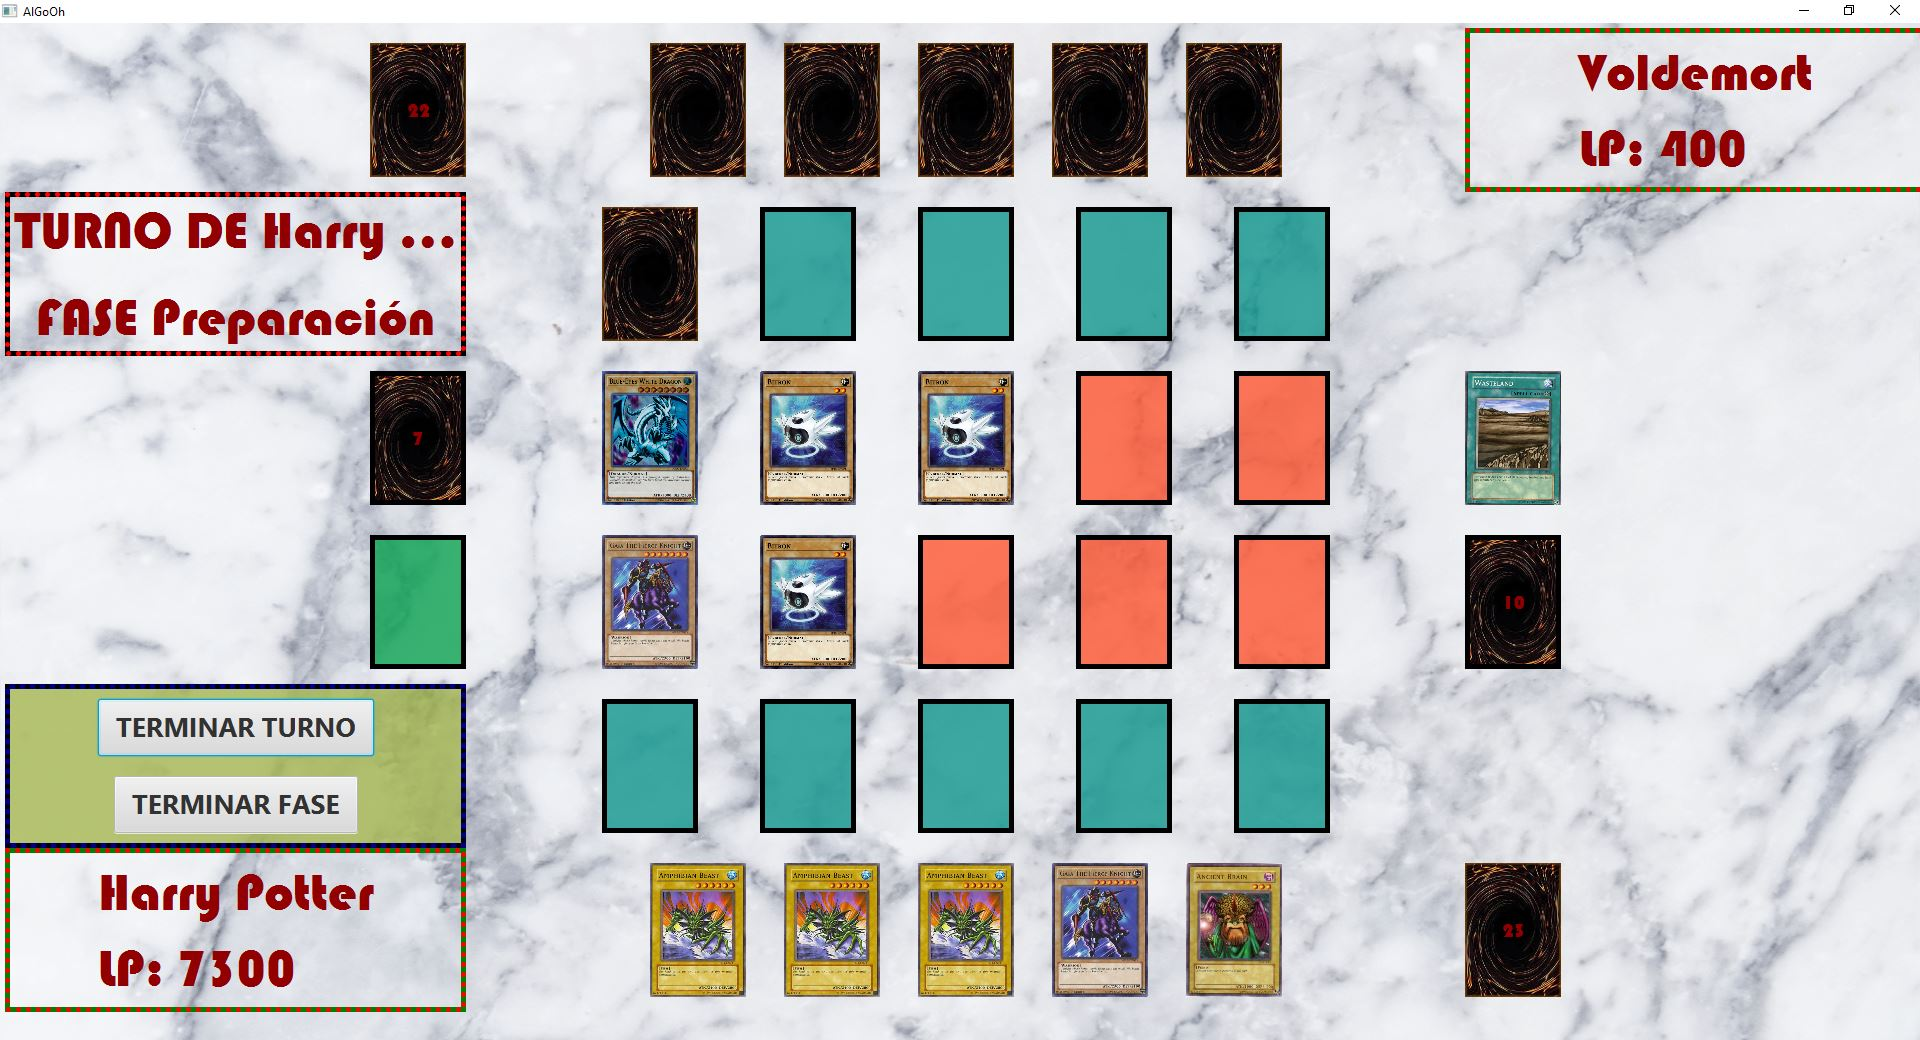
\includegraphics[scale=0.3]{includes/vista_tablero_principal}
		\caption{Vista de tablero principal, donde se puede ver al jugador Harry Potter dándole una lección a Voldermort.}
		\label{vista_tablero_principal}
	\end{figure}
	
	Se hizo uso de la clase \texttt{Tooltip} para mostrar información al usuario de las cartas, como se puede ver en la figura \ref{vista_tooltip_carta}.
	
	Por otro lado, para los ataques de cartas monstruo, se utilizó un menú como el que se muestra en la figura \ref{vista_ataque} para que el jugador seleccione la carta a atacar.
	\begin{figure}[H]
		\centering
		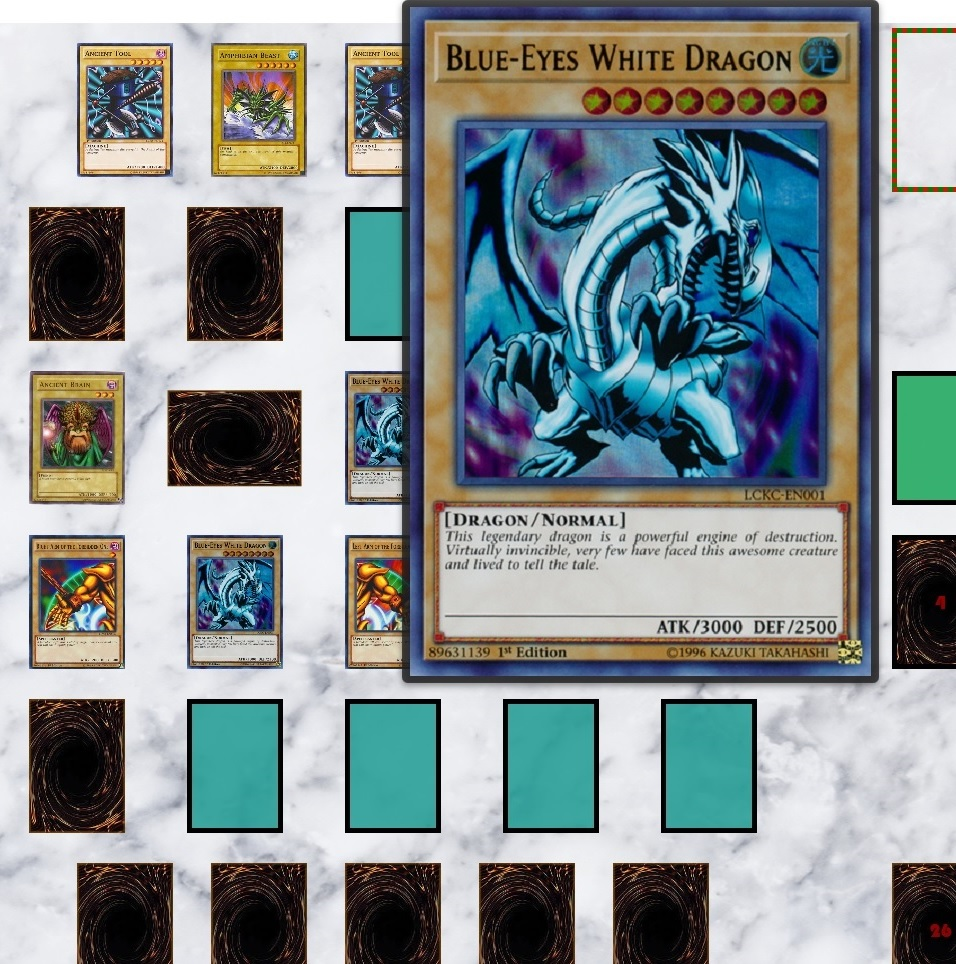
\includegraphics[scale=0.3]{includes/vista_tooltip_carta}
		\caption{Vista de tooltip con información de carta monstruo.}
		\label{vista_tooltip_carta}
	\end{figure}
	
	\begin{figure}[H]
		\centering
		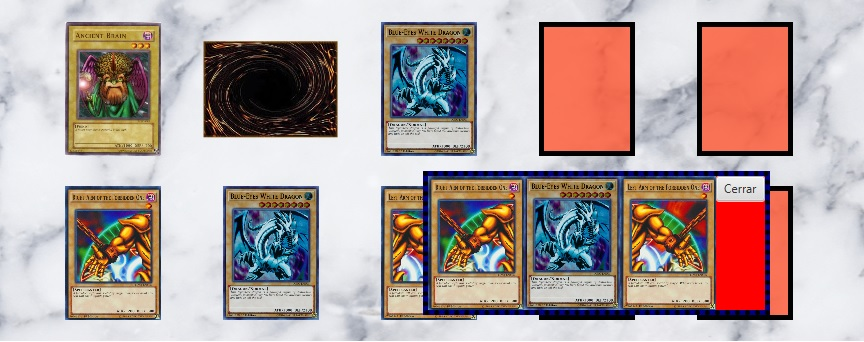
\includegraphics[scale=0.5]{includes/vista_ataque}
		\caption{Menú de ataque.}
		\label{vista_ataque}
	\end{figure}
	
	Para realizar los cambios de turno y fase, se utiliza la clase \texttt{EstadosJuegoBotones} que define los dos botones que puede utilizar el jugador para realizar dichos cambios.
	
	Además, para mostrarle al jugador la información de la fase y turno actual, y de los puntos de vida de cada uno de ellos, se crearon las clases \texttt{TurnoActualVista} y \texttt{VidaVista}.
	
	Por último, para notificar al jugador que no se pueden realizar ciertas acciones, se creó la clase \texttt{ErroresVista} que se encarga de mostrar diferentes advertencias. Por ejemplo, como se puede ver en la figura \ref{vista_errores_jugador}, el jugador \quotes{Voldemort} intentó atacar al jugador \quotes{Harry Potter} en el primer turno, produciéndose la advertencia correspondiente.
	
	\begin{figure}[H]
		\centering
		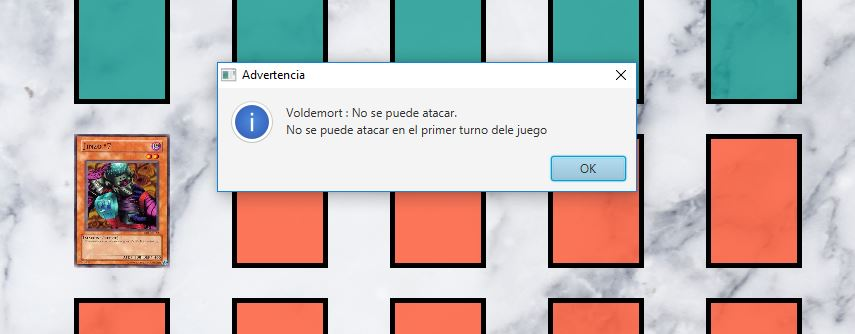
\includegraphics[scale=0.7]{includes/vista_errores_jugador}
		\caption{Voldemort intentando atacar a Harry Potter en el primer turno.}
		\label{vista_errores_jugador}
	\end{figure}
	
	\subsection{Notificación de eventos mediante patrón Observer}
	
	Se decidió utilizar el patrón observer para notificar todos los eventos que ocurren en la aplicación, ya sea para actualizar la escena actual en la vista, como para notificar eventos de fin de juego, o también para saber si entraron cartas a las diferentes regiones para implementar los efectos que existen en el juego.
	
	Particularmente, la clase \texttt{Modelo} implementa diferentes observadores para escuchar eventos de interés, y las clases que observa son:
	\begin{itemize}
		\item \texttt{Carta}, y le notifica si hubo cambios de orientación en la carta.
		\item \texttt{Mano}, y esta le notifica si se agregó o quitó una carta de la mano de cualquiera de los jugadores.
		\item \texttt{Mazo}, y le notifica si se tomó una carta de alguno de los dos mazos.
		\item \texttt{Region}, y le notifica si ingresó o egresó una carta de alguna de las regiones.
		\item \texttt{Jugador}, y le notifica si se modificaron los puntos de vida del mismo, por ejemplo, durante un ataque.
	\end{itemize}
	
	Con esta información, la clase \texttt{Modelo} le notifica a la Vista para que la misma actualice su estado y le muestre al jugador el evento ocurrido.
	
	Por otro lado, se tiene la clase \texttt{RegionCampo} que observa a las regiones monstruo del jugador y del oponente para activar o desactivar el efecto de la carta campo activa actualmente (si es que la hay) cuando ingresa o egresa una carta monstruo de dichas regiones.
	
	\subsubsection{Observador de fin de juego}
	
	Para saber si se cumple alguna de las condiciones de fin de juego, se definen las interfaces \texttt{FinDeJuegoObservable} y \texttt{ObservadorDeFinJuego} para notificar al Controlador de que se llegó al fin de juego, para que este realice las tareas necesarias de terminación. Entre otras, mostrar la pantalla de salida al usuario.
	
	Las clases que son responsables de notificar un fin de juego son \texttt{Mazo}, \texttt{Mano}, y \texttt{Jugador}, ya que pueden darse las diferentes causas de fin de juego en ellas. Por ejemplo, si el mazo de algún jugador se queda sin cartas, va a notificar tal evento para finalizar la partida.
	
	Las diferentes causas de fin de juego se encuentran dentro del paquete \texttt{finDeJuego}, y todas derivan de la clase abstracta \texttt{CausaFinJuego}. En la misma se define el método \texttt{getNombreCausa()} que es utilizado por la vista para mostrarle al jugador cuál fue la causa de fin de partida.
	
	
	
	\subsection{Utilización de patrón Singleton}
	
	Hay varias clases en las que se requiere una sola instancia de las mismas durante la aplicación. Por ello, se decidió utilizar el patrón Singleton para evitar que el cliente de las clases cree más de una de ellas.
	
	Hay varias de ellas, pero las más importantes son \texttt{Controlador}, \texttt{Modelo}, las diferentes fases del juego, \texttt{MaquinaTurnos}, \texttt{VerificadorCondicionesJuego}, y las diferentes clases \quotes{nulas}: \texttt{CartaTrampaNula}, \texttt{CartaMonstruoNula}, \texttt{CartaNula}, \texttt{FaseNula}, \texttt{CausaFinJuegoNula}, etc...
	
	\clearpage
	\section{Diagramas de clases}
	
	A continuación se muestran los diagramas de clase estáticos. Debido a la extensión del trabajo, se decidió mostrar solamente las clases y métodos más importantes, por lo que se refiere al lector al código fuente para estudiar los detalles de implementación.
	
	\subsection{Carta}
	
	En la figura \ref{class_Carta} se muestra como está organizada la clase Carta. Como ya se mencionó anteriormente, Carta es una clase abstracta, la cual es \quotes{padre} de todos los tipos de cartas en el juego (hablaremos de cada una de ellas más adelante). Todas las cartas son creadas en la Fábrica de Cartas, figura \ref{class_FabricaCartas}.
	
	\begin{figure}[H]
		\centering
		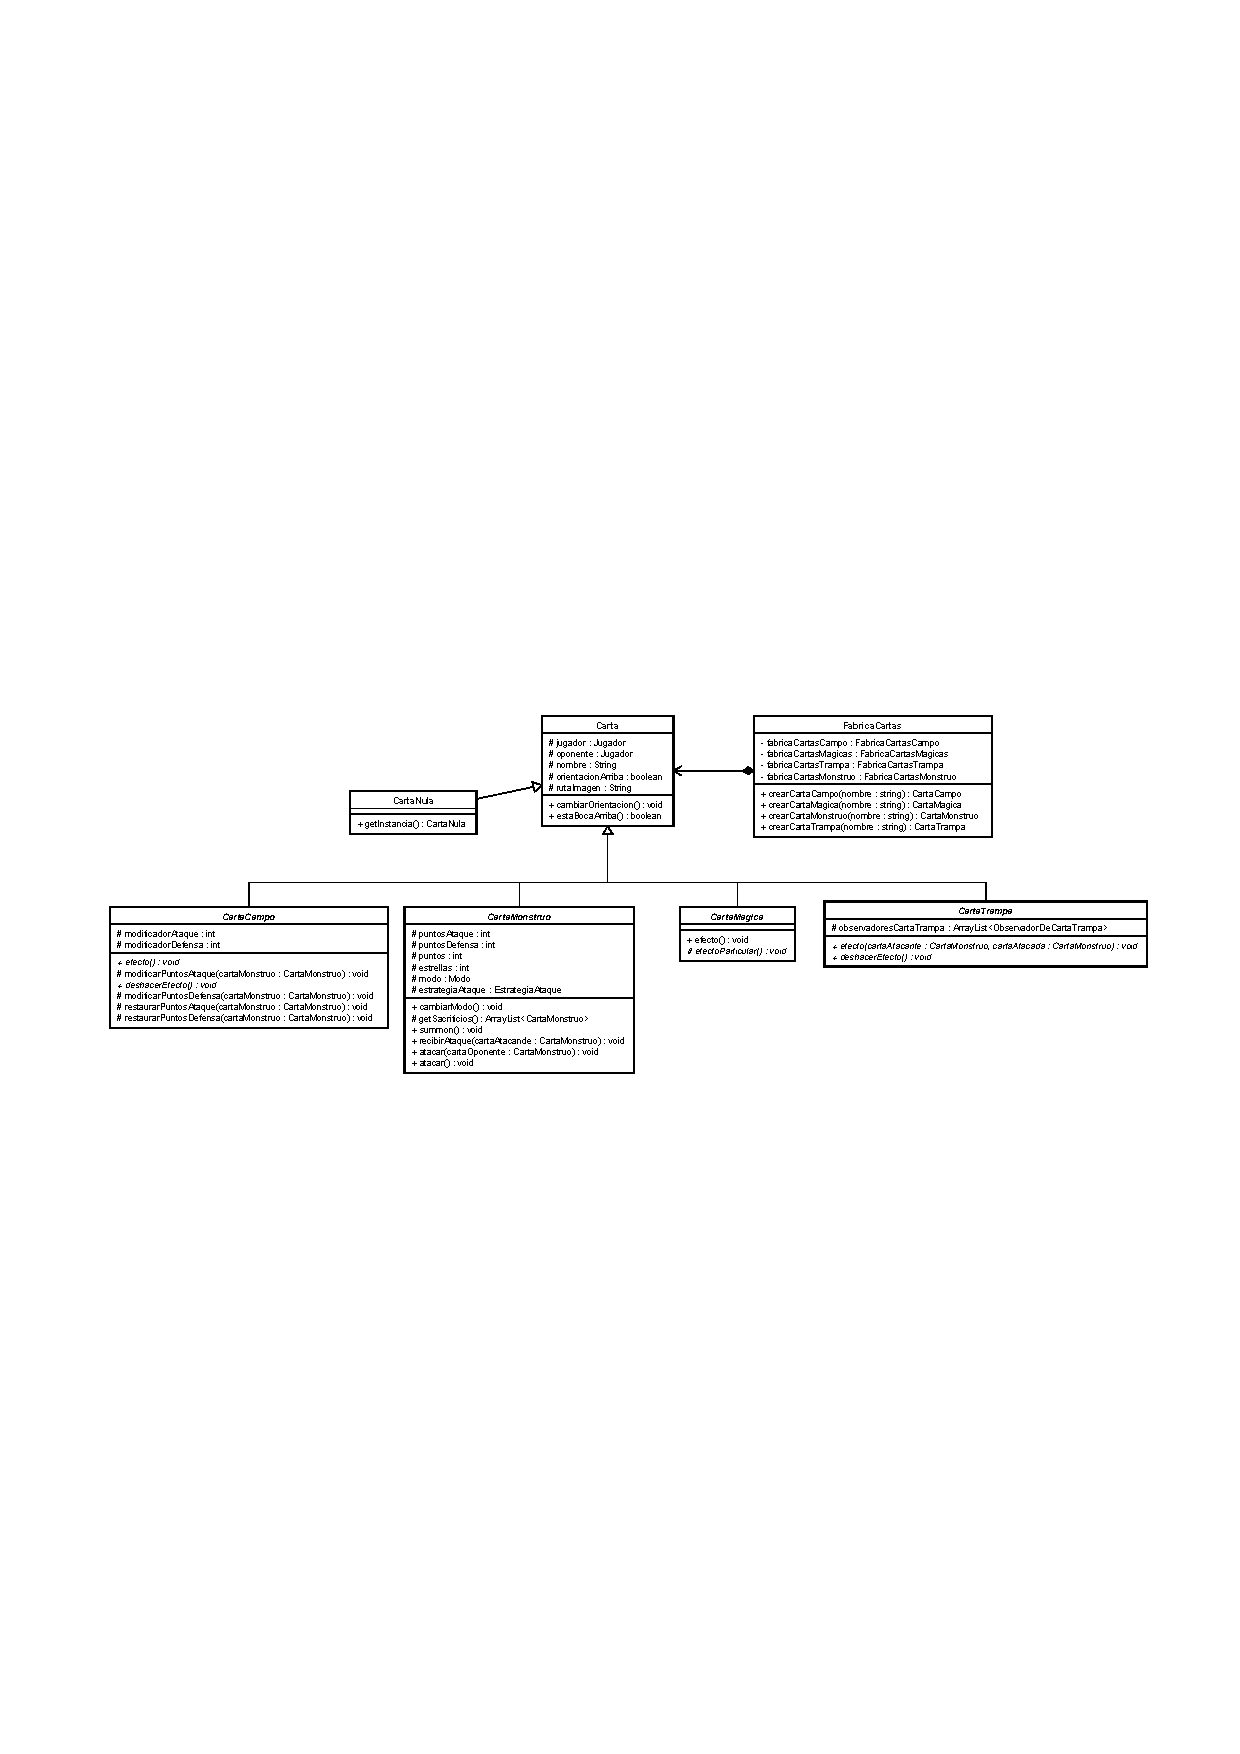
\includegraphics[scale=0.8]{includes/class_Carta}
		\caption{Diagrama de la clase Carta}
		\label{class_Carta}
	\end{figure}
	
	\subsection{Carta Monstruo}
	
	En la figura \ref{class_CartaMonstruo} notamos que este tipo de cartas tienen un \texttt{Modo} y una \texttt{EstrategiaAtaque}. El modo nos dice, como muestra la figura, si la carta esta en ataque o defensa. De esto va a depender ya sea con que puntos (Puntos de ataque o puntos de defensa) se realiza el cálculo para determinar que carta \quotes{gana} en caso de un ataque y las opciones que tiene la carta cuando ya fue jugada. Por ejemplo, una carta en modo defensa no puede atacar.
	
	En cuanto a la \texttt{EstrategiaAtaque}, esta es la entidad que se encarga de \quotes{ejecutar} el ataque. Fue creada ya que en el juego, pueden ocurrir situaciones en las cuales un ataque no es el común, por ejemplo, como se muestra en la figura, el caso en el cual una carta \texttt{MagicCylinder}
	
	
	\begin{figure}[H]
		\centering
		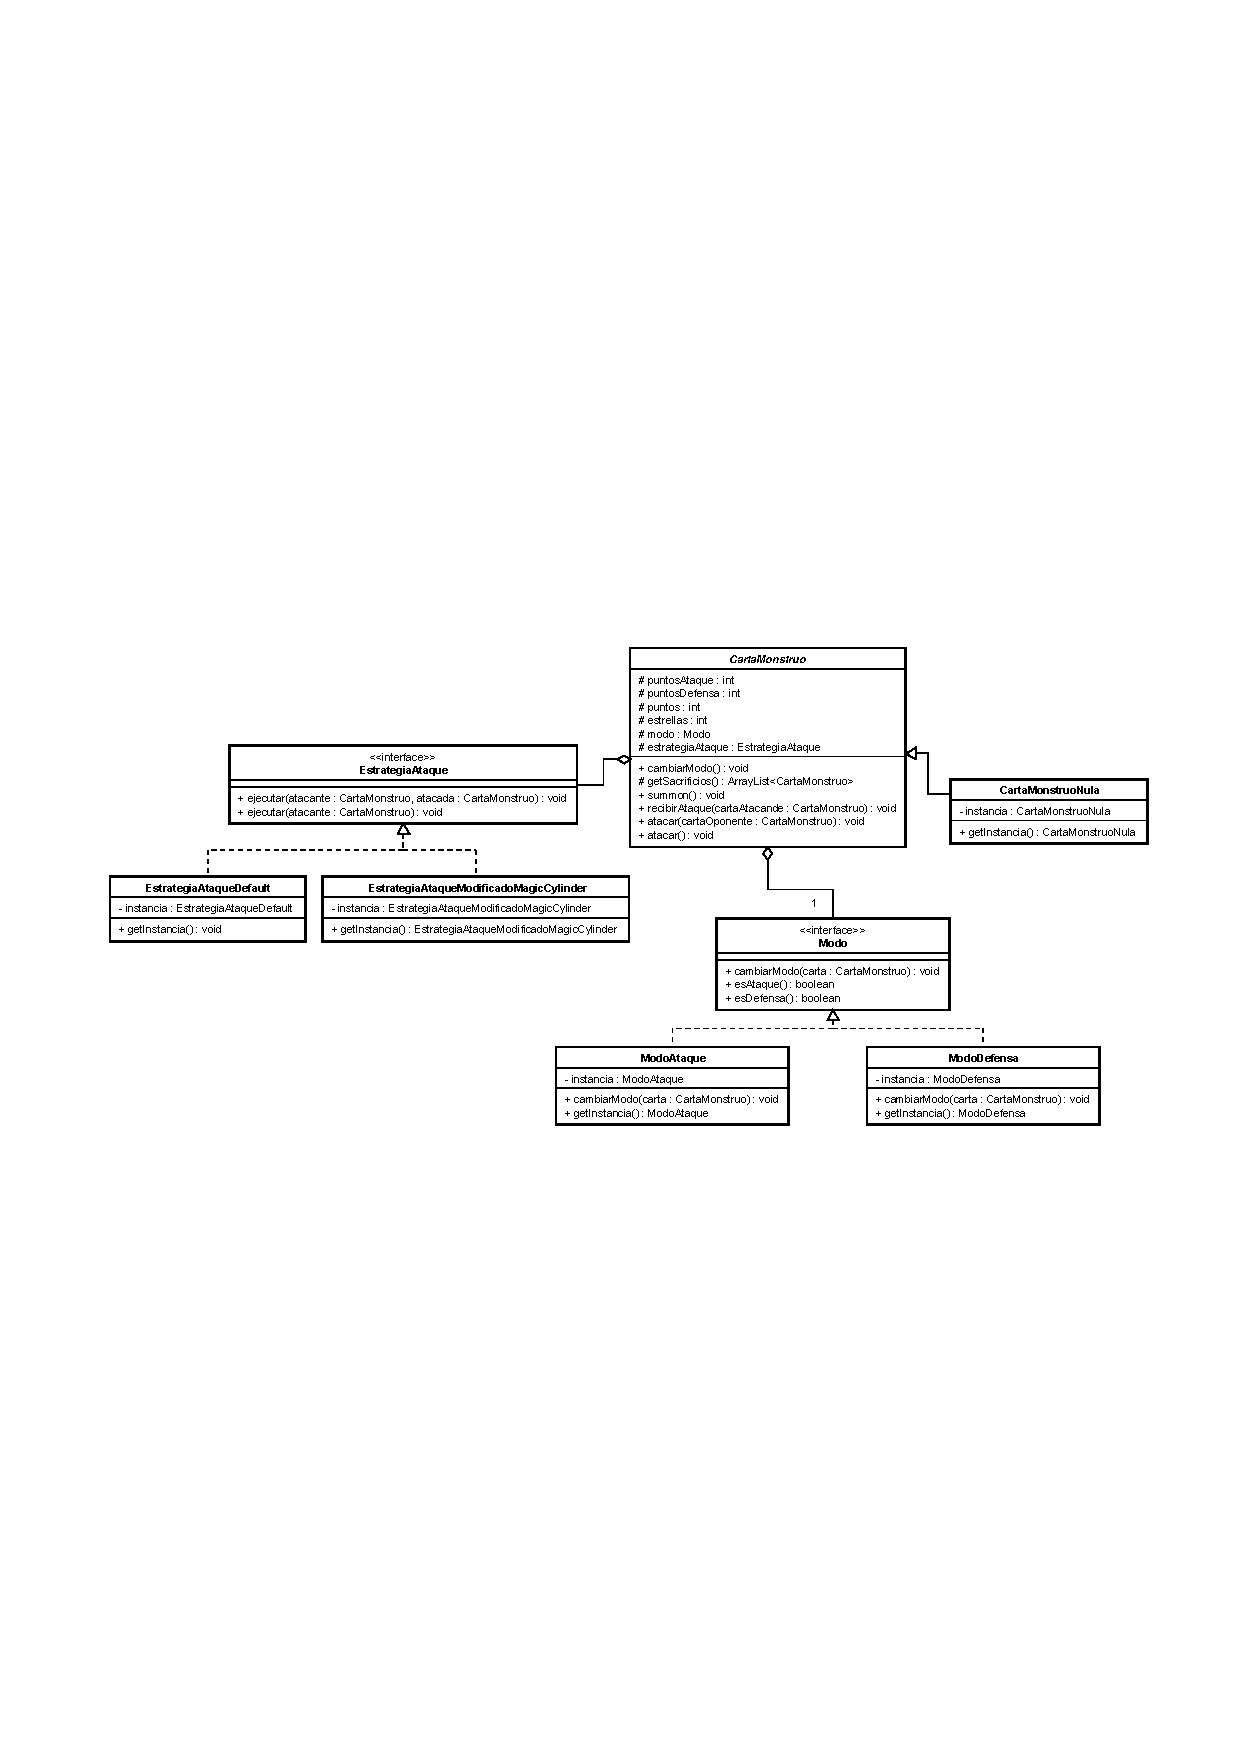
\includegraphics[scale=0.8]{includes/class_CartaMonstruo}
		\caption{Carta Monstruo.}
		\label{class_CartaMonstruo}
	\end{figure}
	
	
	\subsection{Carta Trampa}
	
	Refiriéndose a la figura \ref{class_Carta_Trampa}, la característica principal que vemos es que este tipo de cartas tienen un efecto y, además, pueden influir en como se ejecuta un ataque de una \texttt{CartaMonstruo} (como ejemplificamos anteriormente con la carta \texttt{MagicCylinder}). El efecto de la carta es diferente para cada una de las \texttt{CartaTrampa}.
	
	\begin{figure}[H]
		\centering
		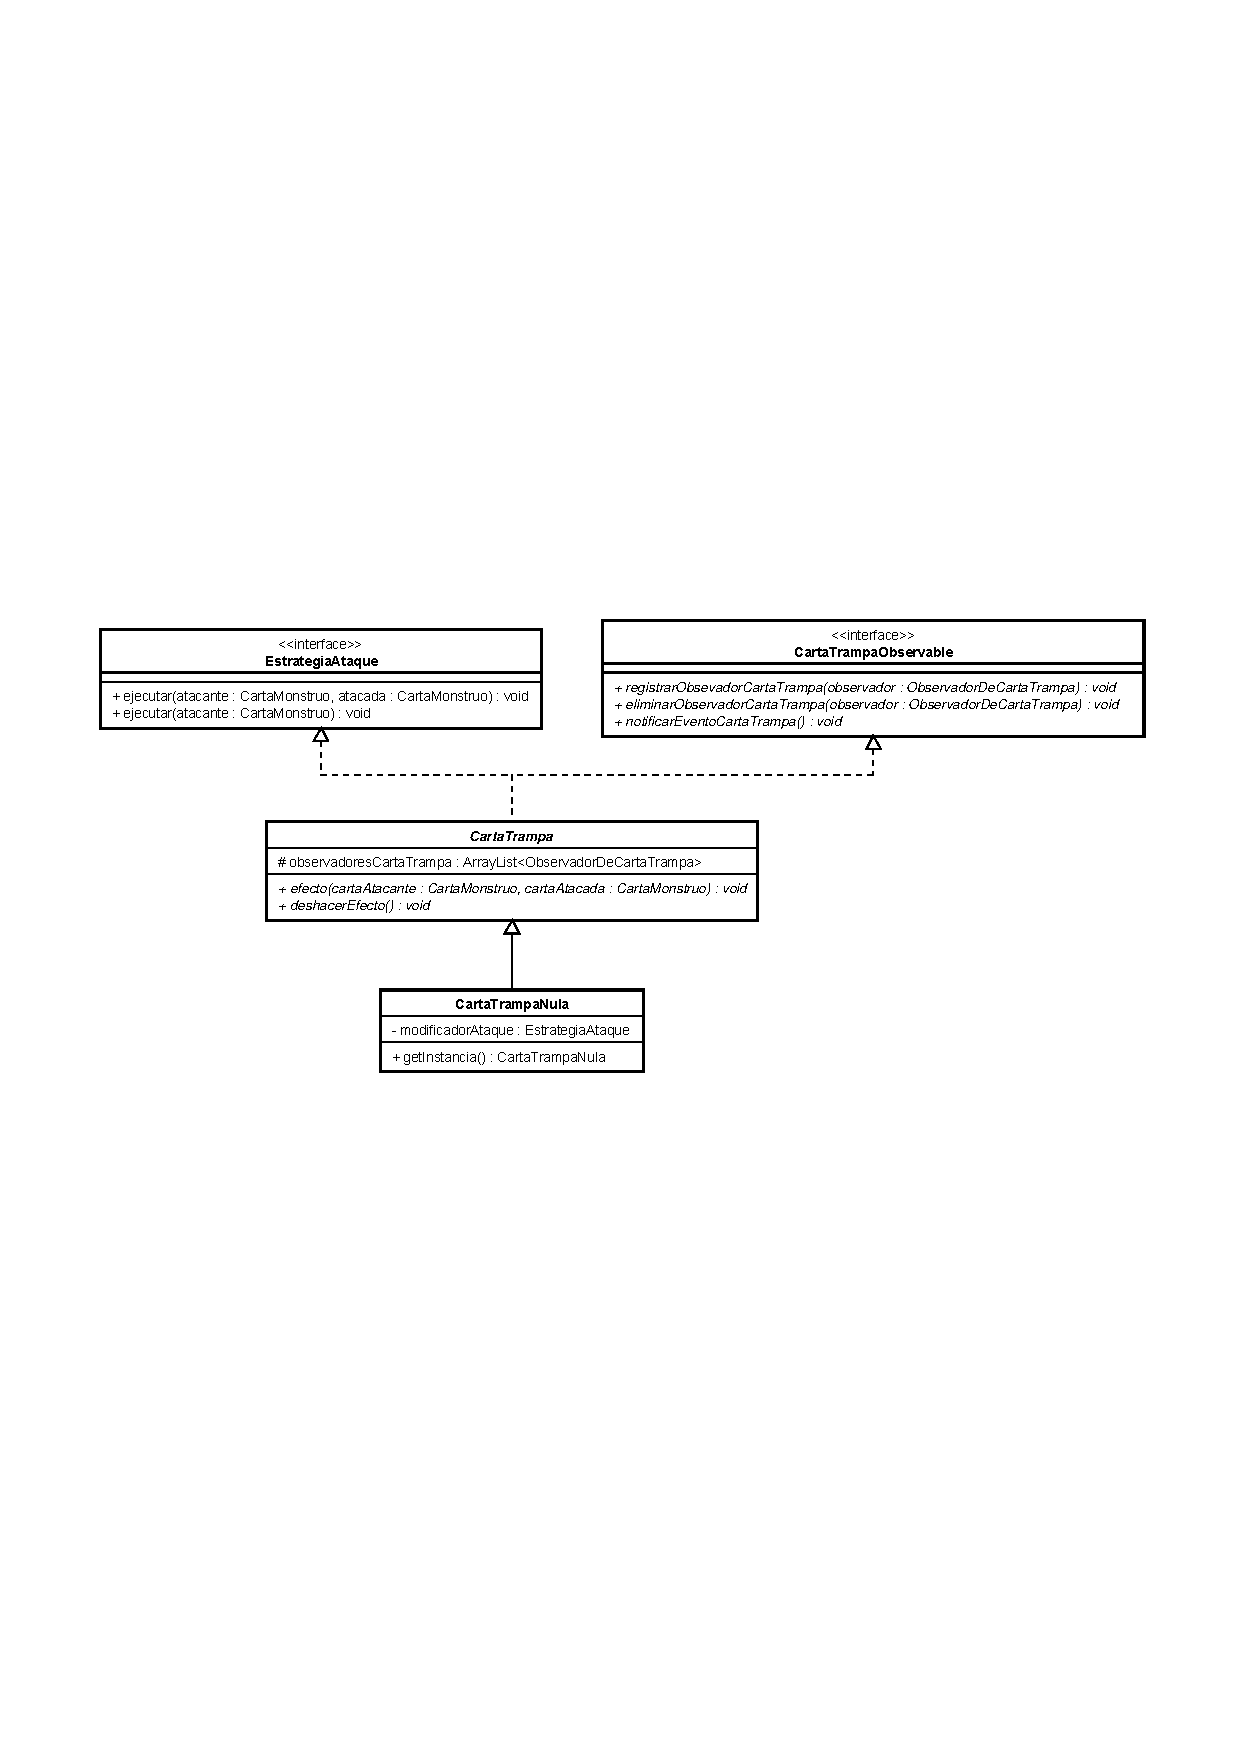
\includegraphics[scale=0.8]{includes/class_CartaTrampa}
		\caption{Carta Trampa}
		\label{class_Carta_Trampa}
	\end{figure}
	
	\subsection{Causa Fin de Juego}
	
	Figura \ref{class_CausaFinJuego}: Causa fin de juego. El \quotes{juego} puede terminar por diversas razones, por lo que se crearon clases para cada una de las posibilidades de fin de juego, las cuales, a medida que corre el programa, se encargan de verificar, interactuando con otros elementos del modelo, que se hayan o no cumplido las condiciones para que termine el juego.
	
	\begin{figure}[H]
		\centering
		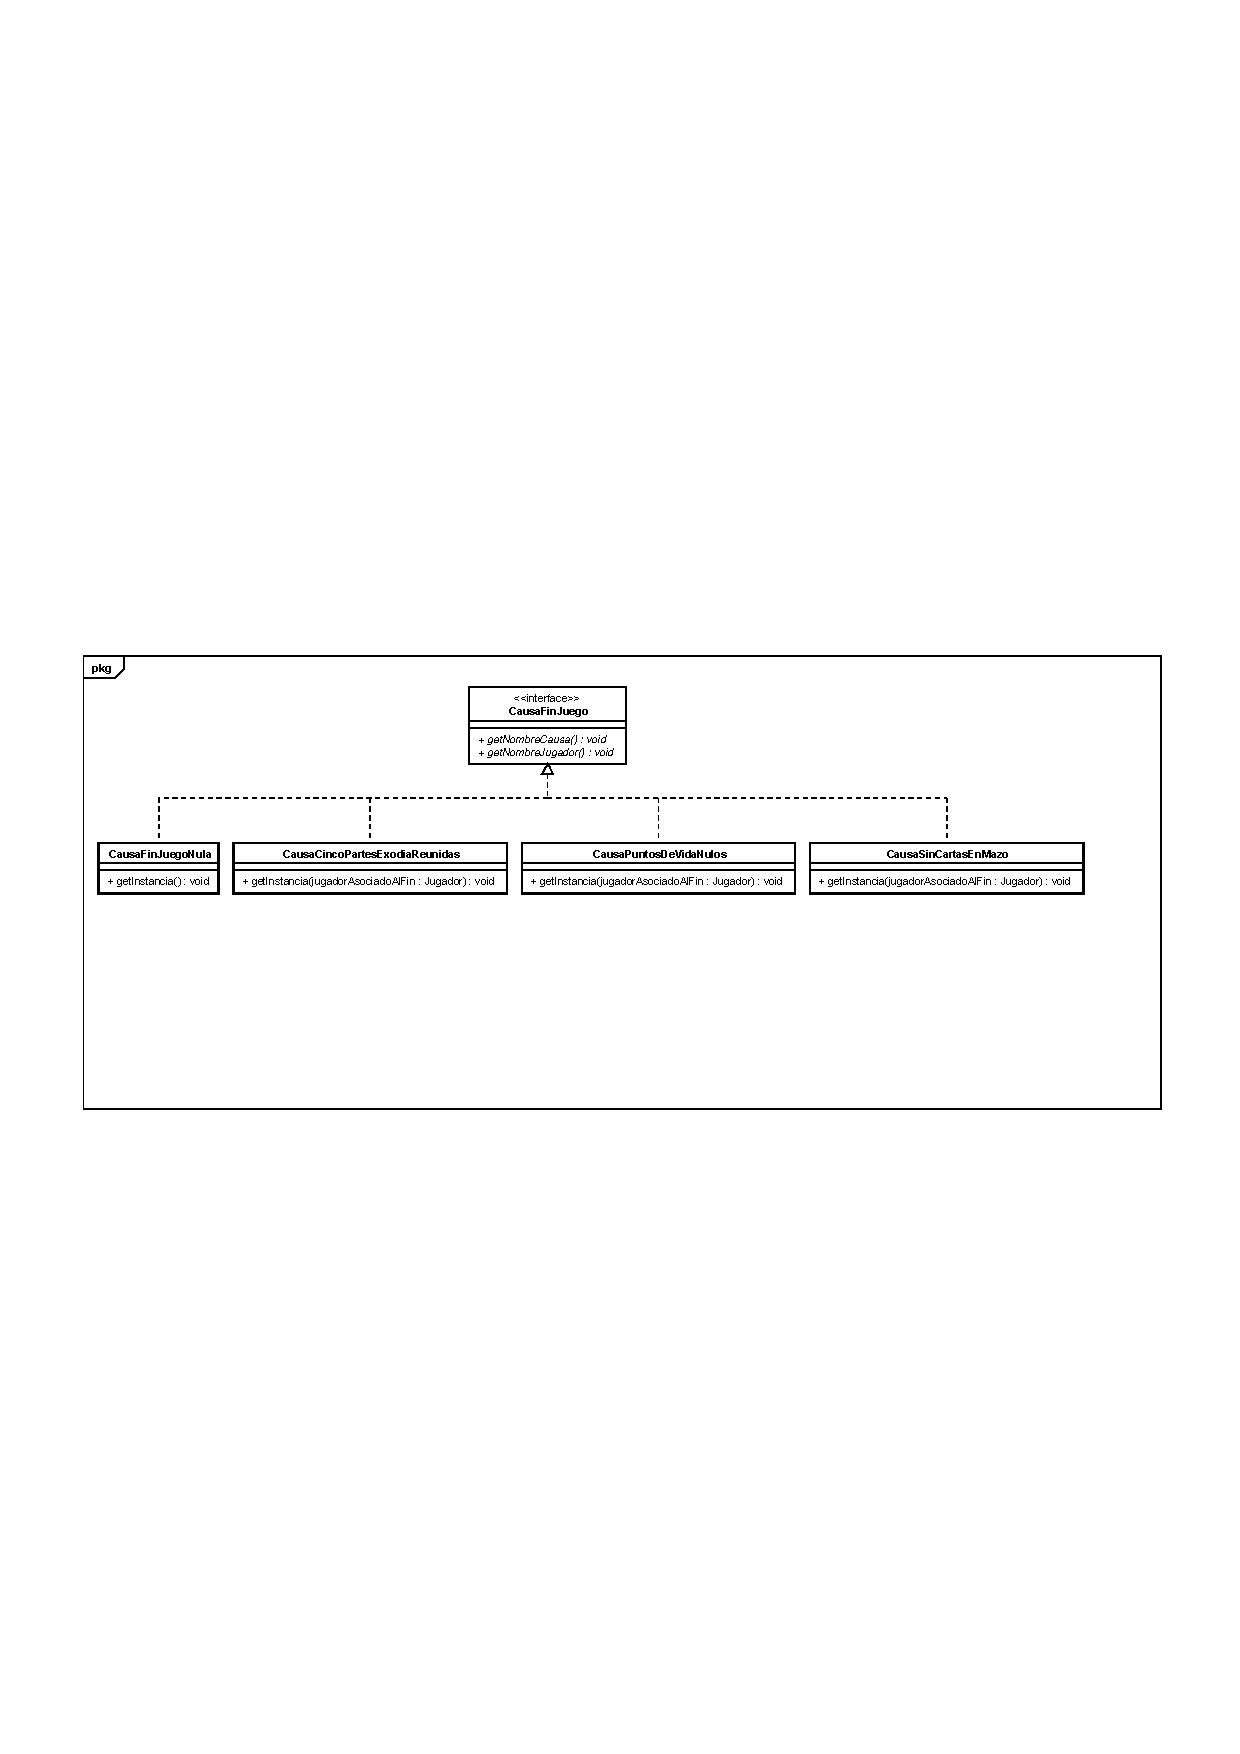
\includegraphics[scale=0.8]{includes/class_CausaFinJuego}
		\caption{Causa Fin de Juego.}
		\label{class_CausaFinJuego}
	\end{figure}
	
	\subsection{Controlador}
	
	Aquí (Figura \ref{class_Controlador}) vemos como aparece el patrón MVC mirándolo desde el \texttt{Controlador}. Este tiene relaciones con el \texttt{Modelo} al igual que con la \texttt{Vista} y tiene dentro de el a
	\texttt{VerificadorCondicionesJuego}, clase que se encarga de realizar las verificaciones necesarias para habilitar o no una acción del \texttt{Jugador}.
	
	\begin{figure}[H]
		\centering
		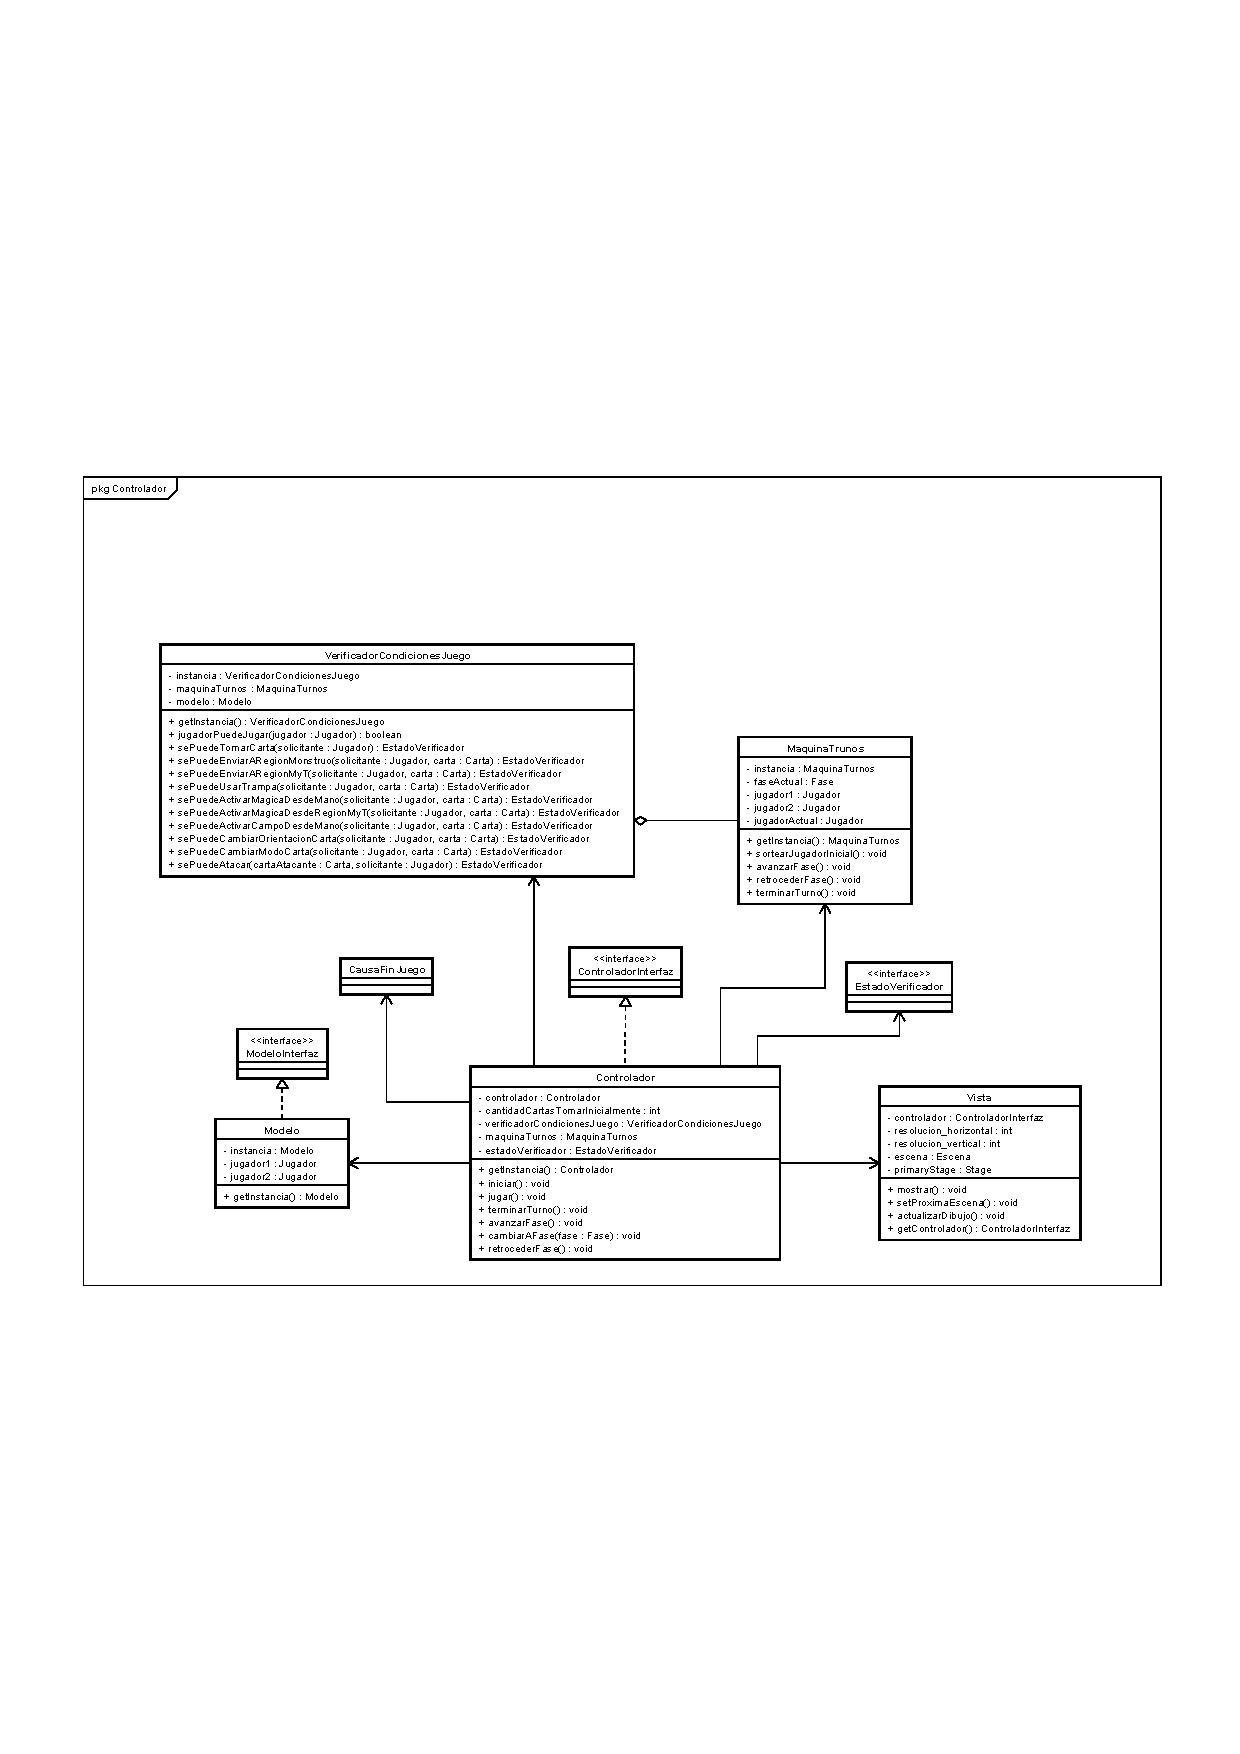
\includegraphics[scale=0.8]{includes/class_Controlador}
		\caption{Controlador.}
		\label{class_Controlador}
	\end{figure}
	
	\subsection{Fábrica de Cartas}
	
	En el diagrama (\ref{class_FabricaCartas}) podemos ver a la \texttt{FabricaDeCartas} y sus 4 \quotes{SubFabricas}. Como se ve en la figura, tenemos una Fabrica para cada tipo de carta. Cada una de estas fabricas es creada con todas las cartas posibles del tipo especificado dentro de ella, lo que quiere decir que, todas las diferentes \texttt{CartasMonstruo} son creadas dentro de \texttt{FabricaCartasMonstruo}, luego, la \texttt{FabricaDeCartas} le pide a la \texttt{FabricaCartasMonstruo} la carta específica que quiere.
	
	Como se menciono en la nota del diagrama, la cantidad de cartas que tenemos en cada fábrica es limitada. Pero de la forma que fueron hechas, si en algún punto queremos agregar, por ejemplo, una nueva \texttt{CartaMonstruo}, alcanza con crearla con sus respectivos puntos de ataque, defensa y efectos dentro de la \texttt{FabricaCartasMonstruo} para que pueda ser usada en el juego.
	
	\begin{figure}[H]
		\centering
		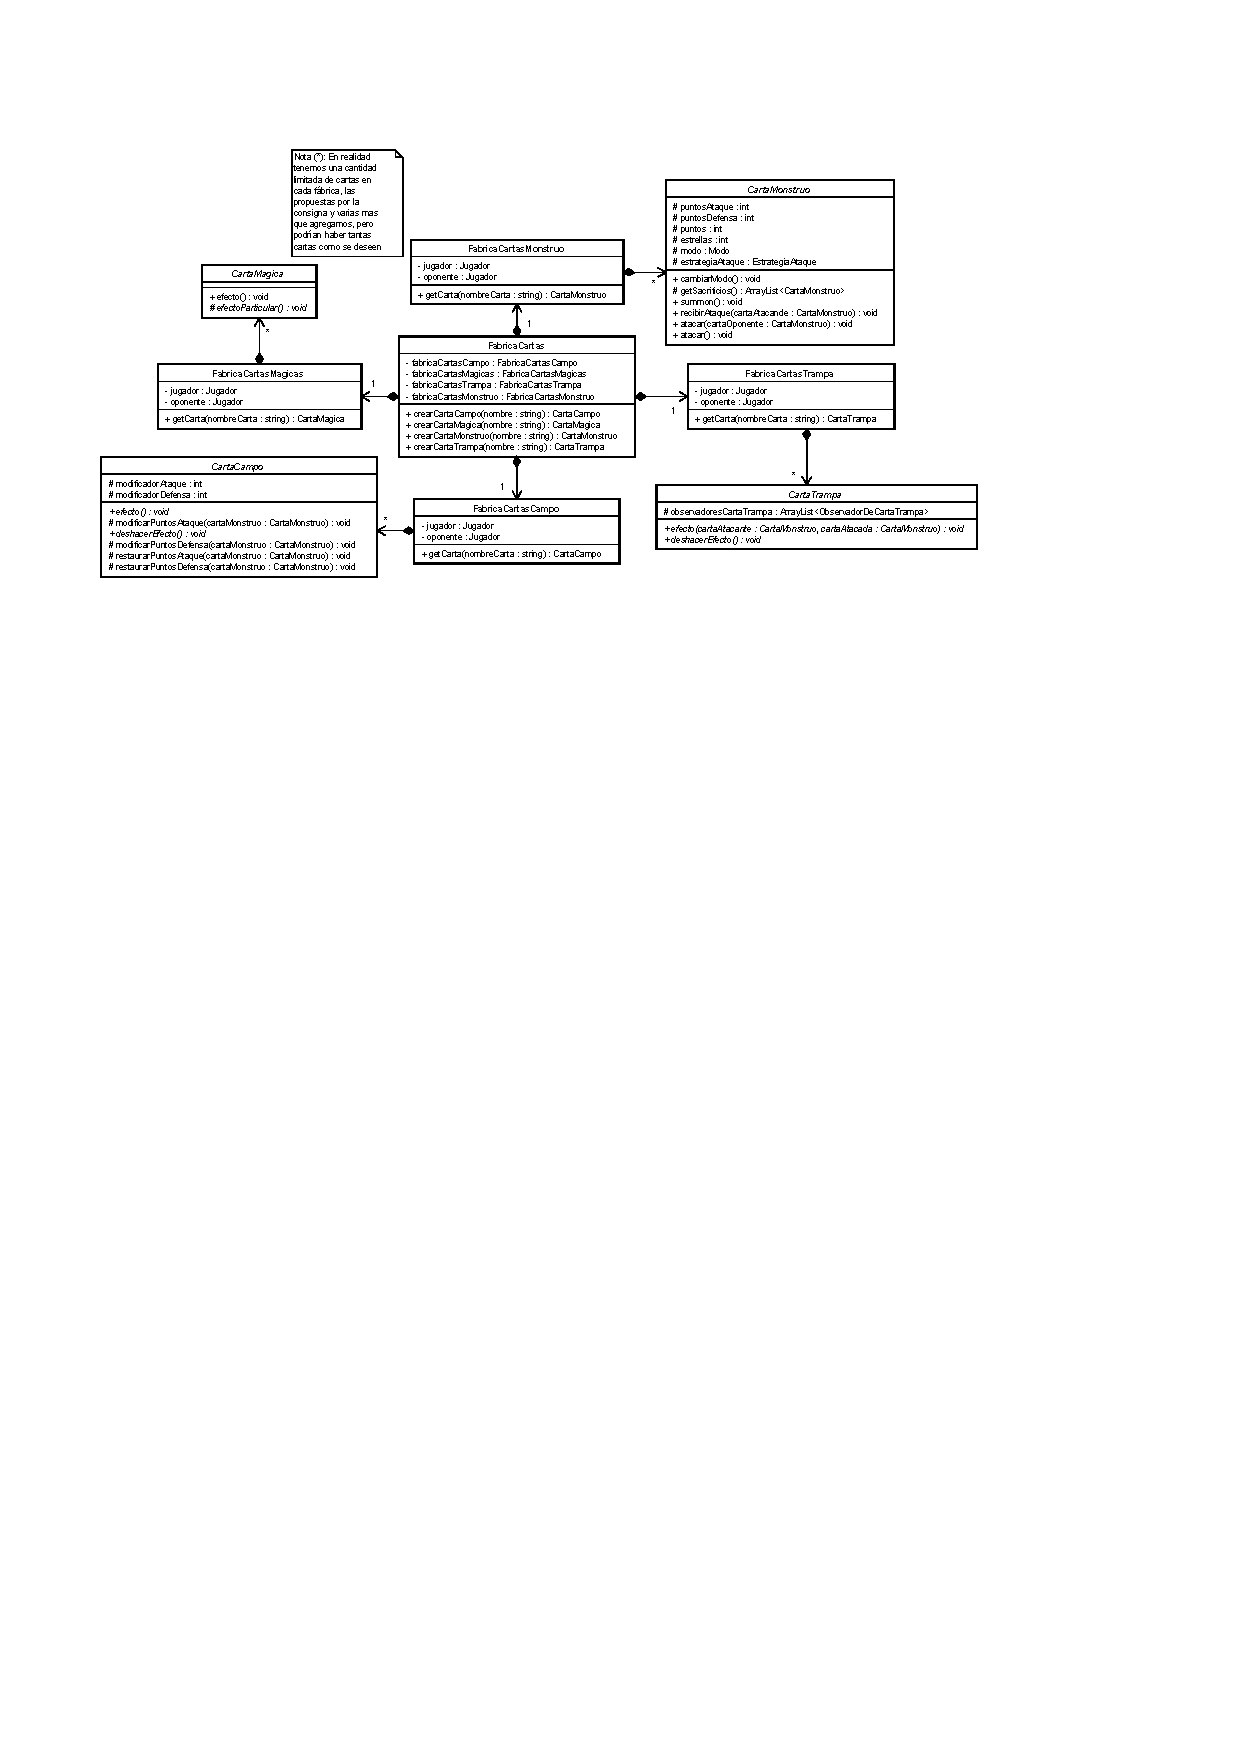
\includegraphics[scale=0.8]{includes/class_FabricaCartas}
		\caption{Fábrica de Cartas.}
		\label{class_FabricaCartas}
	\end{figure}
	
	\subsection{Jugador}
	
	Aquí vemos (Figura \ref{class_Jugador}) como esta compuesto el \texttt{Jugador}. Éste, como se menciono anteriormente, esta compuesto por su oponente (otro \texttt{Jugador}) su \texttt{Mano}, \texttt{Mazo} y 4 \texttt{Regiones} (Figura \ref{class_Regiones}).
	
	\begin{figure}[H]
		\centering
		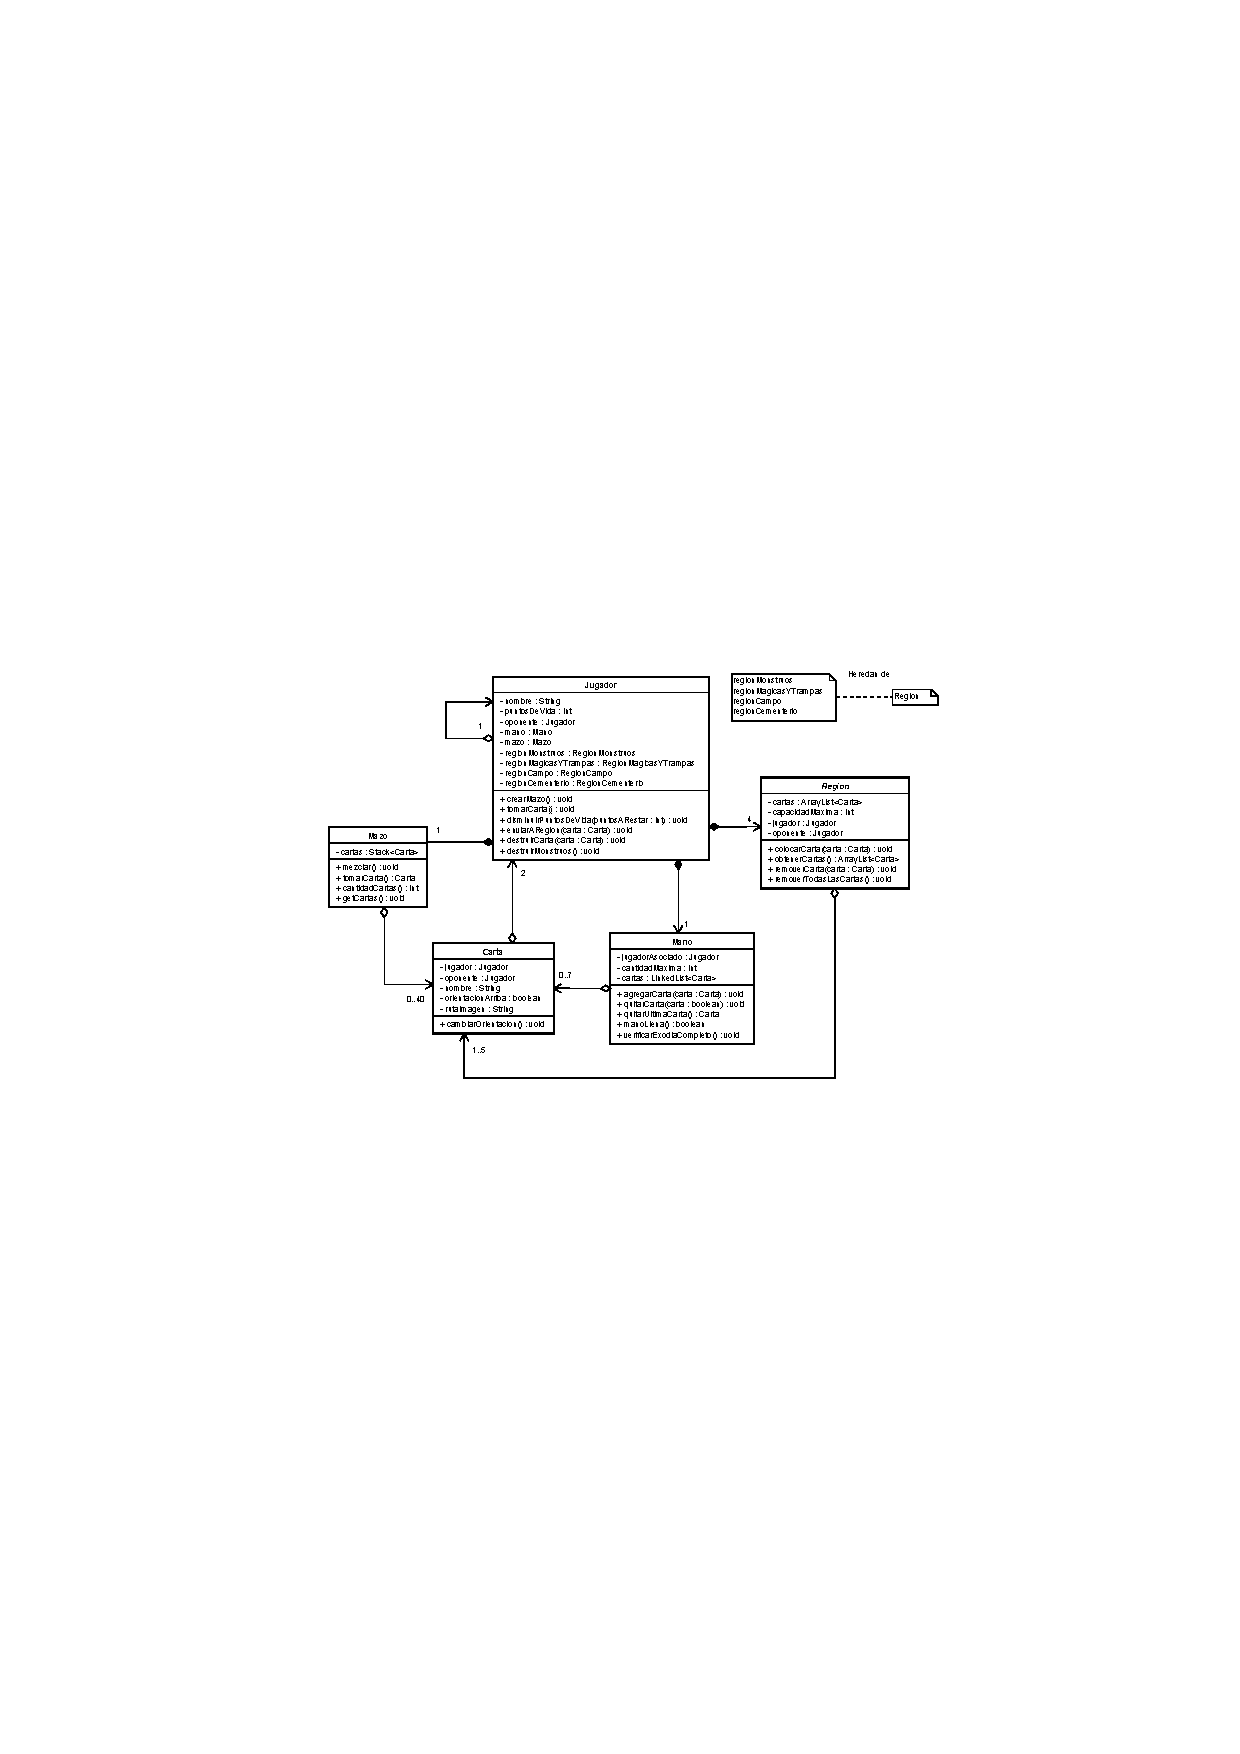
\includegraphics[scale=0.8]{includes/class_Jugador}
		\caption{Jugador.}
		\label{class_Jugador}
	\end{figure}
	
	\subsection{Modelo}
	
	El diagrama a continuación (Figura \ref{class_Modelo}) muestra los métodos mas importantes en la interfaz \texttt{ModeloInterfaz}. Estos métodos son los que la clase \texttt{Controlador} usa para realizar cambios en el \texttt{Modelo} a partir de las acciones que realiza el usuario en la \texttt{Vista}.
	
	\begin{figure}[H]
		\centering
		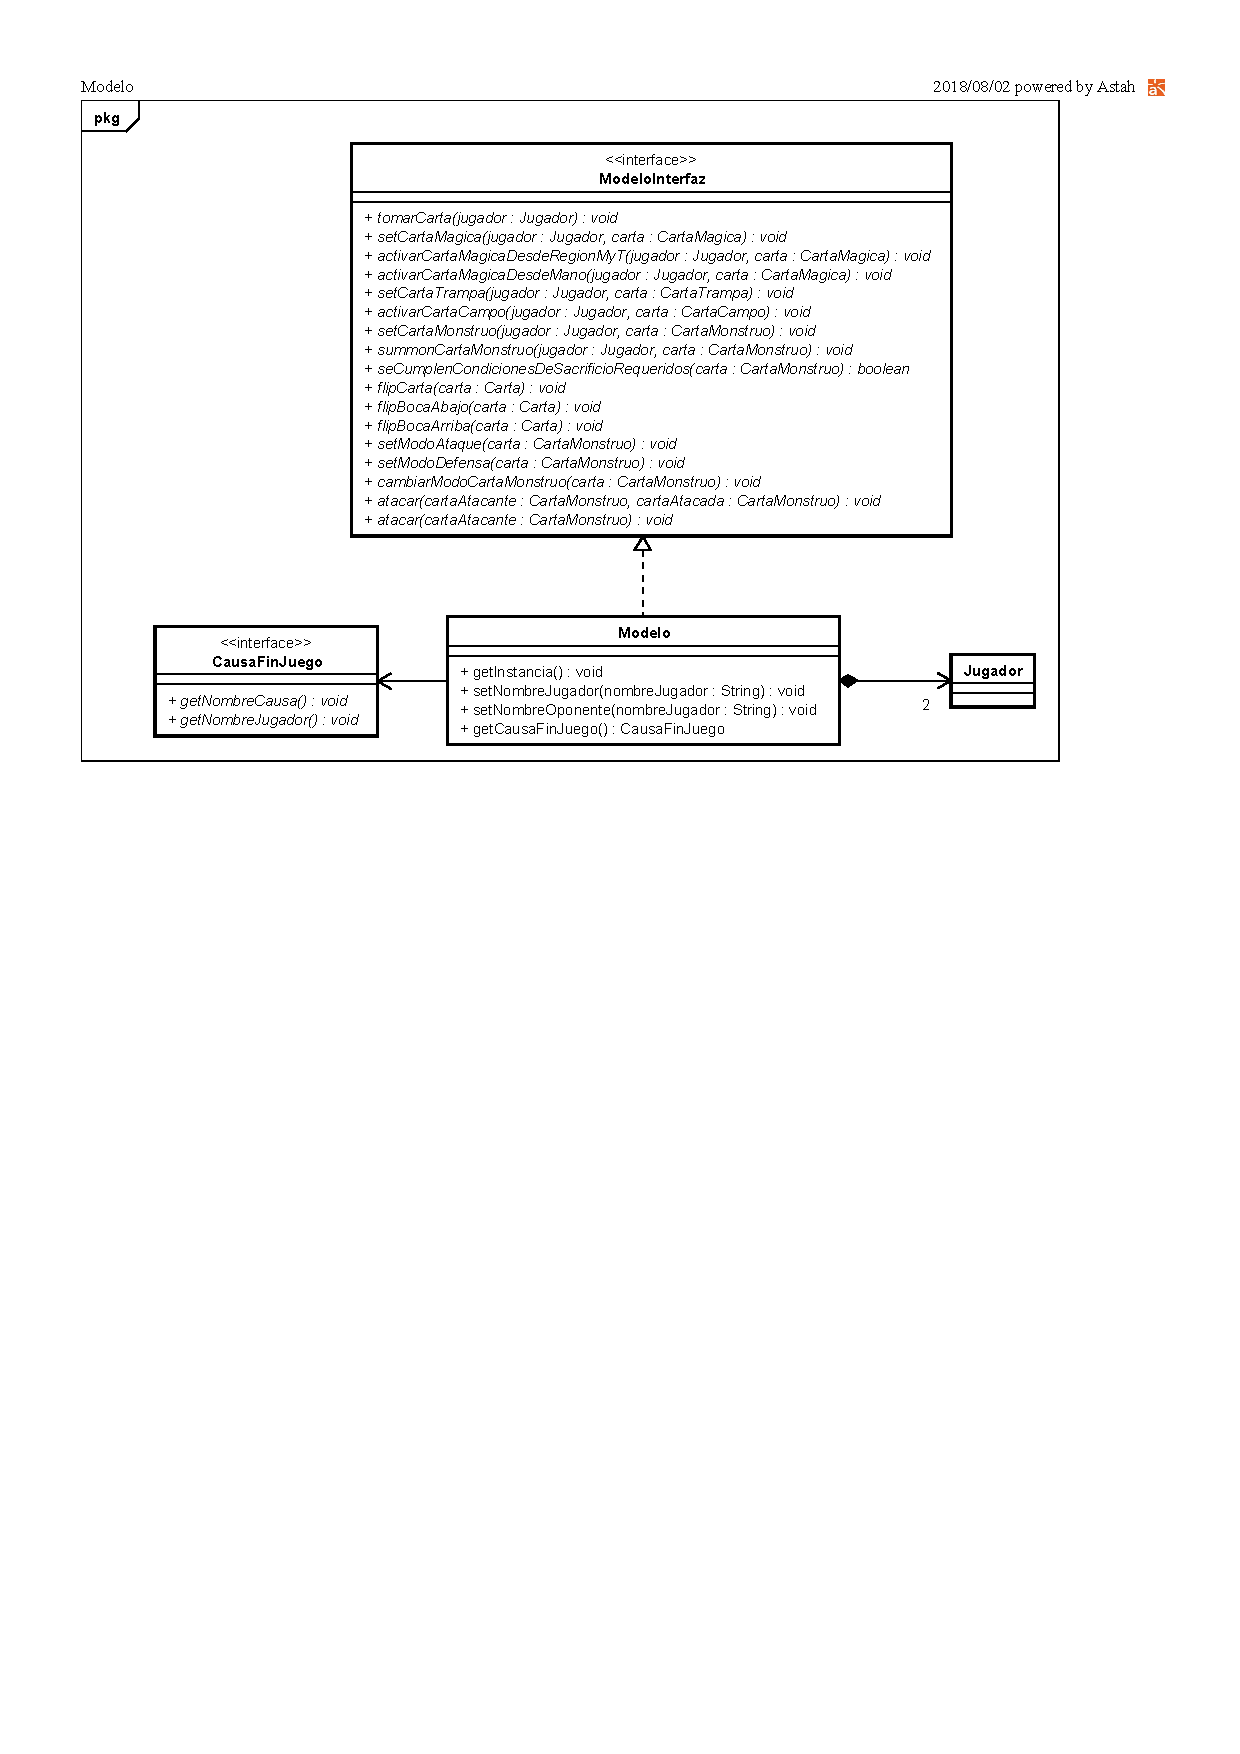
\includegraphics[scale=0.8]{includes/class_Modelo}
		\caption{Modelo}
		\label{class_Modelo}
	\end{figure}
	
	\subsection{Observadores}
	
	En el diagrama (Figura \ref{class_Observadores}) se pueden ver todas las relaciones entre los observadores del juego, para facilitar la comprensión solo se nombraron los métodos más importantes de cada \texttt{Observador}.
	
	\begin{figure}[H]
		\centering
		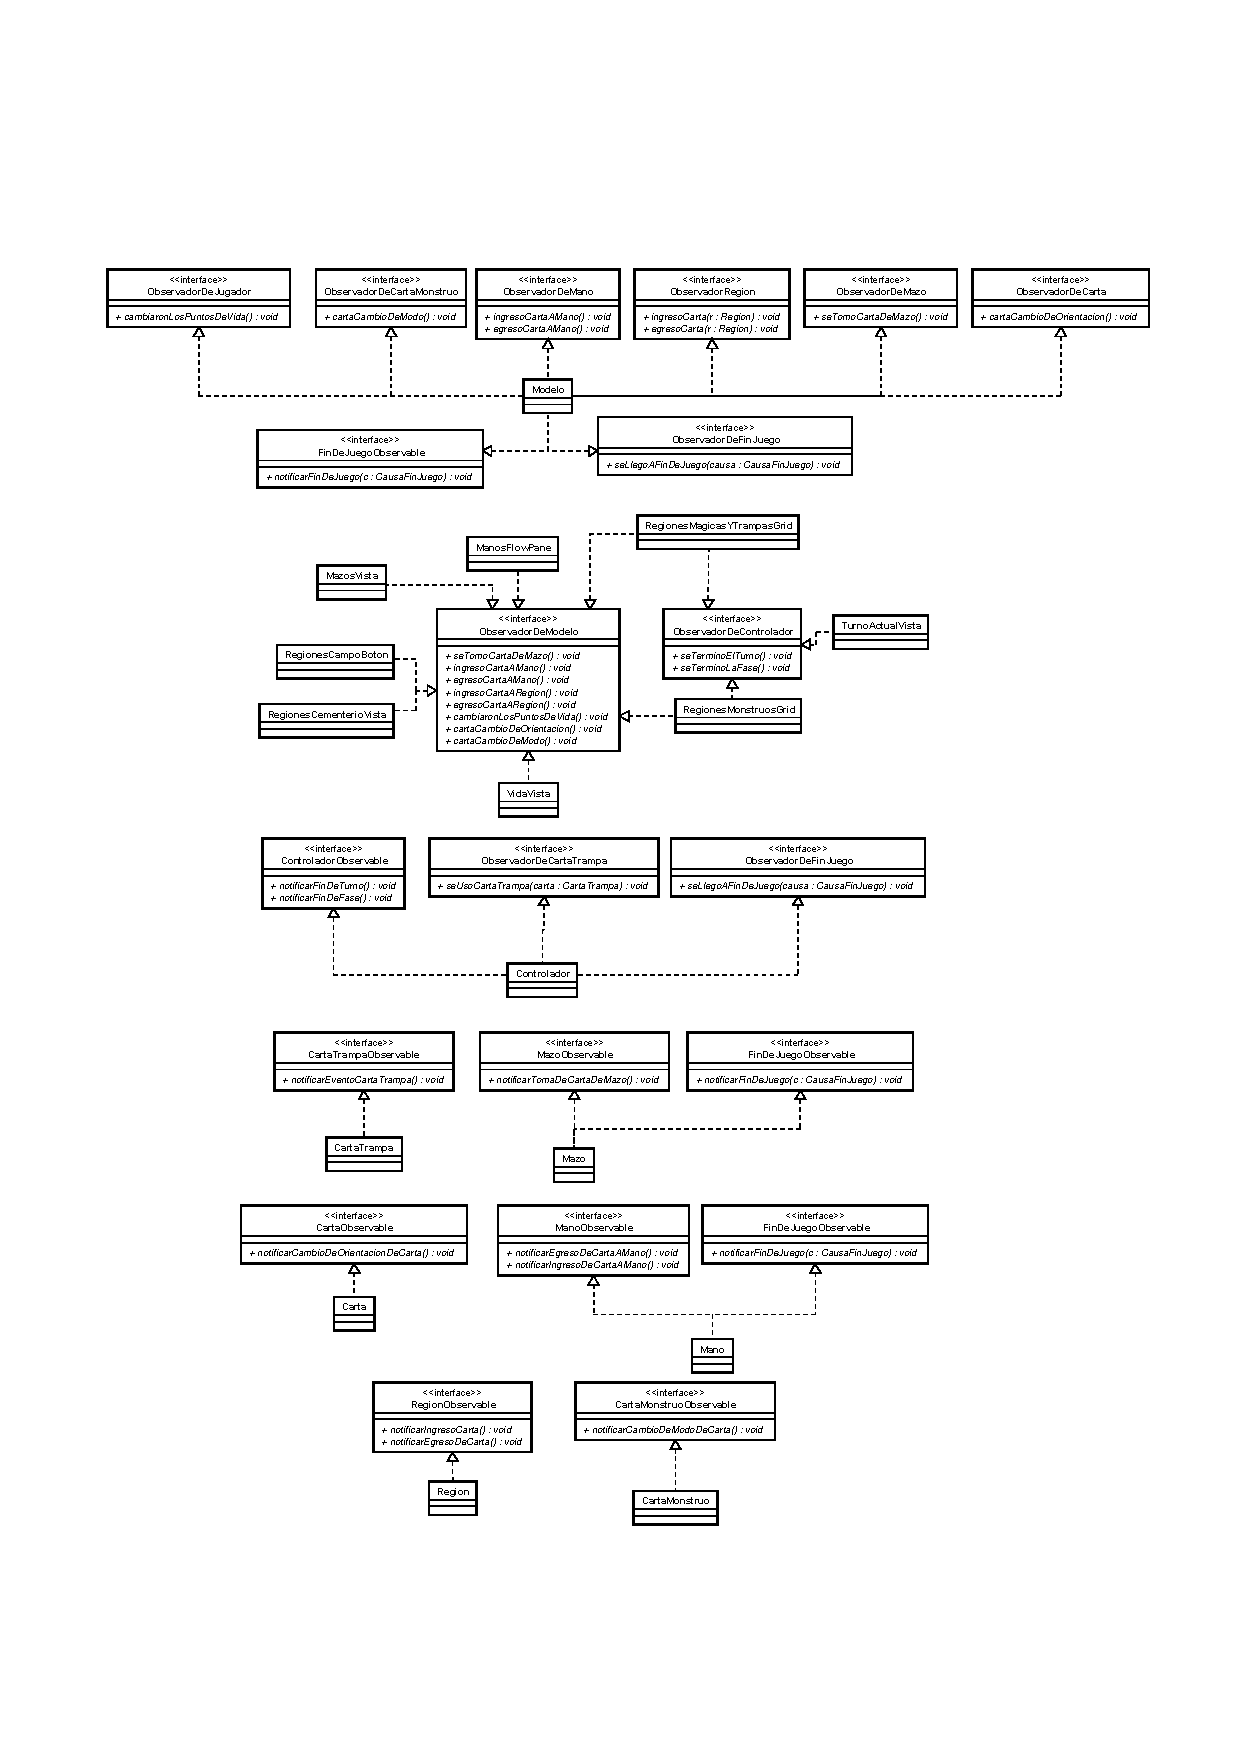
\includegraphics[scale=0.8]{includes/class_Observadores}
		\caption{Observadores.}
		\label{class_Observadores}
	\end{figure}
	
	\subsection{Regiones}
	
	La figura \ref{class_Regiones} muestra la relación de herencia entre los distintos tipos de regiones (\texttt{RegionCampo}, \texttt{RegionMonstruos}, \texttt{RegionCementerio} y \texttt{RegionMagicasYTrampas}) con su clase \quotes{padre} \texttt{Region}, con algunos métodos generales para todas las regiones, pertenecientes a la clase abstracta \texttt{Region} y específicos para cada una de sus diferentes clases \quotes{hijas}.
	
	\begin{figure}[H]
		\centering
		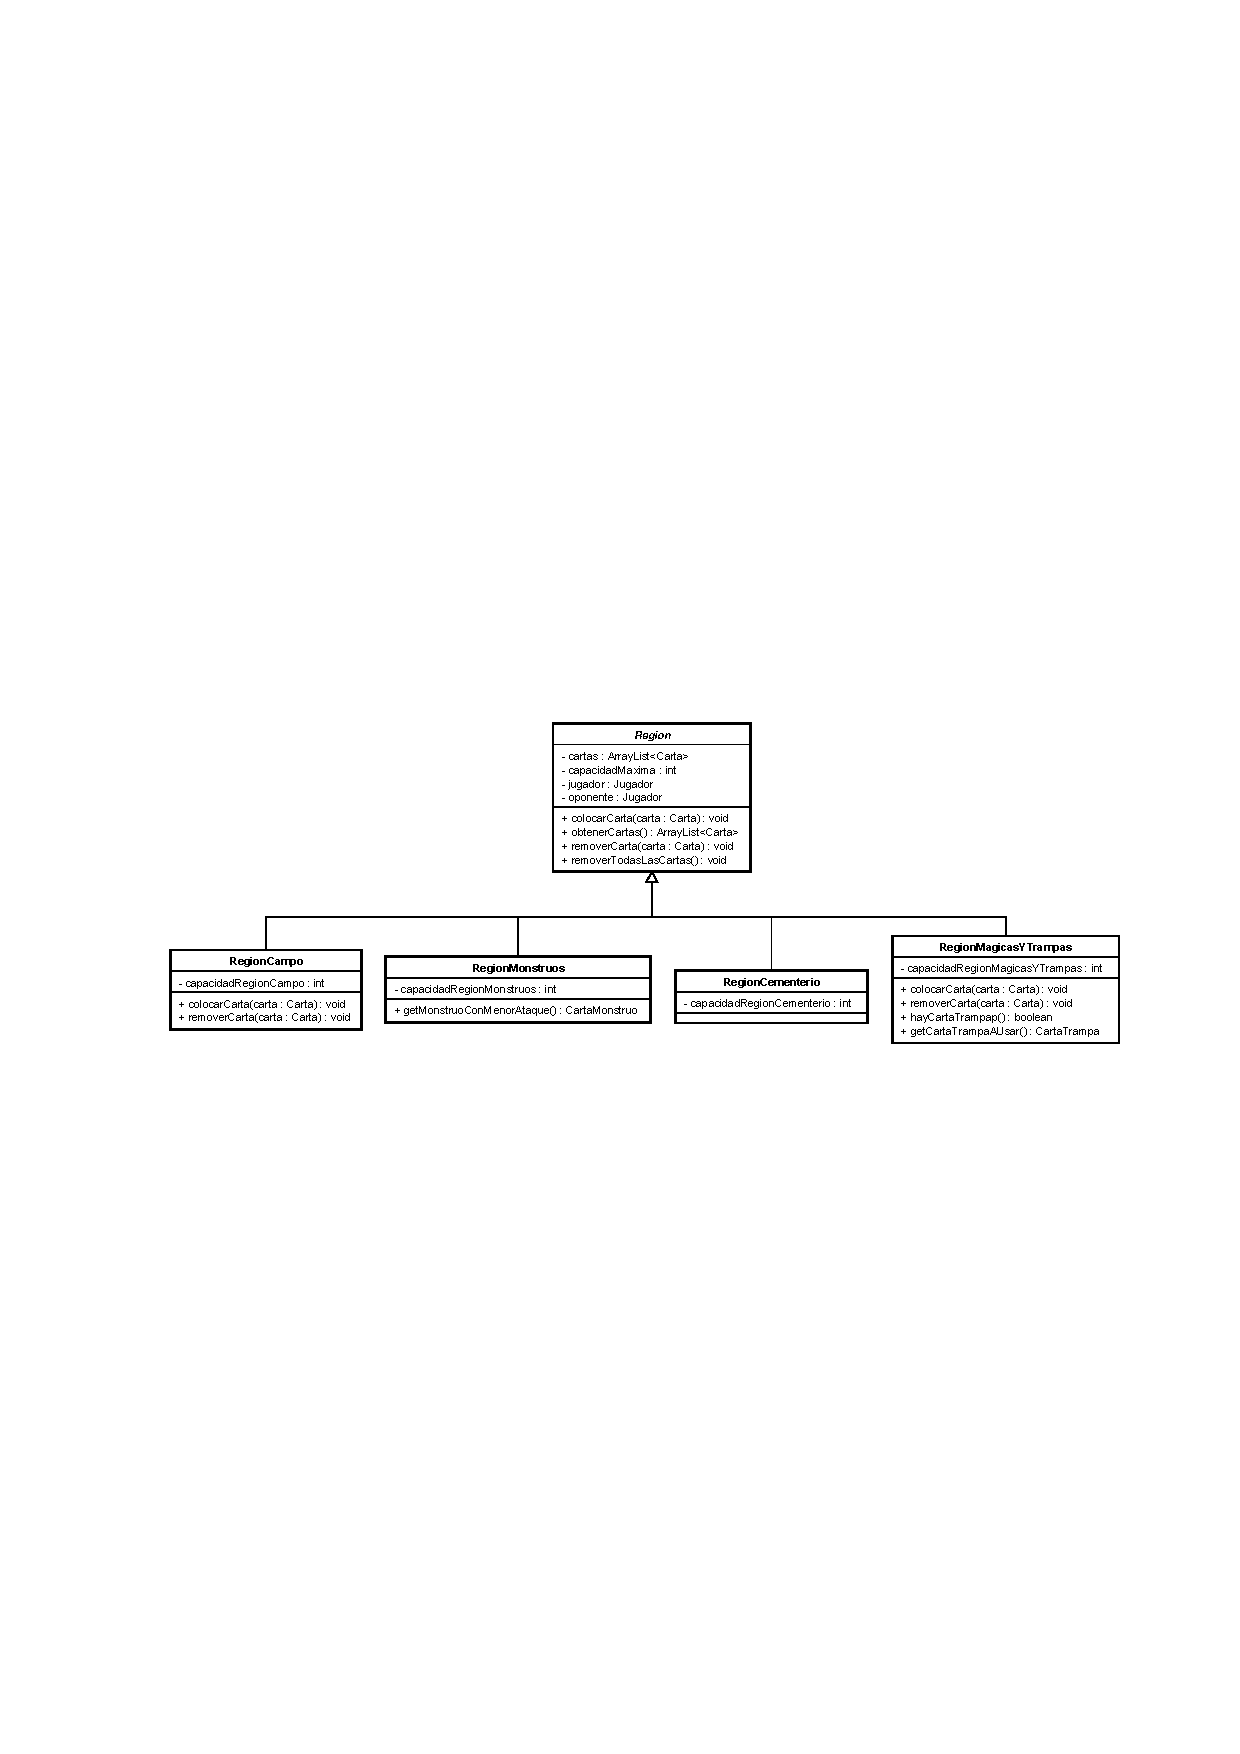
\includegraphics[scale=0.8]{includes/class_Regiones}
		\caption{Regiones.}
		\label{class_Regiones}
	\end{figure}
	
	\subsection{Vista}
	
	El diagrama (Figura \ref{class_Vista}) muestra las distintas variaciones que puede tener la \texttt{Escena} a través del juego (Se habla más sobre esto en la sección diagramas de secuencia, Figura \ref{estado_Estados_Vista}), acompañado de los métodos principales que contiene la interface \texttt{Escena} y algunos específicos de cada escena específica.
	
	\begin{figure}[H]
		\centering
		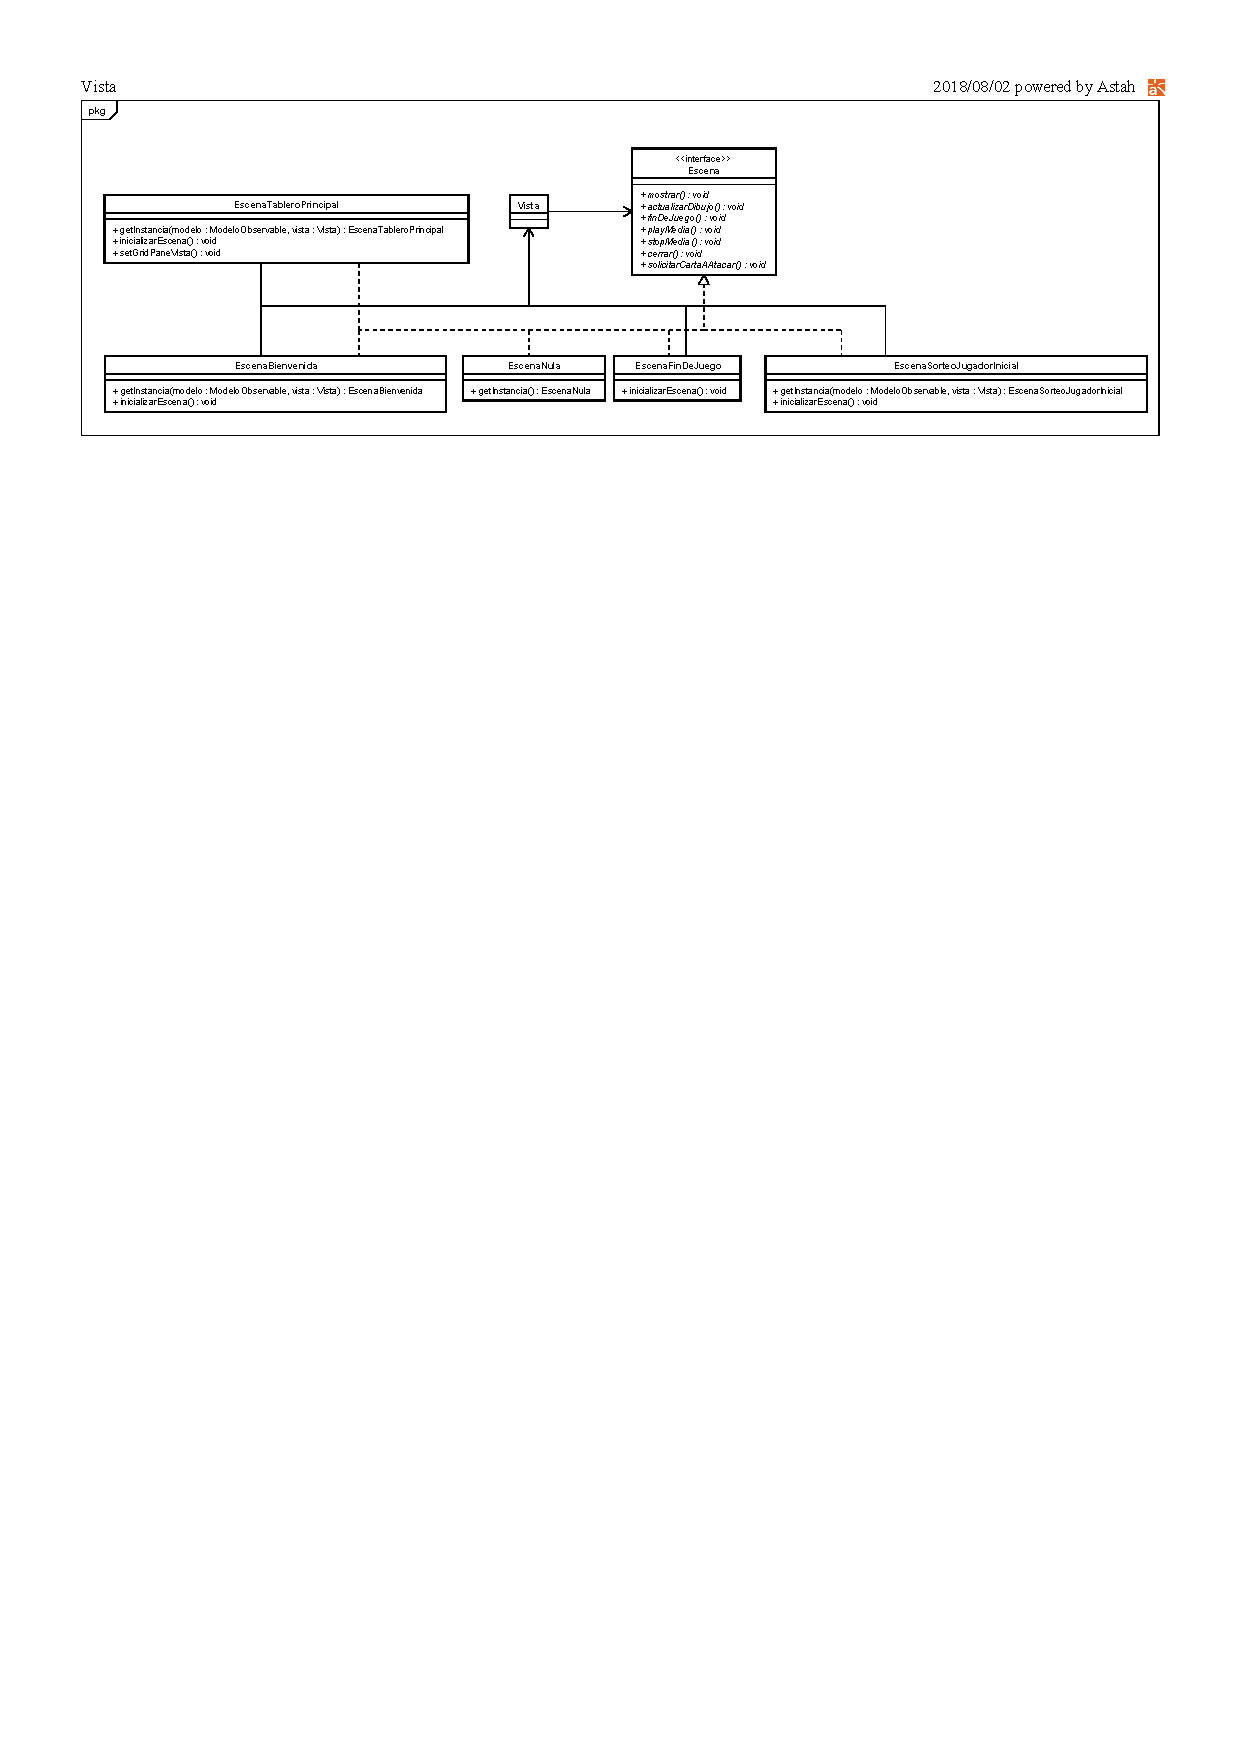
\includegraphics[scale=0.8]{includes/class_Vista}
		\caption{Vista.}
		\label{class_Vista}
	\end{figure}
	
	
	\clearpage
	\section{Diagramas de secuencia}
	
	A continuación mostraremos y explicaremos algunas de las secuencias mas complejas presentes en el programa.
	
	\subsection{Ataque de carta sin trampas, parte MVC}
	
	En este diagrama (Figura \ref{seq_Ataque_de_carta_sin_trampas}) veremos que ocurre, del lado de la \texttt{Vista}, \texttt{Modelo} y \texttt{Controlador} cuando un usuario ataca con una de sus \texttt{CartaMonstruo} a una \texttt{CartaMonstruo} de su oponente. Vamos a suponer para este diagrama que ya fue jugada alguna carta Monstruo (Por lo que le es posible al jugador atacar) y se cumplen las condiciones necesarias para que el jugador pueda realizar un ataque.
	
	La secuencia comienza con el jugador oprimiendo \quotes{atacar} en la carta Monstruo que se encuentra en su región durante la fase de ataque. Luego de que ocurre este evento, le llega al controlador un aviso de que el jugador quiere atacar, por lo que, luego de verificar que se cumplan todas las condiciones para que se efectúe un ataque (Si estas no se cumplen se le da un aviso al usuario), le pide al usuario que quiere atacar que elija su \quotes{Carta a atacar}. Esto se realiza en la vista, haciendo que le aparezcan al jugador las opciones para su ataque, que serían las cartas enemigas a las cuales el puede atacar (Vale notar aquí que, en caso de que no haya cartas para atacar, se efectúa el ataque directamente al jugador oponente).
	
	Una vez hecha la selección, se registra el ataque de la carta (Ya que una misma carta no puede atacar dos veces en el mismo turno) y se le delega al Modelo que efectúe el ataque. Antes de hacer esto, se ingresa a la \texttt{FaseTrampa}, en la cual se verifica si, durante este ataque, es necesario activar o no alguna \texttt{CartaTrampa}.
	
	\begin{figure}[H]
		\centering
		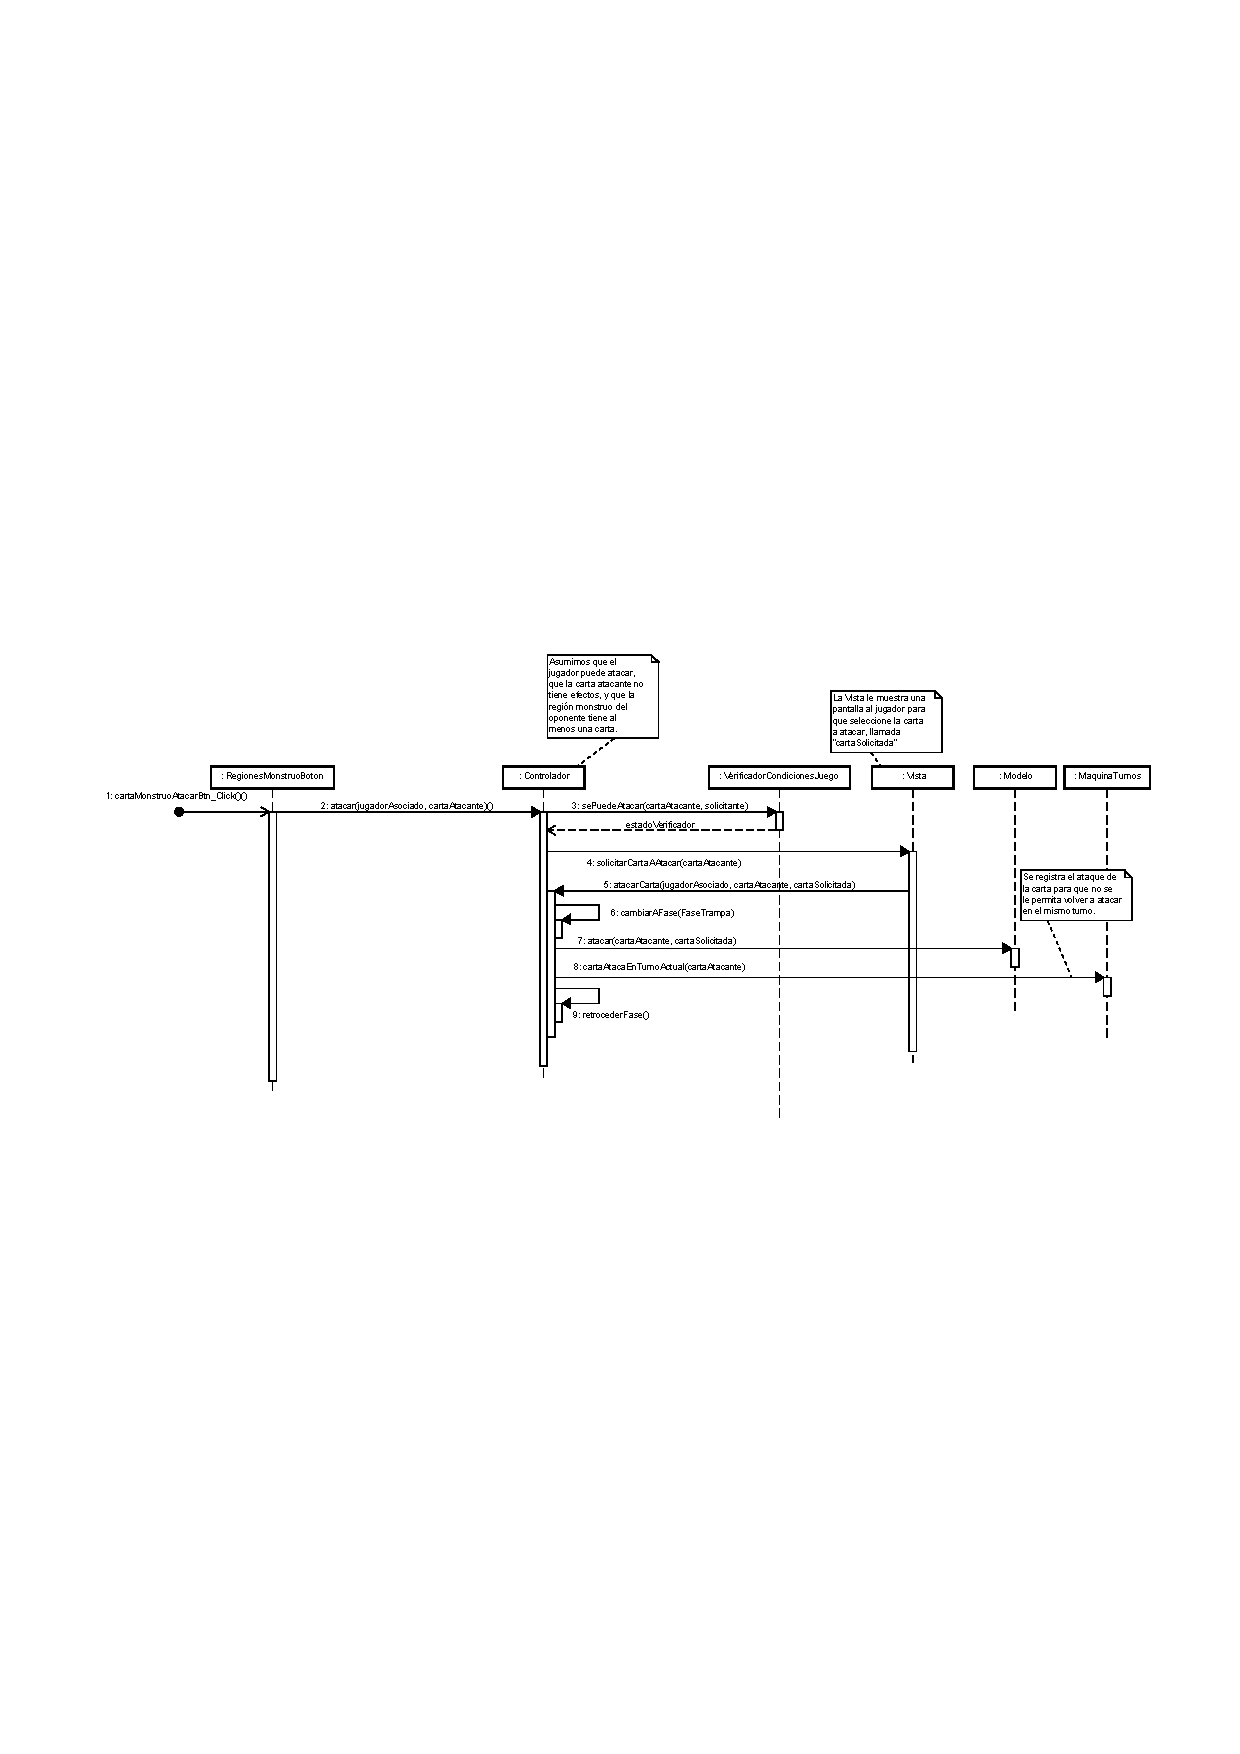
\includegraphics[scale=0.9]{includes/seq_Ataque_de_carta_sin_trampas}
		\caption{Diagrama de secuencia de un ataque de carta monstruo a otra sin cartas trampa en el campo.}
		\label{seq_Ataque_de_carta_sin_trampas}
	\end{figure}
	
	
	\subsection{Ataque de cartaMonstruo con mayor ataque a otra cartaMonstruo con menor}
	
	Este diagrama (Figura \ref{seq_Carta_con_mayor_ataque_ataca_a_carta_con_menor_ataque}) es una continuación del anterior (Figura \ref{seq_Ataque_de_carta_sin_trampas}) solo que concentrándose en que ocurre dentro del \texttt{Modelo} cuando se efectúa un ataque.
	
	Cuando le llega una solicitud de ataque al \texttt{Modelo}, este verifica que no haya cartas trampa en la región del oponente (Se realiza durante la \texttt{FaseTrampa} mencionada anteriormente), suponemos en este caso que no existen \texttt{CartaTrampa} en la región del oponente.
	
	De la manera que fue implementado, una \texttt{CartaMonstruo} ataca a otra \texttt{CartaMonstruo}, esta última, \quotes{recibe} el ataque de la otra. Cuando esto ocurre, la misma \texttt{CartaMonstruo} realiza el cálculo de puntos y decide cual es el resultado de la \quotes{pelea} entre ellas cartas. En nuestro caso, la carta \quotes{atacante} tiene mas puntos de ataque que la carta \quotes{atacada}, por lo que la atacada es destruida y enviada al cementerio para luego, disminuirle al jugador propietario de la carta que perdió la batalla los puntos de vida correspondientes.
	
	\begin{figure}[H]
		\centering
		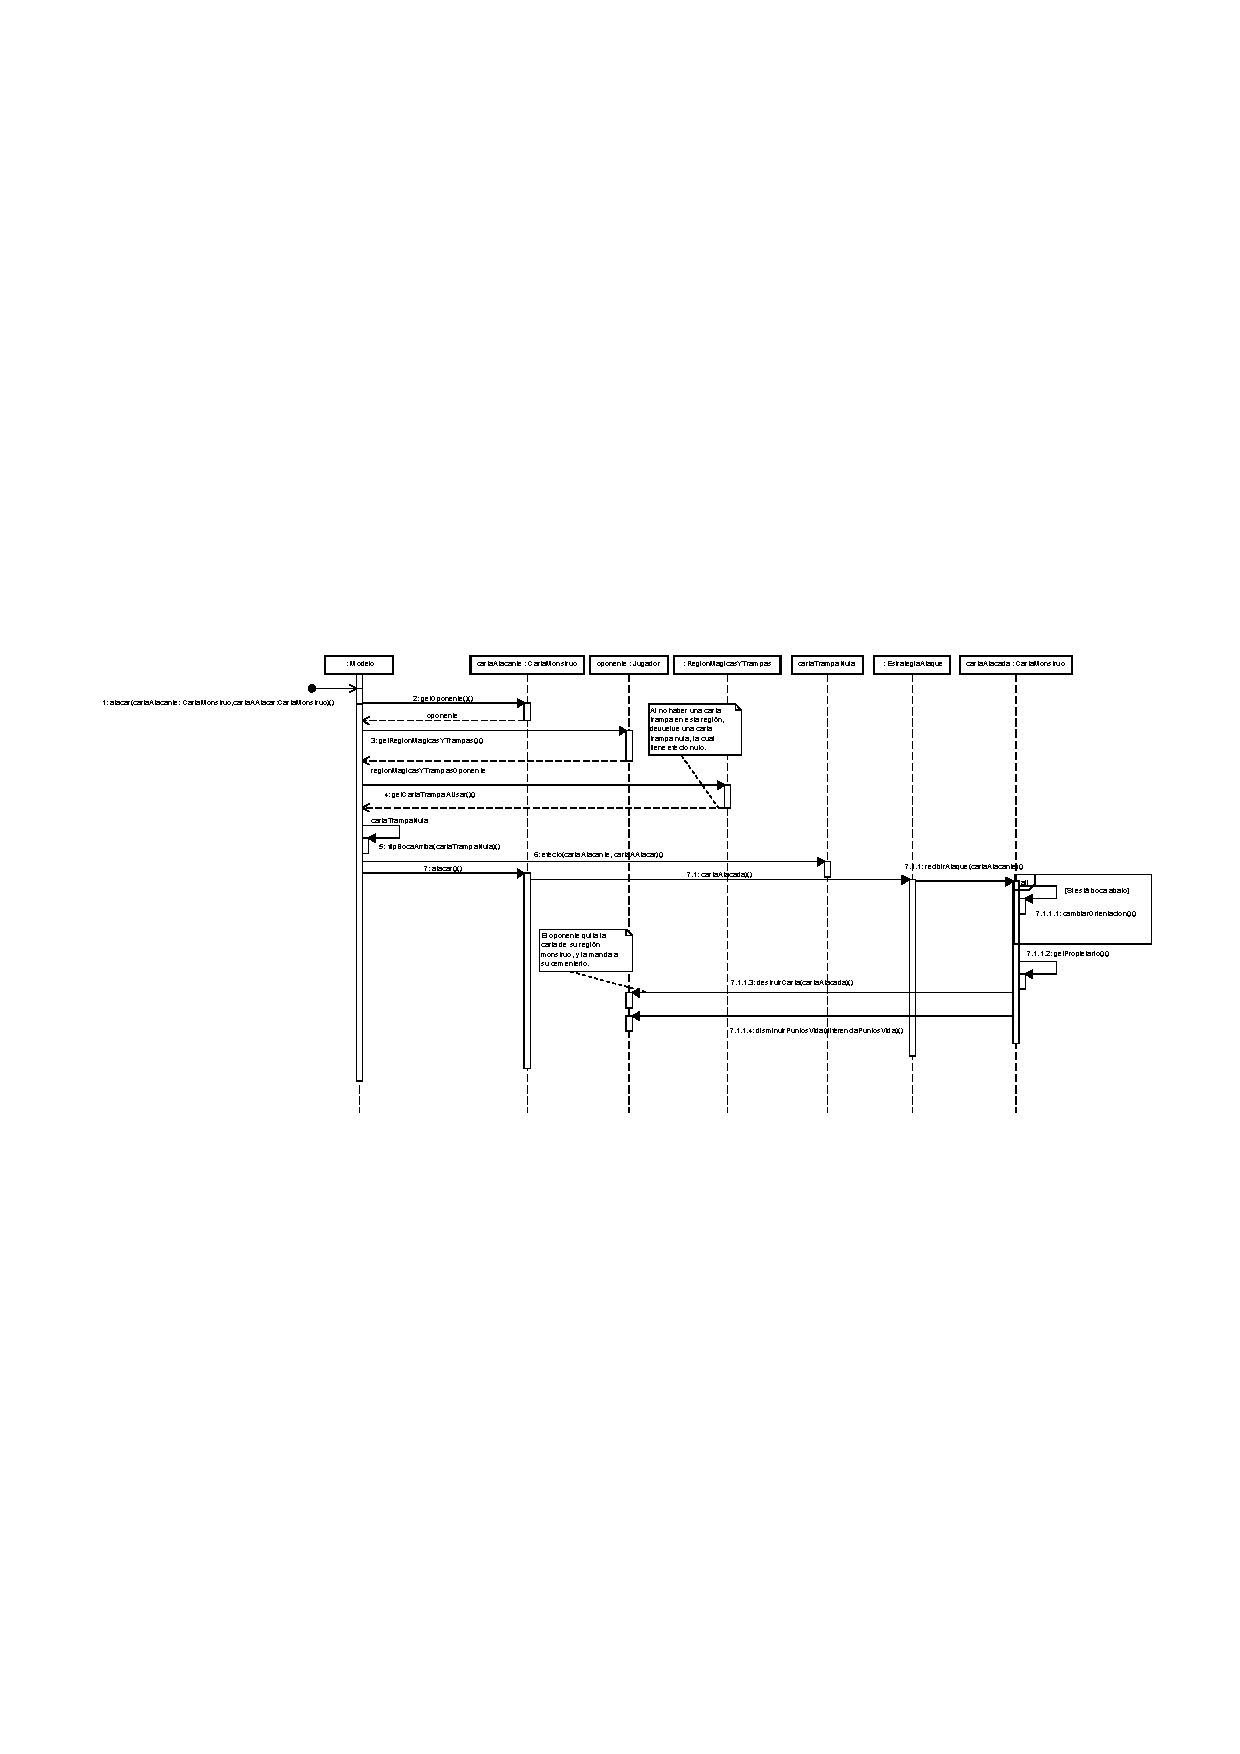
\includegraphics[scale=0.9]{includes/seq_Carta_con_mayor_ataque_ataca_a_carta_con_menor_ataque}
		\caption{Diagrama de secuencia de ataque de una carta monstruo a otra con menor ataque.}
		\label{seq_Carta_con_mayor_ataque_ataca_a_carta_con_menor_ataque}
	\end{figure}
	
	\subsection{Uso de carta Dark Hole desde la mano}
	
	En este diagrama (Figura \ref{seq_DarkHole_desde_la_mano}) veremos el caso en el que la carta \texttt{DarkHole} (que es del tipo \texttt{CartaMagica}) se juega desde la mano. Especificamos que se juega desde la mano ya que existe la posibilidad de que el usuario \quotes{posicione} la carta para ser usada cuando el lo desee.
	
	La secuencia comienza, al igual que con el caso de el ataque de la \texttt{CartaMonstruo}, desde la \texttt{Vista}. En este caso, el usuario presiona el botón correspondiente a \quotes{activar} la carta mientras esta se encuentra en su mano. Nuevamente, vamos a suponer que se cumplen todas las condiciones necesarias para que el jugador pueda activar esta carta (Que sea la fase correcta, que sea su turno, etc.). Cuando el botón se presiona, se realiza un pasaje de mensajes desde la \texttt{Vista} (que en este caso sería la \texttt{ManoVista}) por el \texttt{Controlador} hasta llegar al \texttt{Modelo}. Una vez en el modelo, se muestra la carta y se activa su efecto (Característica principal de las \texttt{CartaMagica} y \texttt{CartaTrampa}).
	
	Como la carta tiene como atributos al \texttt{Jugador} propietario de la carta y su \texttt{Oponente}, les envía el mensaje \quotes{destruirMonstruos} a ambos, haciendo que se destruyan y manden al \texttt{Cementerio} todos los monstruos que estaban colocados en cada \texttt{RegionMonstruos}. Por último, el modelo se encarga de quitar la carta \texttt{DarkHole} de la mano del \texttt{Jugador} que la usó y enviarla al \texttt{Cementerio}.
	
	\begin{figure}[H]
		\centering
		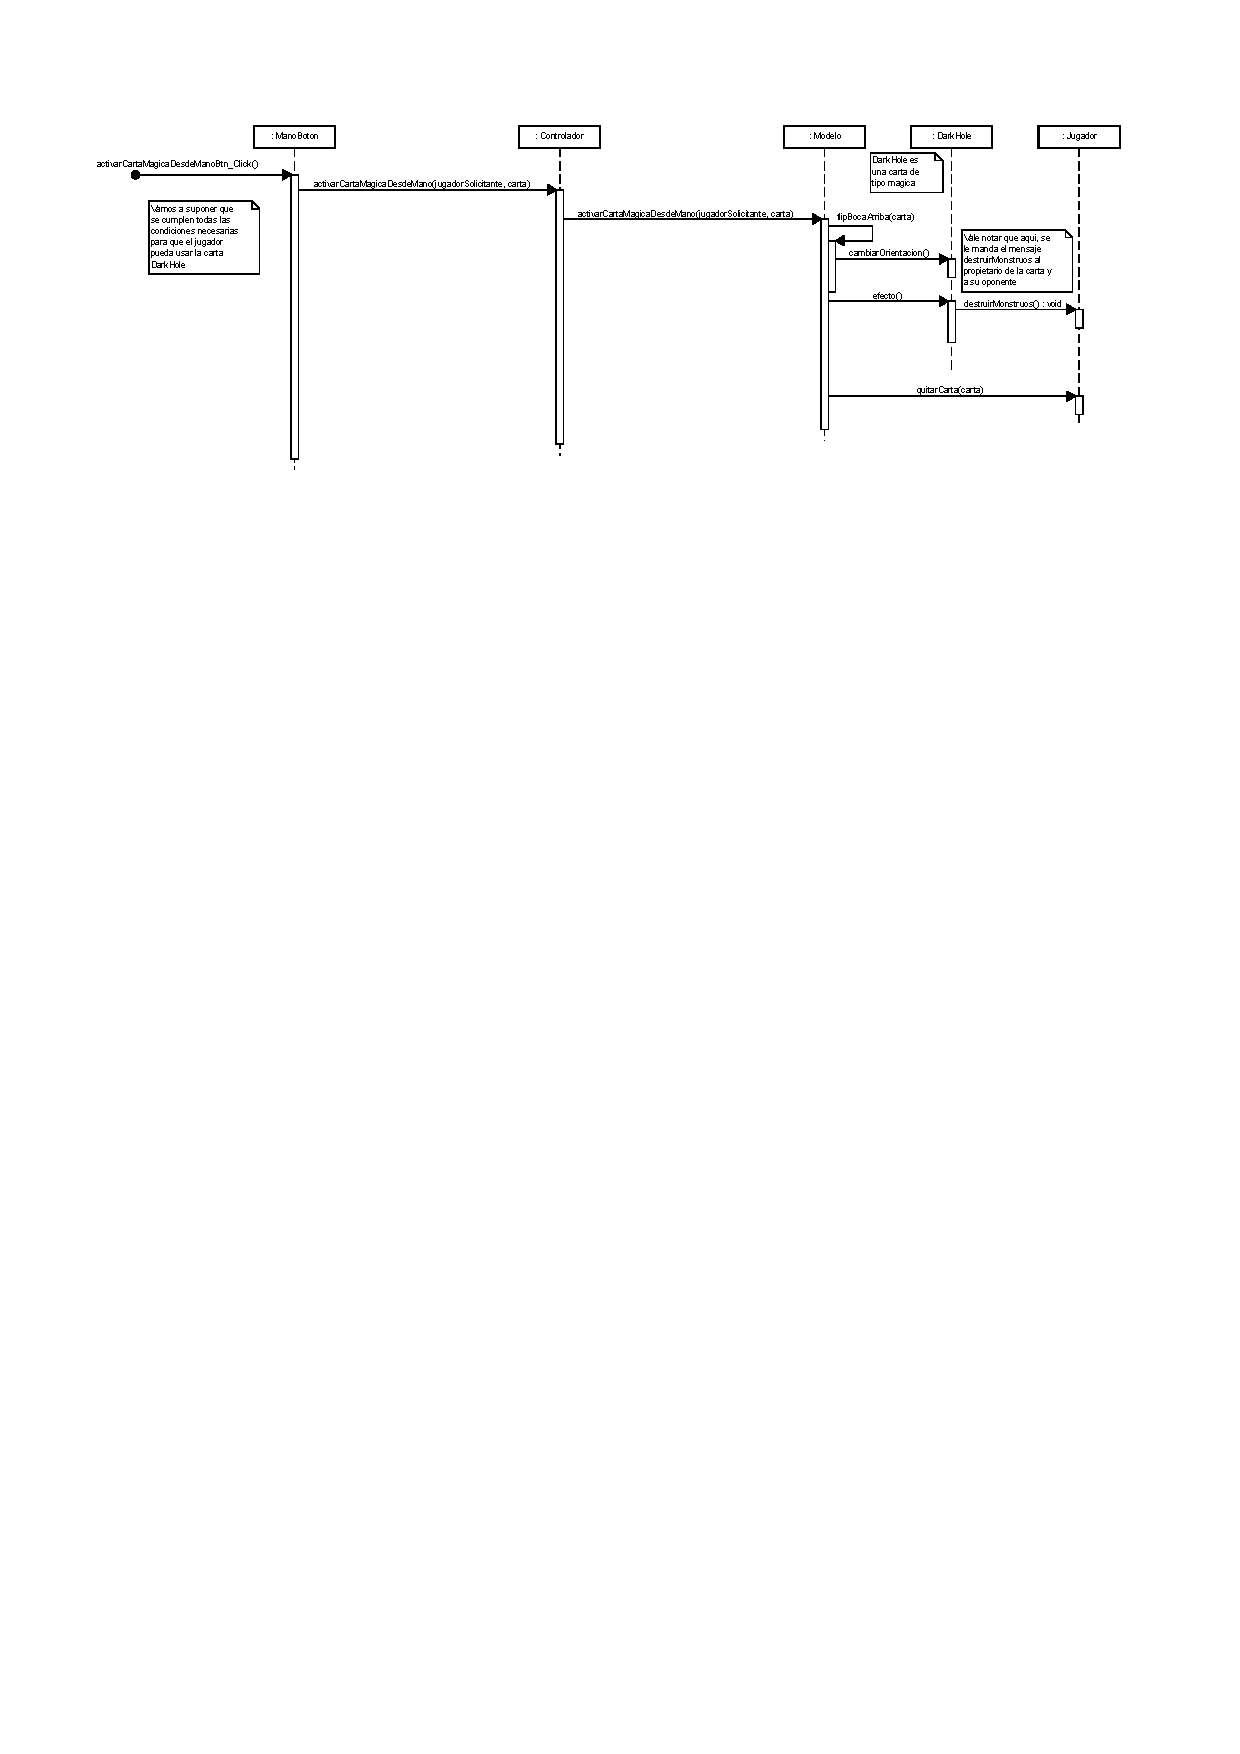
\includegraphics[scale=0.9]{includes/seq_DarkHole_desde_la_mano}
		\caption{Diagrama de secuencia de activación de carta mágica Dark Hole desde la mano del jugador.}
		\label{seq_DarkHole_desde_la_mano}
	\end{figure}
	
	\subsection{Uso de carta Monstruo come hombres}
	
	En este diagrama (Figura \ref{seq_Dragon_ataca_a_insecto_Come_Hombres_boca_abajo}) podemos ver el funcionamiento de la carta \texttt{ManEaterBug} o \quotes{Monstruo come hombres}.
	
	La secuencia en sí es muy parecida al caso visto en la figura \ref{seq_Carta_con_mayor_ataque_ataca_a_carta_con_menor_ataque} solo que, a la hora de \quotes{recibir} el ataque, nuestra \quotes{cartaAtacada} tiene un efecto. Este efecto se activa cuando el ataque es recibido y, en el caso de \texttt{ManEaterBug}, el efecto es que la \quotes{cartaAtacante} es destruida si ataca a este monstruo mientras se encuentra boca abajo.
	
	Lo importante a notar aquí es que, al igual que con las \texttt{CartaMagica} y \texttt{CartaTrampa}, hay algunas \texttt{CartaMonstruo} que tienen un efecto. Este efecto, al igual que con las cartas ya mencionadas, es propio de la misma y el \quotes{que hacer} del efecto esta inscripto en cada carta.
	
	\begin{figure}[H]
		\centering
		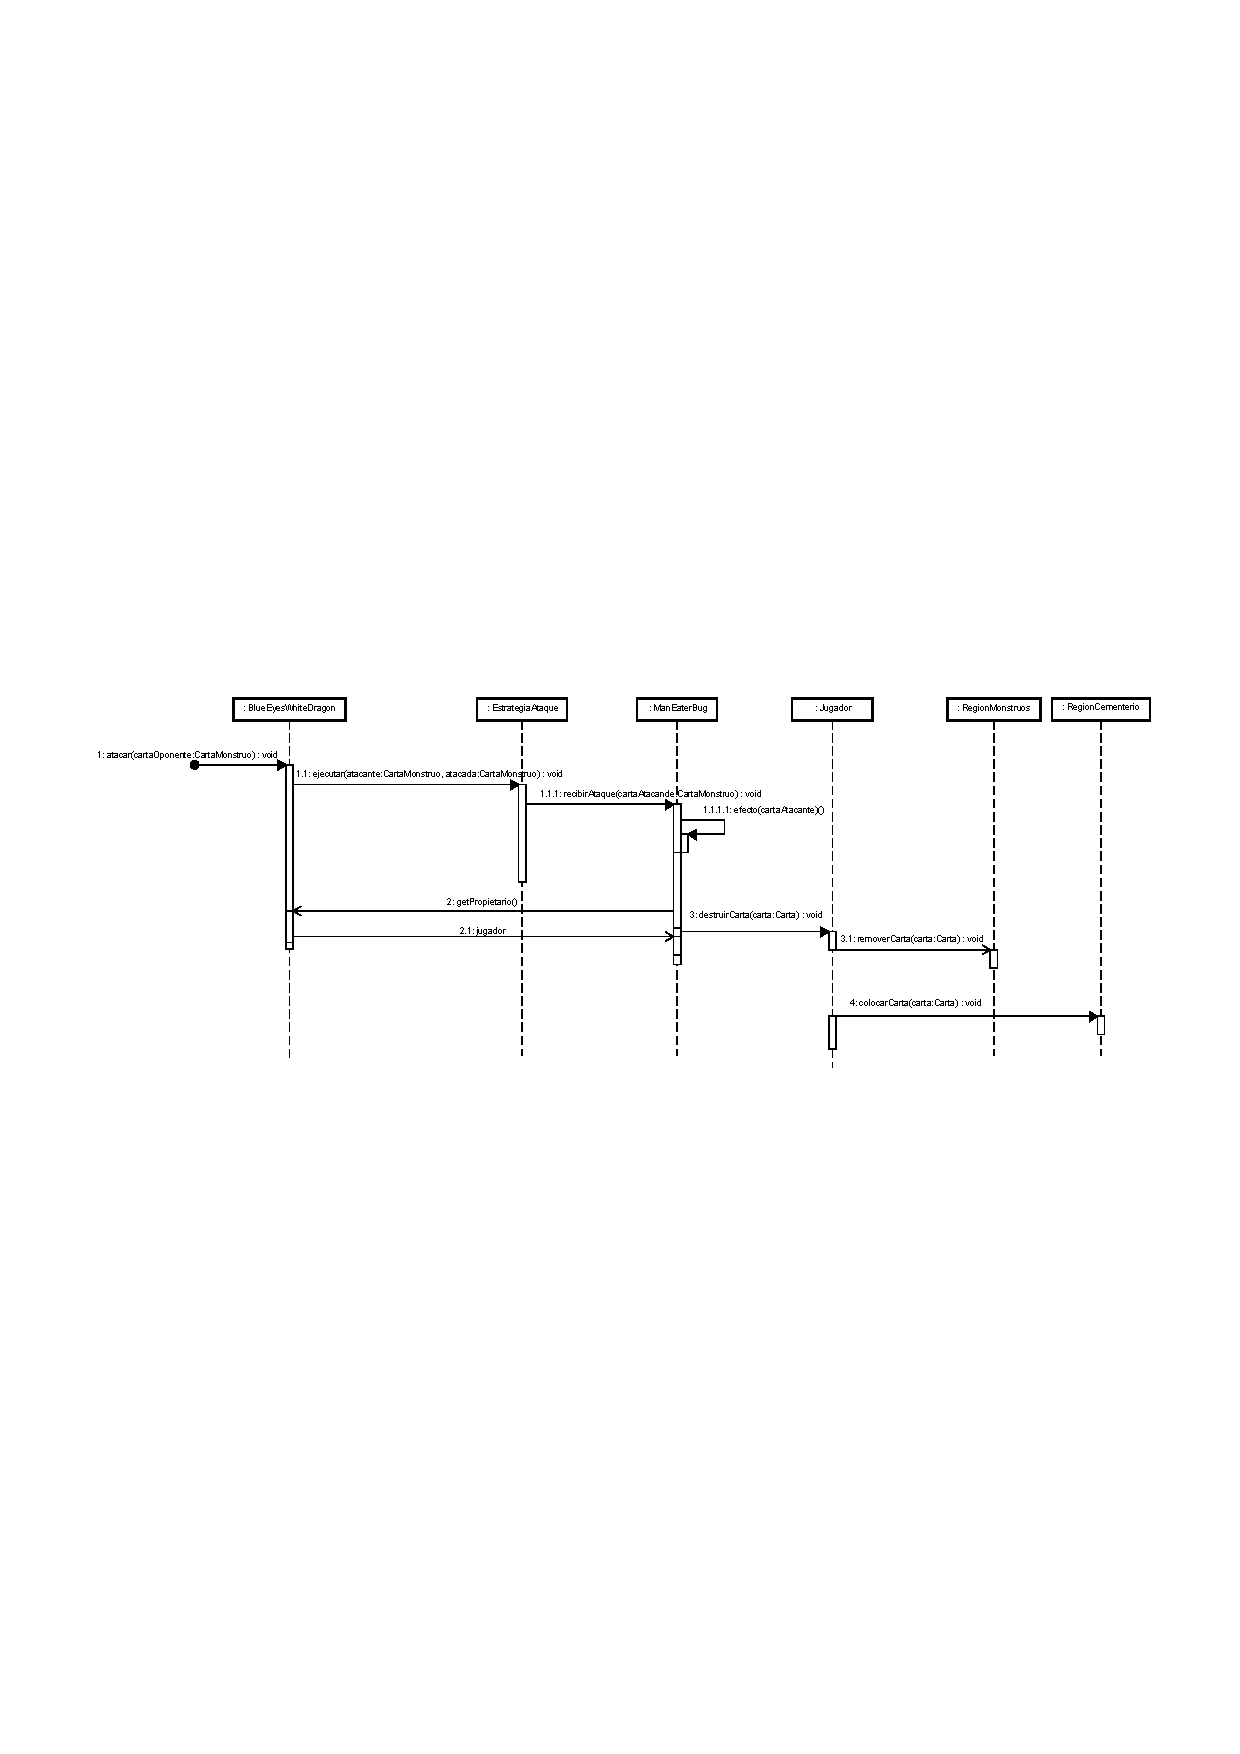
\includegraphics[scale=0.9]{includes/seq_Dragon_ataca_a_insecto_Come_Hombres_boca_abajo}
		\caption{Diagrama de secuencia de carta monstruo dragón atacando a la carta Come-Hombre que se encuentra boca abajo.}
		\label{seq_Dragon_ataca_a_insecto_Come_Hombres_boca_abajo}
	\end{figure}
	
	\subsection{Carta ingresando a region monstruos}
	
	En el diagrama (Figura \ref{seq_Ingresa_carta_a_region_monstruo_mostrando_interaccion_en_MVC}) veremos que ocurre cuando ingresa una \texttt{CartaMonstruo} a la \texttt{RegionMonstruo}, específicamente las notificaciones que se realizan con los observadores. Este diagrama esta basado en una \texttt{CartaMonstruo} ingresando a \texttt{RegionMonstruo}, pero la secuencia con las cartas \texttt{CartaMagica} y \texttt{CartaTrampa} es similar.
	
	La secuencia comienza cuando el \texttt{Jugador} ingresa una \texttt{CartaMonstruo} a la \texttt{Region}. Esta se agrega y luego, se notifica a los observadores de \texttt{RegionMonstruo} (En este caso el \texttt{Modelo}) que ingreso una carta, luego, el \texttt{Modelo} se encarga de ver de donde viene la notificación para después, notificarle específicamente a \texttt{RegionesMonstruoGrid} que ingresó una carta. Una vez recibido el mensaje, la parte de la \texttt{Escena} asociada a esta región se actualiza.
	
	Finalmente, se le notifica a la \texttt{RegionCampo} que ingreso una nueva carta monstruo, esta región luego le pide a la \texttt{RegionMonstruo} la \quotes{ultima carta en ingresar}. Una vez obtenida la carta, se le aplica el efecto de la \texttt{CartaCampo}.
	
	\begin{figure}[H]
		\centering
		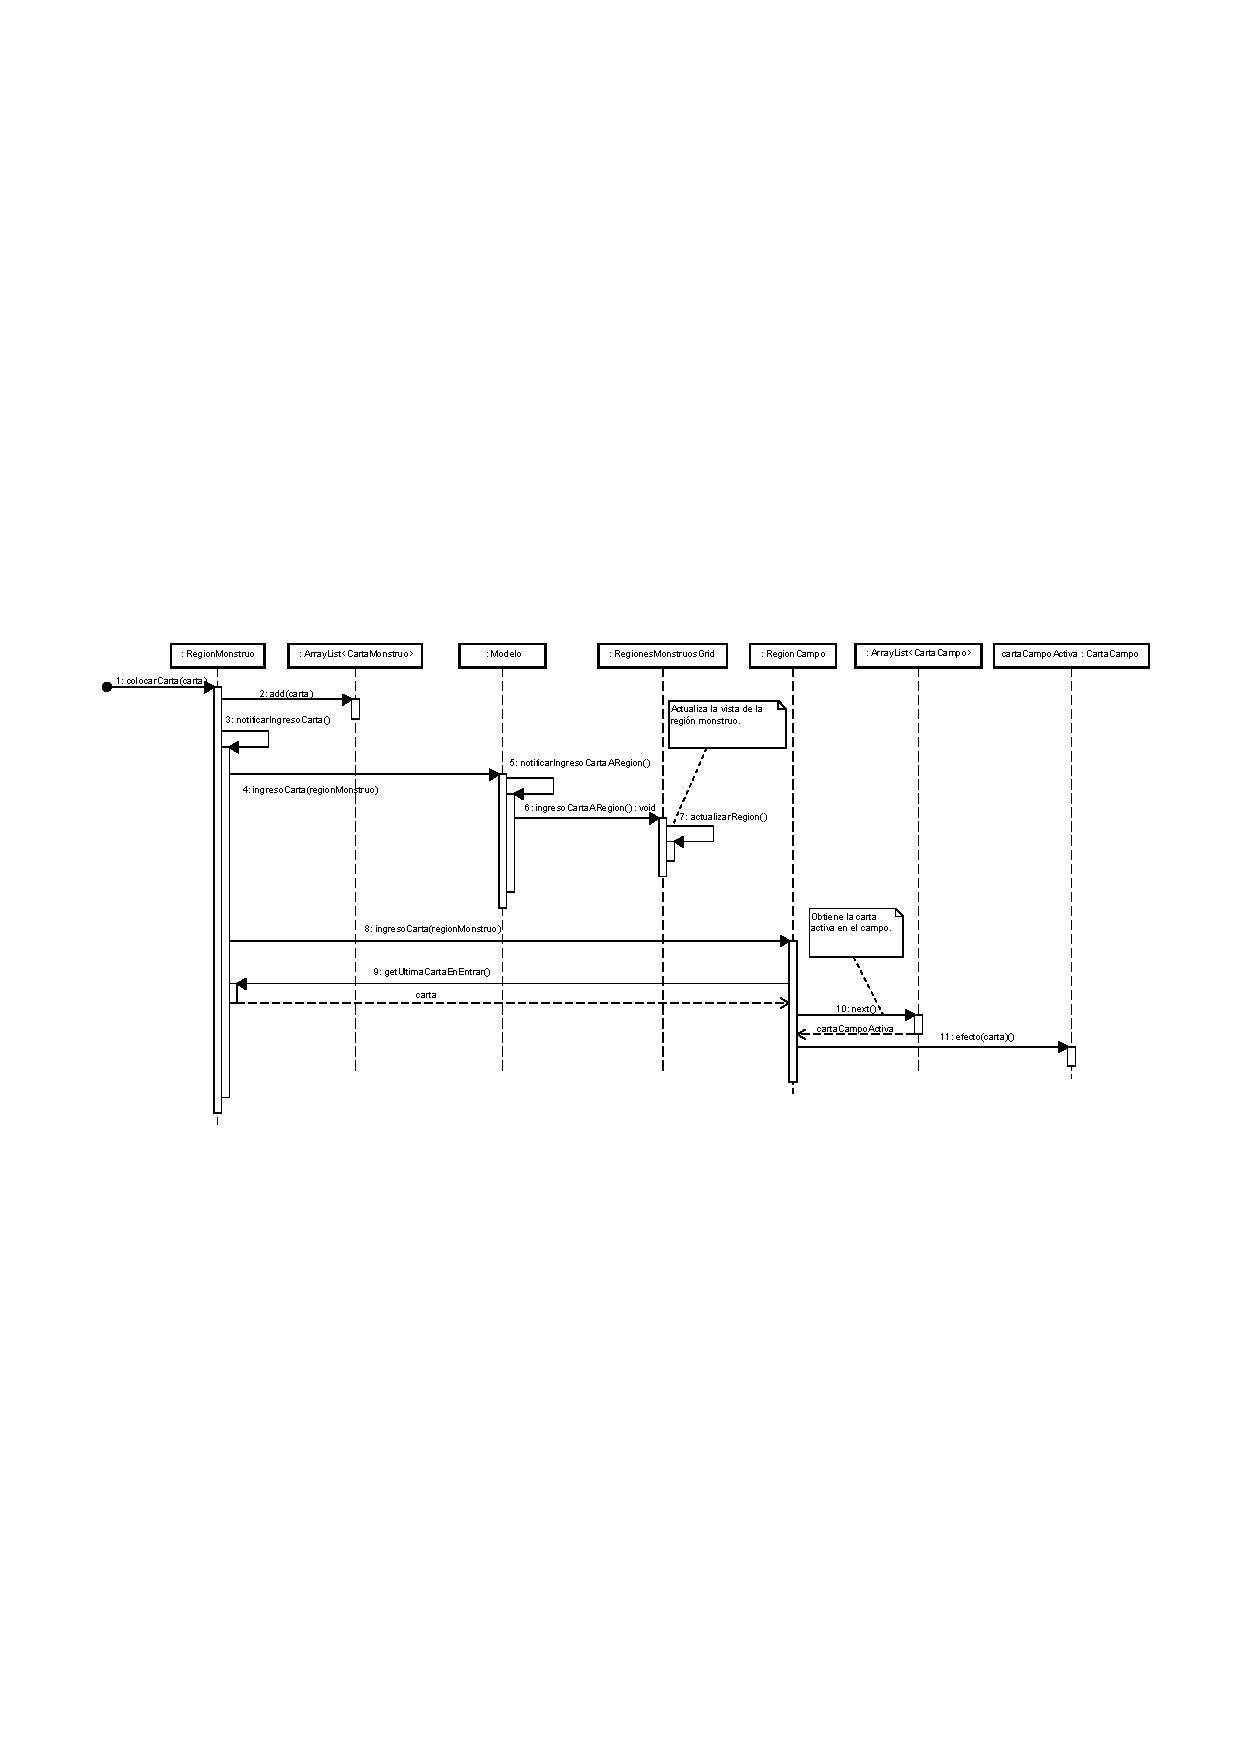
\includegraphics[scale=0.8]{includes/seq_Ingresa_carta_a_region_monstruo_mostrando_interaccion_en_MVC}
		\caption{Diagrama de secuencia de una carta ingresando a la región monstruo.}
		\label{seq_Ingresa_carta_a_region_monstruo_mostrando_interaccion_en_MVC}
	\end{figure}
	
	\subsection{Diagrama de activación de carta campo}
	
	Veremos como es el proceso en el cual se ingresa una \texttt{CartaCampo} al juego (Figura \ref{seq_Se_activa_una_carta_campo_y_entran_cartas_monstruo_a_la_region}).
	Cuando se pide activar una \texttt{CartaCampo}, se le solicita desde el \texttt{Modelo} la \texttt{RegionCampo} del \texttt{Jugador} que solicitó activar la carta. Si esta región se encuentra vacía, se ingresa la \texttt{CartaCampo} en la misma, si ya había una \texttt{CartaCampo}, esta es reemplazada por la nueva, deshaciendo los efectos que producía la anterior.
	
	Cuando ingresa la carta campo a la región, se le notifica a sus observadores que ocurrió este evento, por lo que de ahora en más, a cualquier \texttt{CartaMonstruo} que ingrese a \texttt{RegionMonstruos} se le aplicara el \quotes{efecto} de la \texttt{CartaCampo}. Además, cuando ingresa la carta campo, se obtienen todas las cartas monstruo en los campos del jugador y su oponente, y se le aplica el efecto de la carta campo.
	
	\begin{figure}[H]
		\centering
		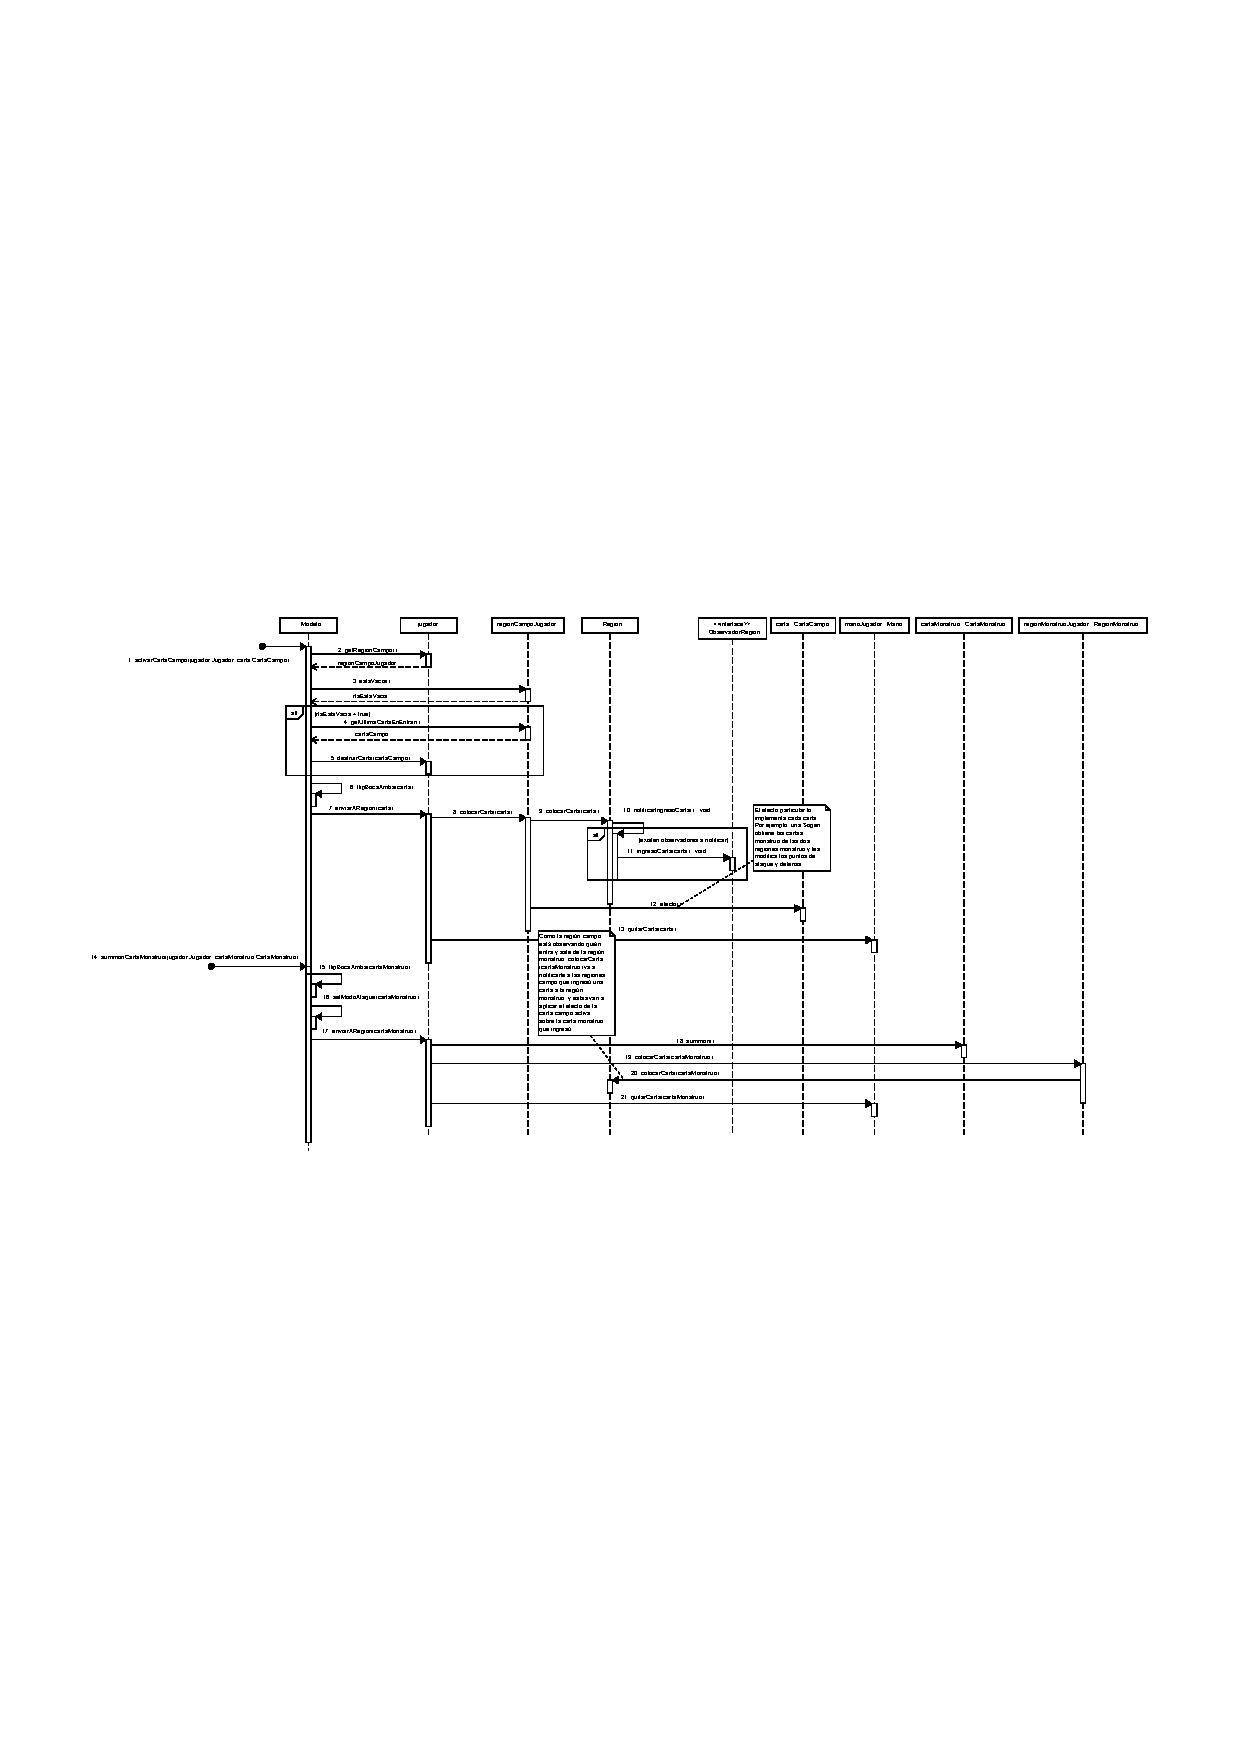
\includegraphics[scale=0.9]{includes/seq_Se_activa_una_carta_campo_y_entran_cartas_monstruo_a_la_region}
		\caption{Diagrama de secuencia de la activación de una carta campo y el posterior ingreso de una carta monstruo al campo.}
		\label{seq_Se_activa_una_carta_campo_y_entran_cartas_monstruo_a_la_region}
	\end{figure}
	
	\section{Diagramas de paquetes}
	
	En la figura \ref{paquetes} se muestra el diagrama de paquetes de la aplicación con sus dependencias internas más importantes. En general, los paquetes de excepciones suelen depender de todos los demás dentro de un paquete, ya que engloban todas las excepciones que se pueden lanzar para un dado paquete, por lo que no se especifica dicha dependencia con una flecha.
	
	Es importante notar que en el diagrama de paquetes puede verse cómo el patrón MVC define una arquitectura donde el modelo no tiene conocimiento del controlador ni de la vista, pero que el controlador y vista dependen mutuamente entre sí.
	
	\begin{figure}[H]
		\centering
		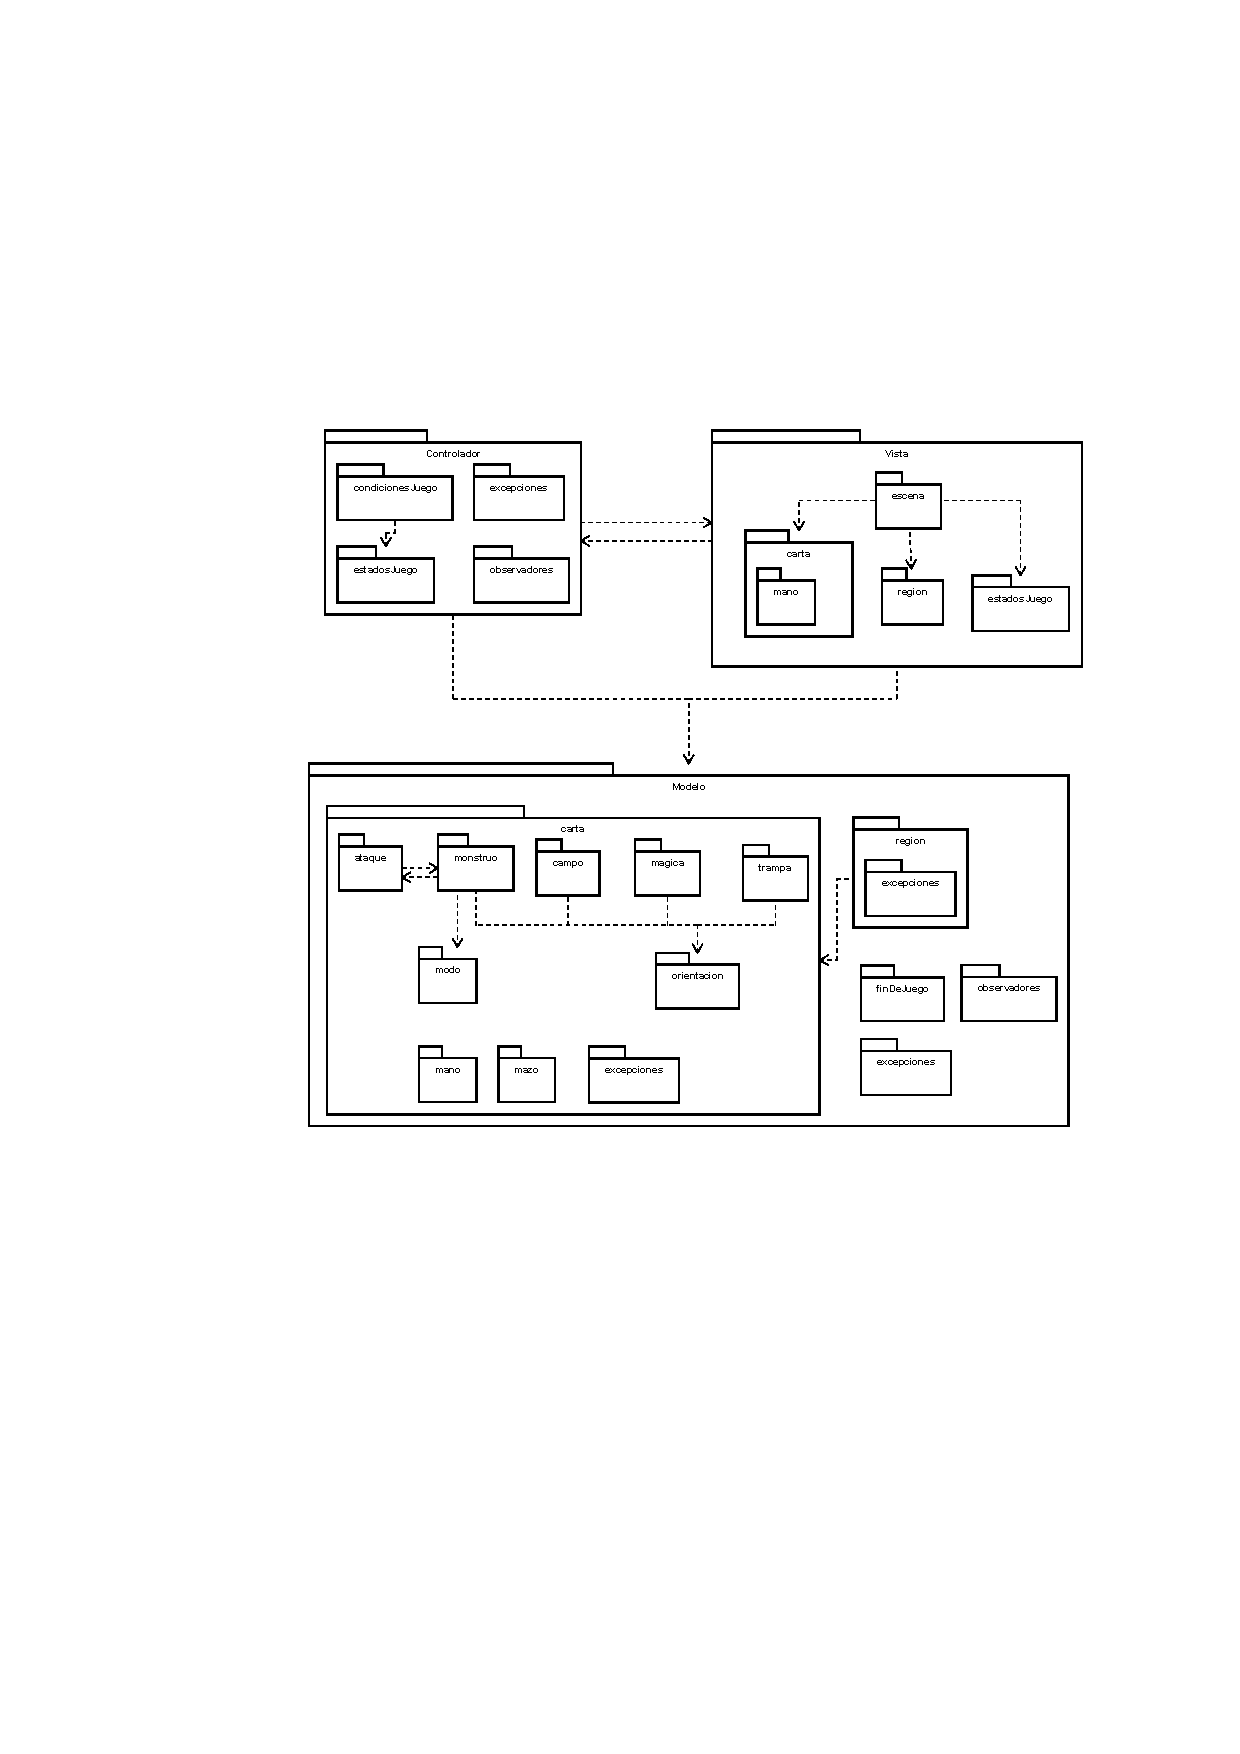
\includegraphics[scale=1]{includes/paquetes}
		\caption{Diagrama de paquetes y dependencias.}
		\label{paquetes}
	\end{figure}
	
	\section{Diagramas de estado}
	
	Aquí veremos como se manejan los estados de algunas de las componentes del juego. Indicando que ocurre en cada sección y como se realiza la transición a las próximas.
	
	\subsection{Diagrama de escena}
	
	Aquí (Figura \ref{estado_Estados_Vista}), podemos ver como va cambiando la \texttt{Escena} mientras avanza el juego. Comenzamos diciendo que cada \texttt{Escena} (Ya sea de bienvenida, sorteo, tablero, etc) tiene la posibilidad de salir si se quiere, pasando a \quotes{Vista confirmación cerrar programa} de una manera u otra.
	
	El juego comienza en la \quotes{Vista de bienvenida}, en donde los usuarios podrán ingresar sus nombres. Si se presiona \quotes{jugar} en esta escena, pasamos a la \quotes{Vista de sorteo} en la cual se elige que jugador va a comenzar su turno primero.
	
	Al finalizar esta etapa, pasamos a la \quotes{Vista tablero}. Esta vista es la principal del juego y es en donde se realizan todas las interacciones entre cartas, jugadores y demás. Cuando se dispara alguna de las \texttt{Causas Fin de Juego}, la escena pasa automáticamente a la \quotes{Vista fin de juego}, en donde se muestra al ganador del juego.
	
	\begin{figure}[H]
		\centering
		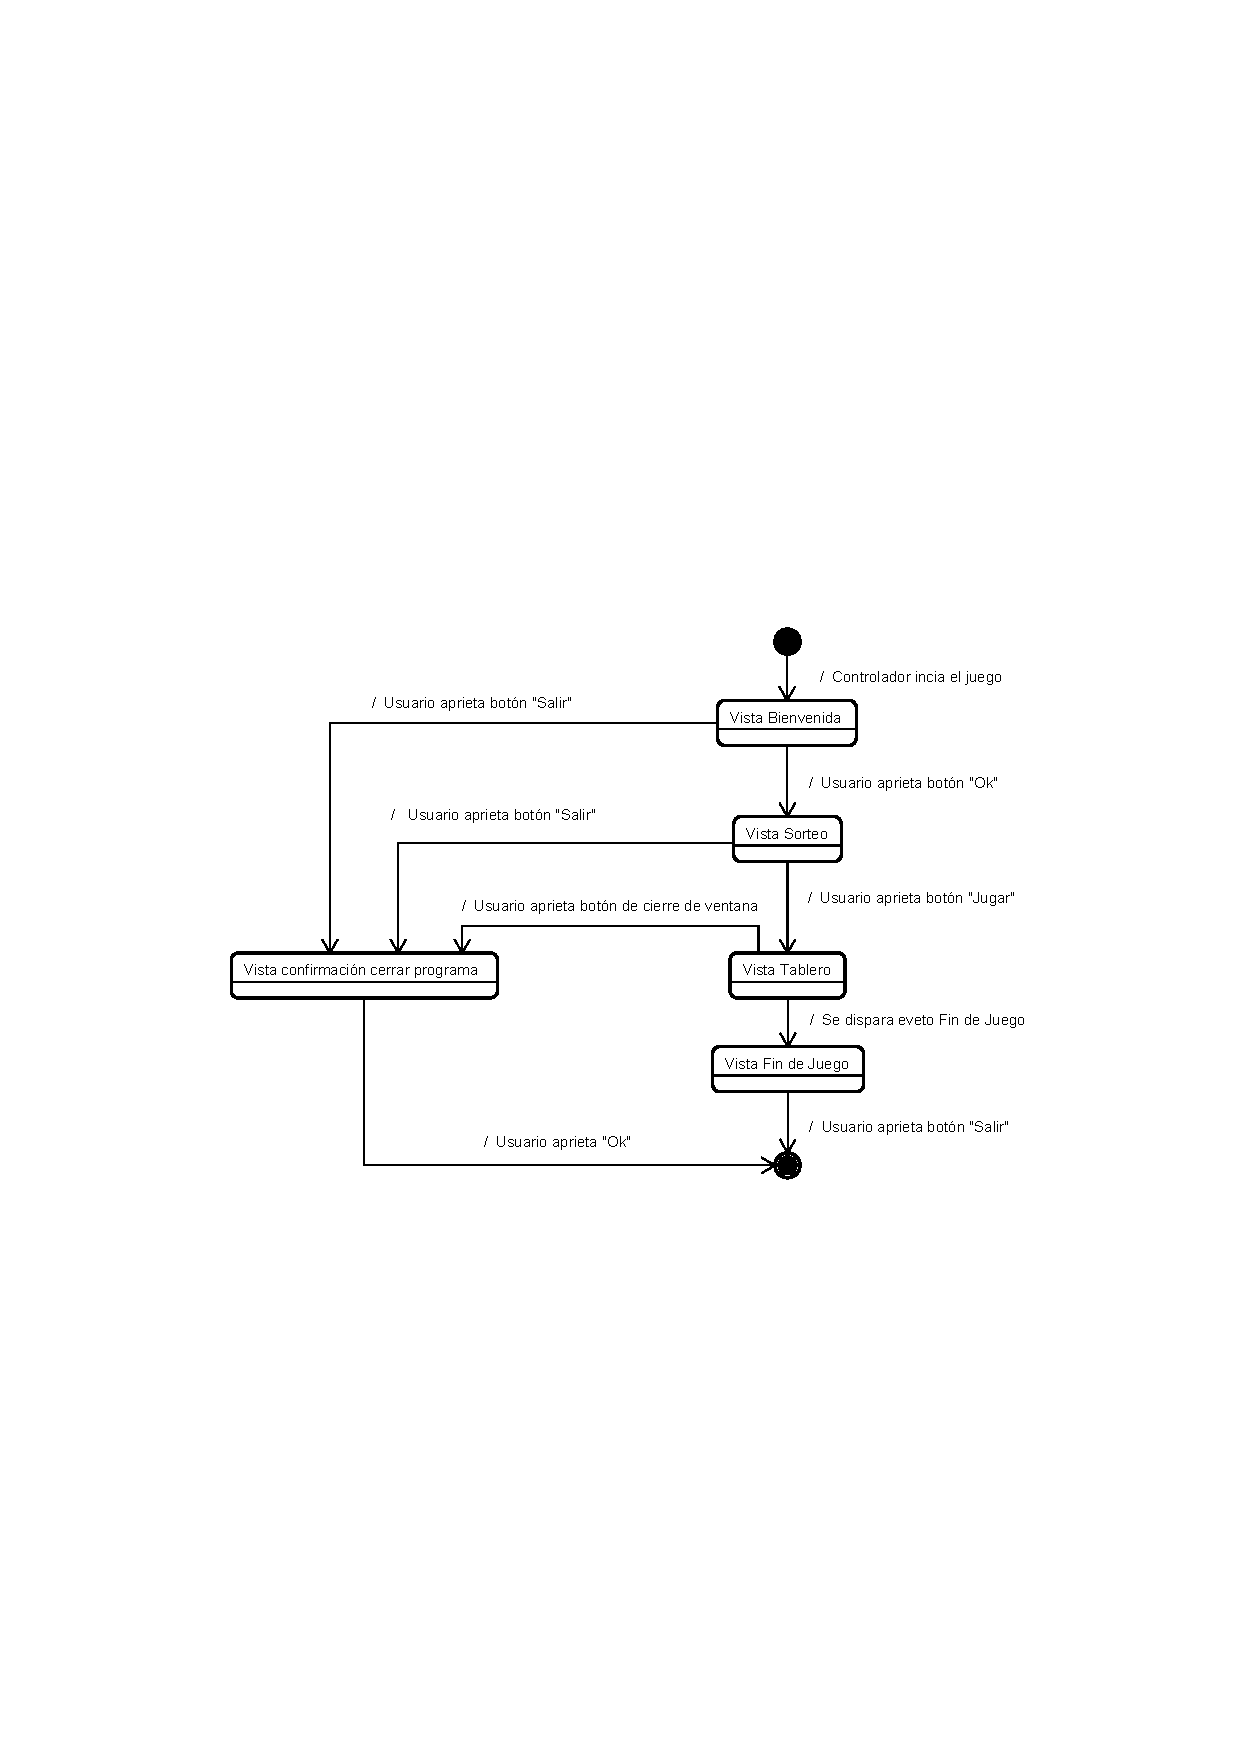
\includegraphics[scale=0.9]{includes/estado_Estados_Vista}
		\caption{Diagrama de estado de las diferentes escenas.}
		\label{estado_Estados_Vista}
	\end{figure}
	
	\subsection{Diagrama de fases}
	
	Vamos a analizar como se cicla entre las fases del juego (Figura \ref{estado_Maquina_de_Turnos}. Notamos que esto solo ocurre una vez ingresado a \quotes{Vista tablero}, previamente se eligió aleatoriamente que jugador comienza primero. También, se pueden \quotes{Saltear fases}, ya que es posible terminar el turno antes de llegar a la \texttt{FaseFinal}.
	
	Cada turno comienza con la \texttt{FaseInicial}, en la cual el \texttt{Jugador} toma automáticamente una carta. Luego de este evento, se pasa a la \texttt{FasePreparacion}. Aquí se pueden posicionar \texttt{CartaTrampa}, \texttt{CartaMagica} y \texttt{CartaCampo}, también \texttt{CartaMonstruo} pero solo una por turno. Luego de esta fase, si el jugador lo desea, puede pasar a la \texttt{FaseAtaque} en la cual, como su nombre lo indica, se le permite atacar (Como dijimos antes en el informe, no se puede atacar en el primer turno del juego). Lo interesante de esta fase es que está \quotes{anidada} con la \texttt{FaseTrampa} ya que, cada vez que se efectúa un ataque entre cartas, se pasa de la \texttt{FaseAtaque} a la \texttt{FaseTrampa} para verificar si es necesario activar algún efecto de alguna \texttt{CartaTrampa}.
	
	Por último, pasamos a la \texttt{FaseFinal}. Aquí se les permite a los jugadores activar sus \texttt{CartaMagica} y \texttt{CartaTrampa} que hayan sido posicionadas anteriormente. Cuando esta fase se termina, se pasa automáticamente al turno del próximo jugador y el ciclo comienza nuevamente.
	
	
	
	\begin{figure}[H]
		\centering
		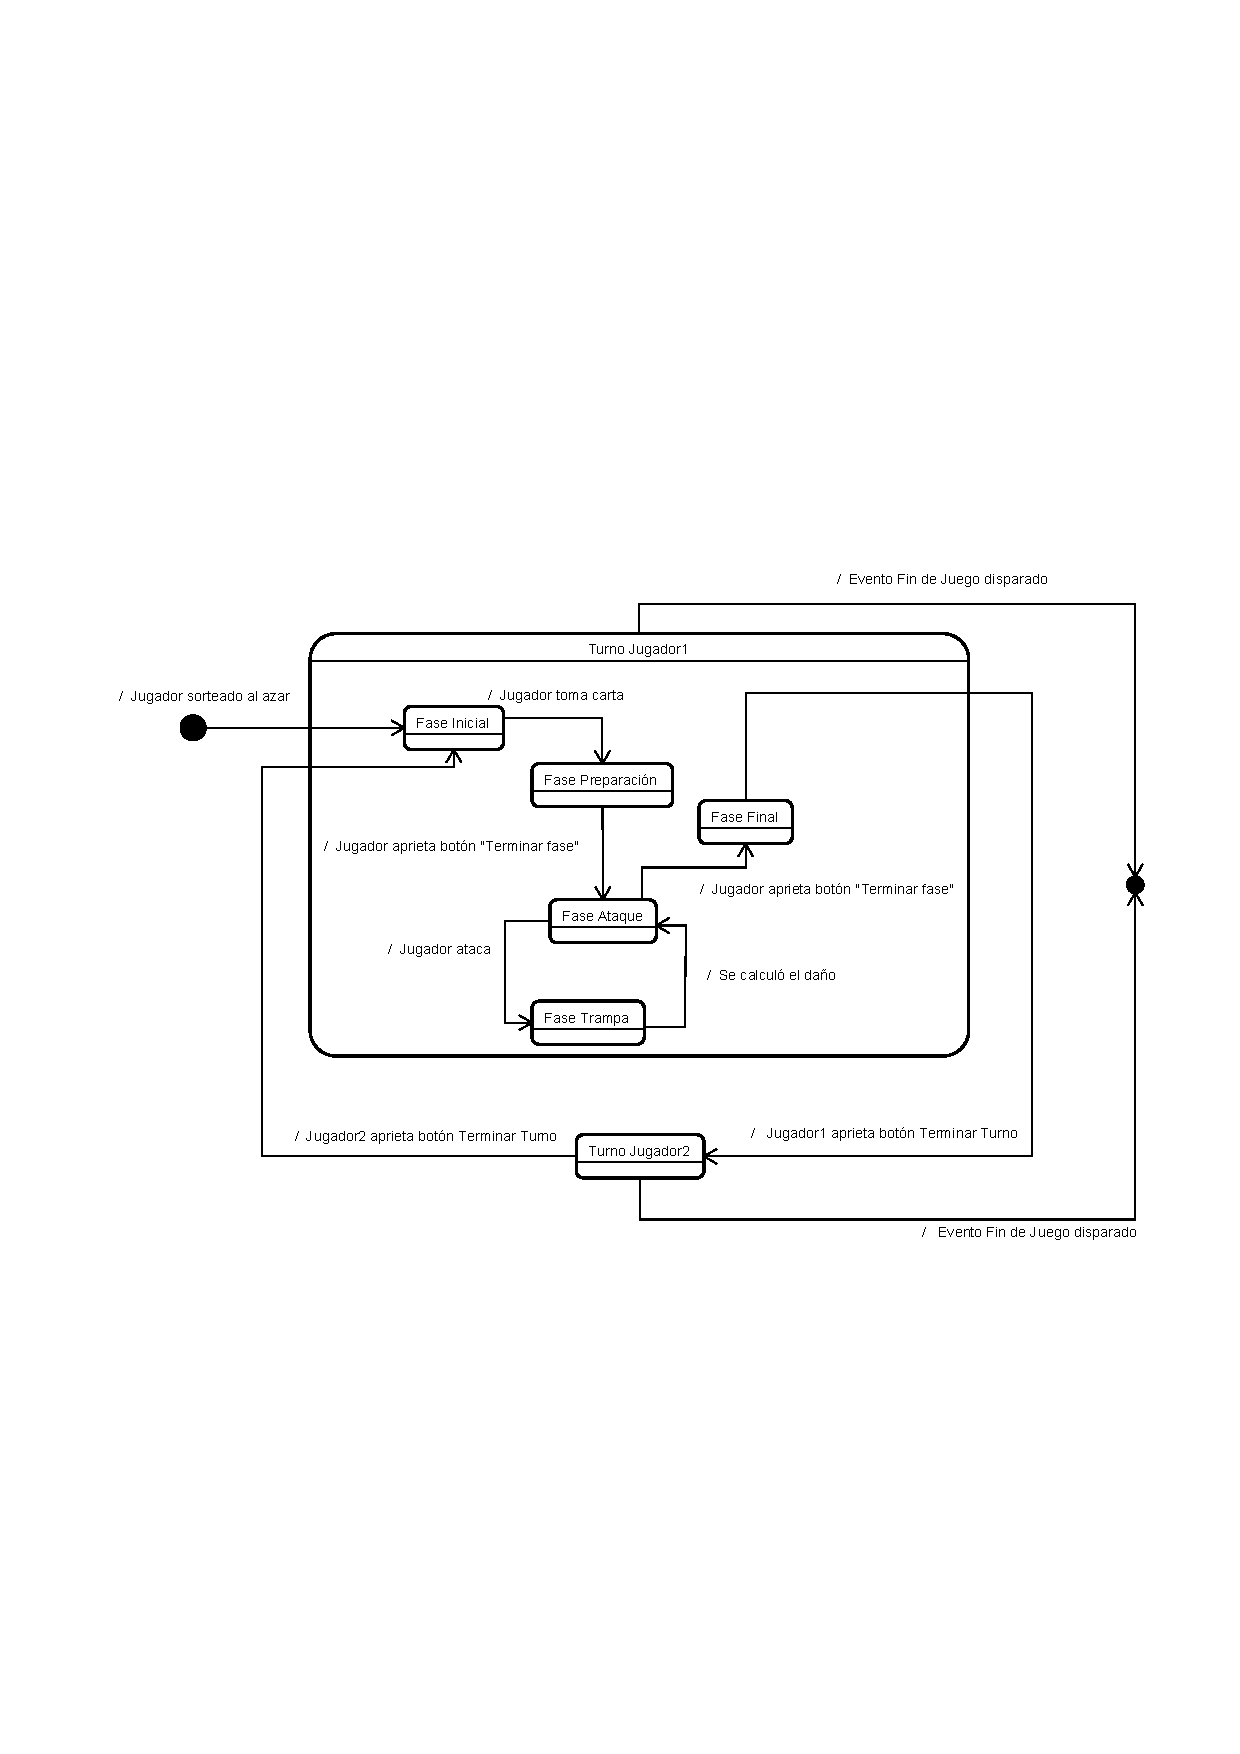
\includegraphics[scale=0.9]{includes/estado_Maquina_de_Turnos}
		\caption{Diagrama de estado de los turnos y fases.}
		\label{estado_Maquina_de_Turnos}
	\end{figure}
	
	\section{Detalles de implementación}
	
	Para el desarrollo del trabajo se utilizó la técnica de \textbf{Test Driven Development} para poder ir definiendo las entidades necesarias. Además, la organización del trabajo fue mediante \textbf{Pair Programming} para minimizar errores y tiempos de desarrollo, con reuniones tanto físicas y por videoconferencia.
	
	\subsection{Refactorizaciones}
	
	Para la realización de este trabajo práctico, se adoptó un desarrollo iterativo de mejoras ya que el código fue cambiando en reiteradas ocasiones debido a la implementación de múltiples refactorizaciones. 
	
	En un principio, se decidió que lo ideal era no utilizar una clase \texttt{Tablero} para modelar el juego y se logró la interacción entre los dos jugadores mediante la clase \texttt{Jugador}. A pesar de esto, a medida que se avanzó en la primera entrega, se tuvieron complicaciones de pasaje de mensajes y se optó por utilizar la clase \texttt{Tablero}. Luego de discutir con nuestro tutor sobre el diseño, se decidió que la utilización de un tablero como entidad arbitraria no era buena idea y que cada objeto del juego debiera comunicarse con otro para representar en mayor proporción la realidad, y no crear un árbitro/tablero que no existiese. Esto rompería con el \textbf{Principio SOLID de Responsabilidad Única} (el tablero estaría encargado de todas las acciones) y además, con el \textbf{Principio de Inversión de la Dependencia}, ya que todos dependerían de esta entidad.
	
	Entonces, se retomó la idea de que los dos jugadores se relacionen e interactuen entre ellos directamente y no mediante el árbitro/tablero. Se refactorizó para lograr eliminar el tablero, y se decidió que el ataque lo haga el jugador utilizando la carta y no que sea la carta la que atacaba al oponente. Esto también lo hablamos con el profesor y tomamos la decisión de que cada carta sea la que realiza el ataque y además, los efectos también sean implementados por cada carta. La implementación del efecto, en principio, la realizamos con una interfaz que obligaba a que todos tengan un efecto pero, como cada efecto era muy particular (recibía parámetros distintos) optamos por hacer que cada clase que use efecto tenga su método diferente al resto.
	
	Durante el desarrollo de la segunda entrega, se vio la necesidad de refactorizar nuevamente y convertir a cada tipo de carta en una clase abstracta, para que los monstruos específicos hereden de ellas y estos sean los que tengan las particularidades de cada una. Dicha decisión cumple con el \textbf{Principio de Sustitución de Liskov}, donde todas las clases hijas (Monstruos) son cartas monstruo y las cartas monstruo, son cartas. Esto aplica para toda la relación de cartas, y cumple el principio ya que todas las clases hijas se pueden ubicar en lugar de la clase padre. 
	
	También se refactorizó el cálculo de daño y ya no son las cartas monstruos las que restaban puntos al jugador, sino que el jugador se quita sus propios puntos de vida, cumpliendo así con el \textbf{principio SOLID abierto/cerrado}, ya que la clase debe estar cerrada al exterior para su modificación, pero abierta para su extensión.
	
	Durante la preparación de la entrega final se volvió a aplicar una refactorización que consistía en que el jugador (que hasta entonces, era el encargado de atacar y de llevar a cabo las tareas) ya no sería el encargado de implementar las estrategias de las cartas, sino que ahora ellas mismas son las que atacan y activan sus efectos. Esta refactorización, también cumple con el \textbf{Principio de Responsabilidad Única}, debido a que el jugador le hace pedidos a las cartas pero no le interesa como las cumplen.
	
	Una vez finalizado el modelo, se comenzó a implementar la interfaz gráfica y la idea con la que se comenzó fue conectarla directamente con el modelo pero nos dimos cuenta de que el usuario iba a interactuar con mas de lo que debía. Esta idea rompía con el \textbf{Principio de Segregación de la Interfaz} ya que el cliente solo debiera conocer lo que él solamente necesita, y luego de reunirnos con nuestro tutor, se decidió utilizar el patron de arquitectura MVC para separar correctamente las responsabilidades, minimizar dependencias, y aprovecha la segregación de interfaces.	
	
	
	\section{Excepciones}
	
	En esta sección hablaremos de las diferentes excepciones que fueron usadas en el programa, listándolas y explicando cuando ocurren cada una de ellas ya que varías son utilizadas para diferentes casos a través del programa. Cada uno de estos errores se manifiesta con una \quotes{alerta} en la vista, avisándole al usuario que ocurrió. De la manera que se manejó, dependiendo el caso en donde apareció la excepción, la alerta mostrada es diferente. Por ejemplo, lo que ocurre con \texttt{NoSePuedeAtacarError} a continuación.
	
	\subsection{Controlador}
	
	\begin{itemize}
		\item NoSePuedeAtacarError
		
		Este error ocurre cuando el jugador intenta atacar cuando no debe. Existen dos casos en donde este error puede aparecer, el primero es cuando se intenta atacar en una fase que no es la \texttt{FaseAtaque} y el otro, cuando se intenta atacar con una \texttt{CartaMonstruo} que ya atacó en el turno. Estos casos se diferencian con la alerta enviada. Si se dio el primer caso de la excepción, se muestra una alerta, si se dio el segundo, otra diferente.
		
		\item NoSePuedeCambiarOrientacionError
		
		El error ocurre principalmente cuando se intenta cambiar la orientación de una carta que ya fue cambiada de orientación en el mismo turno, acción que es invalida con respectos a los supuestos presentados anteriormente.
		
		\item NoSePuedeEnviarARegionCampoError
		
		Ocurre cuando se intenta jugar una \texttt{CartaCampo} en una fase que no es la \texttt{FasePreparacion}. 
		
		\item NoSePuedeEnviarCartaMonstruoARegionError
		
		Ocurre cuando se intenta jugar una \texttt{CartaMonstruo} en una fase que no es la \texttt{FasePreparacion}.
		
		\item NoSePuedeEnviarMyTARegionError
		
		Ocurre cuando se intenta jugar una \texttt{CartaTrampa} o una \texttt{CartaMagica} en una fase que no es la \texttt{FasePreparacion}.
		
		\item NoSePuedeUsarMyTError
		
		Este error se da cuando se intenta usar una \texttt{CartaMagica} o \texttt{CartaTrampa} que fue posicionada en una fase que no es la \texttt{FaseFinal}
		
		\item SeTerminaronLasFases
		
		El error se da cuando se llega a la \texttt{FaseFinal} y el \texttt{Jugador} presiona \quotes{Avanzar fase}, en este caso no se le notifica el error al usuario con una alerta, sino que pasa automáticamente al turno del próximo \texttt{Jugador}.
		
	\end{itemize}
	
	\subsection{Modelo}
	
	\begin{itemize}
		\item SacrificiosInsuficientesError
		
		Como su nombre lo indica, este error se da cuando el \texttt{Jugador} intenta \quotes{invocar} una \texttt{CartaMonstruo} que requiere \texttt{Sacrificio} pero no hay suficientes cartas en la \texttt{RegionMonstruos} para sacrificar.
		
	\end{itemize}
	
	\section{Conclusiones}
	
	Se desarrolló una aplicación que implementa de manera simplificada el juego de cartas Yu-Gi-Oh! utlizando el lenguaje de programación Java y la plataforma JavaFX para la interfaz gráfica.
	
	Se estudiaron diferentes patrones de diseño que resultaron de utilidad para modelar varias partes del programa, y en particular, el patrón Observer ya que permitió desarrollar adecuadamente los diferentes eventos que había que procesar y también minimizar acoplamientos entre clases.
	
	Por otro lado, el uso del patrón de arquitectura MVC nos permitió desarrollar independientemente el controlador y la vista a pesar de que se realizaban en paralelo varias refactorizaciones del modelo.
	
	Por último se logró aprender cómo la programación orientada a objetos permite identificar entidades independientes minimizando el acople entre ellas y facilitando el desarrollo de aplicaciones de complejidad media a elevada.
	
	%-------------------------------%
	%								%
	%			Seccion				%
	%								%
	%-------------------------------%
	\appendix
	\section{Referencias}
	% Removes 'Referencias' title from 'thebibliography'.
	\begingroup
	\renewcommand{\section}[2]{}
	\begin{thebibliography}{10}
		\bibitem{libro_fontela1} Fontela, Carlos - \emph{Programación Orientada a Objetos con Smalltalk, Java y UML.} - 3\textsuperscript{ra} edición - Versión Beta 0.6.
		
		\bibitem{fowler_model} Fowler, M. - \hyperref{https://martinfowler.com/distributedComputing/purpose.pdf}{}{}{What's a model for?}
		
		\bibitem{reglas_juego} \hyperref{https://www.yugioh-card.com/en/rulebook/SD_RuleBook_EN_10.pdf}{}{}{Yu-Gi-Oh! TRADING CARD GAME rulebook}
	\end{thebibliography}
	\endgroup
	
\end{document}
